\documentclass[journal]{IEEEtran}

\usepackage[T1]{fontenc}
\usepackage[utf8]{inputenc}
\usepackage[french]{babel}
\usepackage{amsmath,amssymb,amsthm}
\usepackage{graphicx}
\usepackage{array}
\usepackage{algorithm}
\usepackage{algorithmic}
\usepackage{microtype}
\usepackage{booktabs}
\usepackage{tikz}
\usetikzlibrary{arrows.meta,positioning,shapes,calc}
\usepackage{pgfplots}
\pgfplotsset{compat=1.17}

\newtheorem{proposition}{Proposition}

\graphicspath{{figures/}}
\begin{document}

\title{MCAD : Un masque contextuel pour relier les requêtes OLAP aux objectifs stratégiques de l'organisation}

\author{Habib~Benaouda, Sidi~Mohamed~Benslimane, Zohra~Slama%
\thanks{Les auteurs sont affiliés au Département d'informatique de l'Université Djillali Liabès, Sidi Bel Abbès, Algérie. Les coordonnées peuvent être adaptées aux exigences du lieu de publication visé.}%
}

\maketitle

\begin{abstract}
Les entrepôts de données et les systèmes OLAP demeurent des infrastructures centrales pour le pilotage stratégique ; pourtant, la plupart des plateformes analytiques exécutent encore les requêtes sans expliciter leur contribution réelle aux objectifs métier. Les approches existantes de personnalisation et de recommandation OLAP se concentrent principalement sur les profils utilisateurs et l'historique de navigation, tandis que les approches sensibles au contexte et fondées sur les graphes de connaissances ne modélisent que partiellement l'environnement décisionnel. Aucune de ces lignes de recherche ne fournit un mécanisme formel permettant de mesurer, requête par requête et session par session, dans quelle mesure une requête OLAP contribue effectivement à un objectif stratégique donné.

Cet article introduit le \emph{Masque Contextuel de l'Analyse Décisionnelle} (MCAD). MCAD modélise le contexte de l'analyse décisionnelle sous la forme d'un graphe de connaissances contextuel (CKG) reliant dimensions, mesures, KPI, contraintes, scénarios, unités et fenêtres temporelles. Il représente un objectif stratégique global comme un ensemble de contraintes analytiques ancrées dans le CKG au moyen de nœuds virtuels décrivant les cellules analytiques minimales requises pour leur évaluation. Chaque requête analytique est compilée en un plan de requête canonique, vérifiée par un prédicat explicable de validité contextuelle, puis évaluée au regard de l'ensemble des contraintes de l'objectif rendues calculables grâce à cette requête. MCAD établit ainsi un pont explicite entre les objectifs analytiques (requêtes OLAP) et les objectifs métier, en filtrant les requêtes non contributives et en fournissant des indicateurs de progression vers l'objectif visé. Les résultats empiriques rapportés ici doivent être lus comme des \emph{preuves au niveau prototype} : sur les charges évaluées, MCAD préserve la couverture analytique utile tout en supprimant les exécutions non contributives et les \emph{false allows}, avec un surcoût sémantique compatible avec un usage interactif et une stabilité empirique lorsque le graphe de connaissances contextuel croît. L'article ne revendique pas une supériorité universelle sur toute politique analytique ou tout entrepôt ; il établit plutôt que la chaîne proposée demeure opérationnelle, explicable et portable sur les scénarios étudiés.
\end{abstract}

\begin{IEEEkeywords}
Entrepôts de données, OLAP, intelligence économique, objectifs stratégiques, graphes de connaissances contextuels, sémantique des KPI, contraintes métier, optimisation contextuelle, explicabilité.
\end{IEEEkeywords}

\section{Introduction}
\label{sec:intro}

Les entrepôts de données et les systèmes OLAP constituent l'ossature de nombreux dispositifs contemporains d'aide à la décision~\cite{ChaudhuriDayal97,KimballRoss2013,ChenBI2012}. Ils fournissent un cadre multidimensionnel pour agréger les faits, explorer les hiérarchies de dimensions et alimenter tableaux de bord et rapports pour les décideurs. La littérature sur la BI et l'analytique a abondamment étudié la modélisation dimensionnelle, les pipelines ETL, les langages de requête et l'intégration de données hétérogènes à grande échelle~\cite{ChaudhuriDayal97,KimballRoss2013,ChenBI2012}.

Malgré cette maturité, une question reste étonnamment peu traitée : comment relier explicitement les requêtes analytiques soumises aux objectifs métier ou stratégiques qu'elles sont censées soutenir ? En pratique, les analystes enchaînent des requêtes OLAP sophistiquées dont l'impact stratégique demeure implicite, jugé \emph{a posteriori} et fortement dépendant de l'expertise humaine. Un système peut répondre avec exactitude à une requête parfaitement formulée tout en n'apportant aucune information réellement utile au regard de l'objectif en cours.

Plusieurs contributions ont cherché à rendre les environnements analytiques plus adaptatifs. Les approches de personnalisation et de recommandation OLAP adaptent schémas, vues et requêtes aux profils, rôles, préférences ou traces de navigation des utilisateurs~\cite{AissiGouider2012,GarrigosER2009,AligonDSS2015}. Les systèmes de recommandation sensibles au contexte injectent des variables telles que le temps, la localisation, l'appareil ou la tâche dans leur fonction de score~\cite{RoyContextOLAP2022,AdomaviciusTuzhilin2011}. En parallèle, les graphes de connaissances et les modèles sémantiques de KPI structurent les connaissances métier et les indicateurs~\cite{HoganKGSurvey2021,DiamantiniKPISurvey2025,Niedritis2011,RomeroAbello2010}, tandis que les travaux sur l'optimisation contextuelle proposent de nouvelles manières d'articuler apprentissage et optimisation pour la décision en incertitude~\cite{SadanaEJOR2025}. Ces travaux constituent des briques importantes, mais ils ne fournissent pas un cadre unifié capable de répondre à la question suivante pour une requête donnée : \emph{dans quelle mesure cette requête contribue-t-elle réellement à l'objectif stratégique visé ?}

L'originalité de MCAD ne réside pas dans l'introduction isolée d'OLAP, de graphes de connaissances, de provenance ou d'explicabilité, mais dans un \emph{déplacement de l'unité d'analyse} et dans la formalisation qui en découle. MCAD reformule la valeur d'une requête analytique comme un problème de \emph{calculabilité stratégique au niveau requête} : une requête n'est plus jugée seulement par son exécution, sa personnalisation ou sa cohérence sémantique, mais par sa capacité à rendre calculables des contraintes stratégiques explicites. Dans ce cadre, le CKG n'est pas un simple support de représentation ; il devient le support décisionnel qui relie objectifs, contraintes, KPI, règles contextuelles et cellules analytiques minimales requises pour l'évaluation.

Cette reformulation implique aussi une distinction importante entre \emph{objectif stratégique} et \emph{objectif analytique}. L'objectif stratégique est modélisé comme un système explicite de contraintes à évaluer ; l'objectif analytique associé à une requête particulière est local : il consiste à rendre calculables tout ou partie de ces contraintes. La contribution de MCAD n'est donc pas seulement de filtrer ou de classer des requêtes, mais d'expliciter, requête par requête et session par session, comment l'activité analytique fait progresser l'évaluation d'un objectif métier formalisé.


Le \emph{Masque Contextuel de l'Analyse Décisionnelle} (MCAD) est précisément introduit pour répondre à cette question. Le modèle repose sur cinq idées clés :
\begin{itemize}
  \item modéliser le contexte de l'analyse décisionnelle comme un graphe de connaissances contextuel (CKG) encodant dimensions, niveaux, mesures, KPI, unités, contraintes, scénarios et fenêtres temporelles ;
  \item représenter l'objectif stratégique global de l'organisation comme un ensemble explicite de contraintes analytiques reliées au CKG par des nœuds virtuels décrivant les cellules analytiques minimales requises pour leur calcul ;
  \item abstraire chaque requête OLAP, quelle que soit sa syntaxe concrète, en un plan de requête canonique décrivant fait, grain, mesures, agrégateurs, unités, filtres et fenêtre temporelle ;
  \item vérifier la validité contextuelle de ce plan par un prédicat fondé sur le CKG, capable de justifier chaque invalidation ; et
  \item définir des mesures de contribution stratégique quantifiant la part des contraintes de l'objectif rendues calculables par une requête, ainsi que la progression d'une session analytique entière vers cet objectif.
\end{itemize}

Les principales contributions de cet article sont les suivantes :
\begin{itemize}
  \item un \textbf{cadre conceptuel} pour modéliser le contexte de l'analyse décisionnelle à l'aide d'un CKG et représenter un objectif stratégique global $O$ comme un ensemble fini de contraintes analytiques ;
  \item une \textbf{formalisation} de MCAD, incluant le prédicat de validité contextuelle $\mathrm{SAT}(QP)$, les ensembles $\mathrm{Real}(QP)$ et $C_{\mathrm{eval}}(QP,O)$, ainsi que les mesures de contribution $\varphi(QP,O)$ et $\varphi^{\le t}(O)$, accompagnées de propriétés de base ;
  \item une \textbf{architecture de prototype} qui implémente désormais le cœur formel complet de MCAD au niveau prototype de recherche --- y compris l'extraction canonique depuis MDX et SQL analytique, $\mathrm{SAT}(QP)$ clause par clause, $\mathrm{Real}(QP)$, $C_{\mathrm{eval}}(QP,O)$, $S^*(QP,O)$ et les sorties de contribution cumulative --- ainsi qu'un \textbf{workflow expérimental reproductible} sur deux entrepôts de type benchmark ; et
  \item une discussion explicite de la \textbf{portée des affirmations empiriques}, distinguant ce que l'évidence actuelle soutient, ce qui reste au niveau prototype, et les limites encore ouvertes.
\end{itemize}

La suite de l'article est organisée comme suit. La Section~\ref{sec:related} examine les travaux connexes et positionne MCAD. La Section~\ref{sec:overview} fournit une vue d'ensemble du modèle. La Section~\ref{sec:formal} présente la formalisation. La Section~\ref{sec:arch} décrit l'architecture d'implémentation et le workflow utilisateur. La Section~\ref{sec:case} illustre MCAD au moyen d'une étude de cas. La Section~\ref{sec:exp} rapporte la validation expérimentale et l'analyse de performance. La Section~\ref{sec:disc} discute les contributions, limites et perspectives, et la Section~\ref{sec:conclusion} conclut.

\section{Travaux connexes et positionnement}
\label{sec:related}

\subsection{Personnalisation OLAP, guidage et analytique sensible au contexte}

MCAD se situe à l'intersection de plusieurs courants de recherche : (i) les entrepôts de données et l'OLAP, (ii) la personnalisation, la recommandation et le guidage de l'exploration analytique, (iii) l'aide à la décision orientée objectifs, (iv) les graphes de connaissances et la sémantique des KPI, (v) la validation sémantique et la provenance, et (vi) l'aide à la décision explicable et les requêtes exploratoires. L'originalité de MCAD ne provient pas d'un seul de ces courants pris isolément, mais de leur intégration en un mécanisme unique d'aide à la décision centré sur la \emph{calculabilité stratégique} : une requête a de la valeur lorsqu'elle rend calculables une ou plusieurs contraintes de l'objectif, et non pas seulement lorsqu'elle est exécutable, personnalisée, bien classée ou sémantiquement bien formée.

Les travaux fondateurs sur les entrepôts de données et l'OLAP ont établi le cadre multidimensionnel classique des faits, dimensions, hiérarchies, agrégations et optimisations de requêtes analytiques~\cite{ChaudhuriDayal97,KimballRoss2013}. La littérature sur la BI et l'analytique a ensuite étendu ce cadre vers des architectures plus riches et des usages managériaux plus larges, tandis que la sémantique des objectifs, des contraintes métier et des règles de calcul des KPI demeurait souvent dispersée entre métadonnées techniques, documentation et logique applicative~\cite{ChenBI2012}.

Un premier ensemble de travaux a étudié la personnalisation OLAP, la recommandation et le guidage utilisateur. Les approches classiques exploitent profils, préférences, rôles, traces de navigation ou similarités inter-utilisateurs pour adapter vues, schémas et suggestions de requêtes~\cite{AissiGouider2012,GarrigosER2009,AligonDSS2015}. Des synthèses récentes en BI\&A confirment que la perspective dominante dans ce domaine demeure \emph{centrée utilisateur} : la personnalisation vise à aligner les systèmes analytiques sur les caractéristiques individuelles, les contextes d'usage et les habitudes d'exploration~\cite{JacobGunklachMaedche2025}. Les revues consacrées au guidage en BI\&A insistent de la même manière sur des mécanismes qui orientent l'utilisateur pendant l'exploration au moyen du support d'interaction, du degré de guidage et des stratégies de génération des conseils~\cite{GunklachNadj2023}. MCAD adopte une perspective différente. Il ne demande pas si une requête correspond à un profil utilisateur ou à une habitude d'exploration ; il demande si la requête fait progresser un objectif stratégique explicite représenté comme un ensemble de contraintes analytiques.

Ce positionnement rapproche MCAD de la BI orientée objectifs et de l'aide à la décision pilotée par objectifs. Les travaux goal-centered en BI ont montré qu'il est possible d'articuler objectifs, KPI et processus de décision dans une méthodologie DSS~\cite{Pourshahid2014}. MCAD partage cette intuition de haut niveau, mais s'en distingue sur deux points importants. Premièrement, il descend au niveau de la requête analytique individuelle. Deuxièmement, il introduit une mesure explicite de contribution fondée sur les contraintes rendues calculables par cette requête.

Un second ensemble voisin concerne l'analytique sensible au contexte et le guidage contextuel. Les systèmes de recommandation sensibles au contexte incorporent des variables telles que le temps, la localisation, l'appareil ou la situation dans leur fonction de score~\cite{AdomaviciusTuzhilin2011}. Des variantes context-aware de l'OLAP montrent que ces variables peuvent être utilisées pour repondérer ou filtrer dynamiquement les faits~\cite{RoyContextOLAP2022}. Pourtant, dans la plupart de ces modèles, le contexte est représenté comme un vecteur d'attributs ou de métadonnées comportementales, et le guidage est formulé en termes d'utilisabilité, d'exploration ou de recommandation. MCAD transpose la sensibilité au contexte dans un cadre symbolique et orienté décision : le contexte y est représenté comme un graphe structuré où les liens entre dimensions, mesures, définitions de KPI, unités, contraintes et scénarios sont explicitement modélisés, puis mobilisés pour décider si une requête est stratégiquement contributive.

\subsection{BI orientée objectifs, sémantique des graphes de connaissances, provenance et explicabilité}

Les graphes de connaissances et les modèles sémantiques de KPI constituent un troisième pilier du positionnement de MCAD. Des synthèses comme celle de Hogan \emph{et al.} résument les pratiques dominantes de modélisation des graphes de connaissances~\cite{HoganKGSurvey2021}. Dans l'espace de la gouvernance des KPI et des indicateurs sémantiques, plusieurs travaux soulignent la nécessité de définitions formelles des KPI et d'un ancrage sémantique explicite~\cite{DiamantiniKPISurvey2025,Niedritis2011}. Dans la lignée OLAP sur le Web sémantique, QB4OLAP étend le vocabulaire RDF Data Cube vers la modélisation multidimensionnelle et l'interrogation OLAP~\cite{Etcheverry2014}, tandis que KG-OLAP montre comment des graphes de connaissances contextualisés peuvent recevoir des structures multidimensionnelles et des opérations de type OLAP~\cite{SchuetzSerafiniBozzato2021}. Plus récemment, Staudinger \emph{et al.} ont proposé un support par graphe de connaissances pour l'analytique descriptive afin de préserver connaissances analytiques et provenance pendant l'analyse~\cite{StaudingerSchuetzSchrefl2025}. MCAD s'inscrit dans cette direction sémantique générale, mais il y ajoute une couche dédiée à la calculabilité stratégique : au-delà de la modélisation du cube, du contexte et de la sémantique des KPI, il introduit des nœuds virtuels et un mécanisme de calculabilité rattaché à des contraintes stratégiques explicites.

Un quatrième courant voisin concerne la validation sémantique, la provenance et l'explicabilité. SHACL fournit un langage standard pour valider des graphes structurés par contraintes~\cite{W3CSHACL2017}, et PROV-O fournit une ontologie standard pour représenter la provenance~\cite{W3CPROVO2013}. Des revues récentes sur les DSS explicables fondés sur l'IA soulignent que la confiance dépend non seulement de la qualité prédictive, mais aussi de la capacité à fournir des explications stables et compréhensibles~\cite{KostopoulosXAIDSS2024}. MCAD est compatible avec ces idées, mais vise une autre cible. Il n'est pas conçu seulement pour valider la cohérence structurelle d'un graphe, enregistrer la provenance \emph{a posteriori} ou exposer une attribution de variables à l'intérieur d'un modèle. Il explique plutôt la décision au niveau de la requête à l'aide de prédicats contextuels échoués, d'ensembles de prérequis manquants, de masques induits et de provenance de l'évidence retenue. En ce sens, MCAD apporte une forme d'explicabilité symbolique au niveau de la requête, plutôt qu'une explication de modèle boîte noire.

Enfin, les travaux sur la découverte d'intention de requête et l'exploration guidée sont utiles pour distinguer MCAD des approches centrées sur l'intention. La découverte d'intention à partir d'exemples vise à inférer ce que l'utilisateur cherche à formuler à partir d'exemples ou de traces d'interaction~\cite{FarihaMeliou2019}. Des travaux plus récents sur l'exploration analytique formulent explicitement le problème comme une aide à trouver la bonne requête pendant une exploration ouverte~\cite{ArenasExploratory2025}. Ces contributions traitent du support à la formulation et du raffinement exploratoire. MCAD répond à une autre question : une fois la requête formulée, rend-elle calculables des contraintes stratégiques, et dans quelle mesure fait-elle progresser la session vers l'objectif décisionnel explicite ?

Le Tableau~\ref{tab:positioning} résume le positionnement et les frontières de MCAD vis-à-vis de familles représentatives d'approches.

\subsection{Positionnement de MCAD}

\begin{table*}[!t]
\centering
\caption{Positionnement et frontières de MCAD par rapport aux familles de recherche voisines.}
\scriptsize
\setlength{\tabcolsep}{3pt}
\begin{tabular}{@{}p{2.65cm}p{1.15cm}p{1.25cm}p{2.15cm}p{2.2cm}p{1.75cm}p{1.55cm}@{}}
\toprule
Famille & Centré utilisateur & Centré objectif & Modèle principal de contexte & Cible principale d'évaluation & Calculabilité stratégique & Gating au niveau requête \\
\midrule
Personnalisation OLAP~\cite{AissiGouider2012,GarrigosER2009,JacobGunklachMaedche2025} & Oui & Non & Profil / préférences / métadonnées & Adaptation personnalisée de vue ou de schéma & Non & Non \\
Guidage BI\&A et recommandation OLAP~\cite{AligonDSS2015,GunklachNadj2023} & Oui & Non & État de session / traces / support d'interaction & Exploration guidée et pertinence des étapes suivantes & Non & Non \\
OLAP sensible au contexte~\cite{RoyContextOLAP2022,AdomaviciusTuzhilin2011} & Partiel & Non & Attributs de contexte & Classement ou filtrage dépendant du contexte & Non & Limité \\
BI / DSS orientés objectifs~\cite{Pourshahid2014} & Non & Oui & Objectifs, KPI, processus de décision & Alignement de l'objectif au niveau processus & Partiel & Non \\
Graphes de connaissances / modèles sémantiques de KPI~\cite{HoganKGSurvey2021,DiamantiniKPISurvey2025,Niedritis2011,StaudingerSchuetzSchrefl2025} & Non & Partiel & Graphe / ontologie / provenance & Cohérence sémantique et interprétation & Non & Non \\
KG-OLAP / QB4OLAP~\cite{Etcheverry2014,SchuetzSerafiniBozzato2021} & Non & Non & Graphe sémantique multidimensionnel & Modélisation et interrogation de style OLAP & Non & Non \\
DSS explicables / DSS fondés sur XAI~\cite{KostopoulosXAIDSS2024} & Partiel & Partiel & Modèle / cas / provenance / interface d'explication & Recommandation ou prédiction transparente & Non & Non \\
MCAD (proposé) & Non & Oui & Graphe de connaissances contextuel ancré aux objectifs & Calculabilité des contraintes et contribution de session & Oui & Oui \\
\bottomrule
\end{tabular}
\normalsize
\label{tab:positioning}
\end{table*}

MCAD n'est \emph{pas} une méthode classique de personnalisation OLAP, car il n'optimise pas d'abord le confort de navigation, les préférences ou le rôle de l'utilisateur. Il n'est \emph{pas} seulement une représentation OLAP fondée sur un graphe de connaissances, car son but n'est pas uniquement de modéliser le savoir multidimensionnel ou de permettre des opérations de \emph{roll-up} et \emph{drill-down} de type graphe. Il n'est \emph{pas} uniquement une couche de validation de contraintes telle que SHACL, car il ne s'arrête pas à l'admissibilité structurelle. Il n'est pas non plus uniquement un cadre de provenance, car il ne se contente pas d'expliquer la lignée d'un résultat déjà exécuté, et il n'est pas davantage un explicateur de modèle de type XAI centré sur l'attribution de variables ou la transparence de boîtes noires.



Dit autrement, l'originalité de MCAD est à lire sur trois plans complémentaires. Sur le plan \emph{conceptuel}, MCAD déplace le problème depuis la simple utilité exploratoire vers la calculabilité stratégique explicite. Sur le plan \emph{formel}, il relie objectif, contraintes, nœuds virtuels, plans canoniques, réalisabilité, calculabilité et contribution dans une chaîne cohérente $QP \rightarrow \mathrm{SAT} \rightarrow \mathrm{Real} \rightarrow C_{\mathrm{eval}} \rightarrow S^* \rightarrow \varphi$. Sur le plan \emph{prototype/système}, il matérialise cette chaîne dans un prototype exécutable, explicable, auditable et rejouable, sans revendiquer pour autant une complétude industrielle. Cette manière de présenter MCAD est plus juste que l'idée d'une simple juxtaposition de briques existantes : la nouveauté ne tient pas à chaque composant pris isolément, mais au mécanisme décisionnel unifié qu'ils rendent possible.

MCAD \emph{est} un mécanisme d'aide à la décision orienté objectifs pour les requêtes analytiques. Sa nouveauté centrale réside dans l'explicitation de la contribution d'une requête à travers une chaîne qui relie (i) une abstraction canonique du plan de requête, (ii) l'admissibilité contextuelle, (iii) l'évidence analytique réalisable, et (iv) la calculabilité de contraintes stratégiques explicites. Cette chaîne permet au système d'expliquer non seulement si une requête est autorisée, mais aussi \emph{pourquoi} elle contribue, \emph{quelles} contraintes elle aide à évaluer, et \emph{de combien} elle fait progresser une session analytique.

\section{Vue d'ensemble de MCAD}
\label{sec:overview}

À un niveau macroscopique, MCAD peut être vu comme une couche sémantique insérée entre l'analyste et l'entrepôt. Son rôle est double : (i) contrôler la cohérence des requêtes analytiques vis-à-vis du contexte, et (ii) mesurer leur utilité stratégique relativement à des objectifs formellement spécifiés.

\subsection{Chaîne conceptuelle de la requête à l'objectif}

La Figure~\ref{fig:concept-chain} résume la chaîne conceptuelle centrale de MCAD : une requête OLAP est compilée en un plan canonique $QP$, vérifiée par rapport au CKG, rapprochée des nœuds virtuels associés à l'objectif courant, puis traduite en l'ensemble des contraintes rendues calculables par cette requête.

\begin{figure}[!t]
\centering
\begin{tikzpicture}[
  node distance=4mm,
  every node/.style={font=\scriptsize, align=center},
  box/.style={draw, rounded corners=1mm, minimum width=18mm, minimum height=7mm, inner sep=2pt},
  >=Stealth
]
\node[box] (q) {Requête\\OLAP};
\node[box, right=of q] (qp) {Plan de\\requête $QP$};
\node[box, right=of qp] (ckg) {CKG};
\node[box, below=of ckg] (real) {Nœuds virtuels\\réalisables};
\node[box, below=of qp] (ceval) {Contraintes\\calculables};
\node[box, right=of real] (obj) {Objectif\\$O$};
\draw[->] (q) -- (qp);
\draw[->] (qp) -- (ckg);
\draw[->] (qp) -- (ceval);
\draw[->] (ckg) -- (real);
\draw[->] (real) -- (ceval);
\draw[->] (obj) -- (real);
\draw[->] (obj) -- (ceval);
\end{tikzpicture}
\caption{Chaîne conceptuelle centrale dans MCAD.}
\label{fig:concept-chain}
\end{figure}

\subsection{Composants principaux de MCAD}

Le graphe de connaissances contextuel (CKG) stocke, dans une structure unique, les dimensions et niveaux de l'entrepôt, les mesures et KPI, les unités, les contraintes métier, les scénarios d'analyse et les fenêtres temporelles, ainsi que les relations qui les relient. Il agit comme une carte sémantique de l'espace analytique, où les règles de résumabilité, la compatibilité des unités, l'admissibilité des agrégations et la cohérence des slicers sont représentées explicitement.

L'objectif stratégique de l'organisation est modélisé comme un ensemble fini de contraintes attachées à une sémantique explicite des KPI. Pour chaque contrainte, MCAD identifie les cellules analytiques minimales requises pour son évaluation : combinaisons de fait, grain, mesures, agrégateurs, unités, filtres et période. Ces cellules sont représentées par des \emph{nœuds virtuels}.

Chaque requête analytique est traduite en un plan de requête canonique capturant sa sémantique essentielle : fait visé, grain, mesures et agrégateurs, unités, filtres et fenêtre temporelle. Cette abstraction permet au système de raisonner uniformément à travers des syntaxes hétérogènes telles que MDX, SQL analytique ou DAX.

Une fois un plan jugé contextuellement valide, MCAD détermine quels nœuds virtuels associés à l'objectif deviennent réalisables, puis en déduit quelles contraintes deviennent calculables. Le masque contextuel induit capture alors la partie du plan réellement utile pour l'objectif courant. La contribution stratégique est ensuite mesurée comme un ratio de couverture sur les contraintes de l'objectif, éventuellement pondéré par leur importance.

\subsection{Fragment illustratif du CKG et construction pratique}

La Figure~\ref{fig:ckg-fragment} montre un fragment simplifié de CKG centré sur une dimension, une mesure, un KPI, une contrainte et un nœud virtuel.

\begin{figure}[!t]
\centering
\begin{tikzpicture}[
  node distance=6mm and 10mm,
  every node/.style={font=\scriptsize, align=center},
  box/.style={draw, rounded corners=1mm, minimum width=16mm, minimum height=7mm, inner sep=2pt},
  >=Stealth
]
\node[box] (d) {Dimension\\Produit};
\node[box, right=of d] (m) {Mesure\\Marge\%};
\node[box, below=of m] (k) {KPI\\Marge BIO\\Nord 1998};
\node[box, right=of k] (c) {Contrainte\\$c_1$};
\node[box, below=of c] (nv) {Nœud virtuel\\(HF, Nord,\\mois 1998)};
\draw[->] (d) -- node[above]{has\_measure} (m);
\draw[->] (m) -- node[right]{defines\_KPI} (k);
\draw[->] (k) -- node[above]{linked\_to} (c);
\draw[->] (c) -- node[right]{requires\_cell} (nv);
\end{tikzpicture}
\caption{Fragment simplifié de CKG reliant une dimension, une mesure, un KPI, une contrainte et un nœud virtuel.}
\label{fig:ckg-fragment}
\end{figure}

En pratique, le CKG est construit à partir de plusieurs sources : le schéma multidimensionnel (faits, dimensions, hiérarchies, mesures), les métadonnées techniques (dictionnaires de données, règles ETL, contraintes d'intégrité), la documentation métier (définitions de KPI, procédures de reporting, règles métier) et des ateliers avec experts métier pour expliciter des règles implicites (incompatibilités de filtres, scénarios, unités admissibles ou fenêtres temporelles particulières).

Une première version du CKG peut être générée automatiquement à partir du schéma de l'entrepôt et des métadonnées, puis enrichie et validée au moyen d'ateliers experts. D'un point de vue technologique, le CKG peut être stocké dans une base orientée graphes de propriétés ou dans un triple store RDF. De tels choix facilitent les motifs de recherche nécessaires aux vérifications de validité contextuelle et au calcul de $\mathrm{Real}(QP)$.

\section{Formalisation de MCAD}
\label{sec:formal}

Cette section introduit les principaux objets formels de MCAD. Nous définissons le contexte multidimensionnel et le CKG, la représentation des objectifs stratégiques, les nœuds virtuels, les plans de requête canoniques, le prédicat de validité contextuelle et les mesures de contribution. Nous énonçons ensuite quelques propriétés de base et fournissons un exemple détaillé. Les preuves détaillées sont reportées en Annexe~\ref{app:proofs}.

\subsection{Contexte multidimensionnel et graphe de connaissances contextuel}

Nous considérons un entrepôt structuré selon un schéma multidimensionnel classique~\cite{ChaudhuriDayal97,KimballRoss2013}, comprenant un ensemble de tables de faits $F$, un ensemble de dimensions $D$ organisées en hiérarchies de niveaux, et un ensemble de mesures $M$. Pour une dimension $D\in D$, nous notons $L(D)$ l'ensemble de ses niveaux hiérarchiques. Un \emph{grain d'analyse} est un produit cartésien de niveaux :
\[
g = \prod_{D\in D_g} \ell_D,\quad \ell_D\in L(D),
\]
où $D_g\subseteq D$ est l'ensemble des dimensions présentes dans le grain $g$.

Une \emph{entité analytique élémentaire} est un triplet $(f,g,m)$ où $f\in F$ est une table de faits, $g$ un grain, et $m$ une mesure ou un KPI dérivé calculé à ce grain.

Le Tableau~\ref{tab:notation} résume les principales notations utilisées dans l'article.

\begin{table}[!t]
\centering
\caption{Principales notations du modèle MCAD.}
\begin{tabular}{@{}ll@{}}
\toprule
Symbole & Description \\
\midrule
$F$ & Ensemble des tables de faits \\
$D$ & Ensemble des dimensions \\
$L(D)$ & Niveaux de la dimension $D$ \\
$g$ & Grain d'analyse (produit de niveaux) \\
$M$ & Ensemble des mesures et KPI \\
CKG & Graphe de connaissances contextuel \\
$O$ & Objectif stratégique global \\
$C^*(O)$ & Ensemble des contraintes de $O$ \\
$N(c)$ & Nœuds virtuels associés à la contrainte $c$ \\
$QP$ & Plan de requête canonique \\
$\mathrm{Real}(QP)$ & Nœuds virtuels réalisables par $QP$ \\
$C_{\mathrm{eval}}(QP,O)$ & Contraintes calculables via $QP$ \\
$\varphi(QP,O)$ & Contribution de $QP$ à $O$ \\
\bottomrule
\end{tabular}
\label{tab:notation}
\end{table}

Le contexte de l'analyse décisionnelle est représenté par un graphe de connaissances contextuel
\[
\mathrm{CKG}=(V,E,L),
\]
où $V$ est un ensemble de nœuds, $E\subseteq V\times L\times V$ un ensemble d'arêtes étiquetées, et $L$ l'ensemble des types de relations. Les nœuds représentent notamment :
\begin{itemize}
  \item des éléments de schéma (dimensions, niveaux, membres, mesures, KPI),
  \item des objets de calcul (unités, agrégateurs, opérateurs), et
  \item des éléments métier (contraintes, scénarios, fenêtres temporelles).
\end{itemize}
Les arêtes sont étiquetées par des relations telles que \textit{rolls\_up\_to}, \textit{has\_measure}, \textit{defines\_KPI}, \textit{uses\_unit}, \textit{allowed\_agg}, \textit{requires\_grain}, \textit{conflicts\_with}, ou \textit{applicable\_in\_scenario}~\cite{HoganKGSurvey2021,DiamantiniKPISurvey2025,Niedritis2011,RomeroAbello2010}. Les règles de calcul des KPI et les contraintes métier sont encodées sous forme de nœuds et d'arêtes supplémentaires.

\subsection{Objectifs stratégiques, contraintes et nœuds virtuels}

Un objectif stratégique global est modélisé par un couple
\[
O=(K^*(O),C^*(O)),
\]
où $K^*(O)$ est l'ensemble des KPI pertinents pour l'objectif et $C^*(O)$ un ensemble fini de contraintes analytiques. Chaque contrainte $c\in C^*(O)$ est associée à un KPI $\mathrm{KPI}(c)\in K^*(O)$ et à un prédicat $r_c$ qui, appliqué à un ensemble approprié d'entités analytiques, retourne soit une valeur booléenne (satisfaite / non satisfaite), soit un degré de satisfaction dans $[0,1]$. MCAD distingue explicitement la \emph{calculabilité} d'une contrainte (peut-on calculer la quantité nécessaire à son évaluation ?) et sa \emph{satisfaction effective} sur les données.

Pour relier les contraintes à la structure de l'entrepôt, MCAD introduit des \emph{nœuds virtuels} :
\[
nv=(f,g,m,\alpha,u,S,w),
\]
où $f\in F$ est une table de faits, $g$ un grain, $m\in M$ une mesure ou un KPI, $\alpha$ un opérateur d'agrégation, $u$ une unité, $S$ un ensemble de filtres (conditions sur des membres de dimensions) et $w$ une fenêtre temporelle. Intuitivement, un nœud virtuel décrit une cellule analytique minimale caractérisée par :
\begin{itemize}
  \item une position dans le cube (grain $g$, filtres $S$, fenêtre temporelle $w$), et
  \item une quantité observée ou dérivée (mesure $m$, agrégateur $\alpha$, unité $u$).
\end{itemize}

Pour chaque contrainte $c\in C^*(O)$, nous supposons un ensemble fini $N(c)$ de nœuds virtuels nécessaires à son calcul. Nous notons
\[
N(O)=\bigcup_{c\in C^*(O)} N(c).
\]

\paragraph*{Nœud virtuel illustratif.}
Considérons le nœud virtuel suivant, lié à une contrainte de marge sur une famille de produits BIO dans la région Nord :
\[
nv_1=(\textit{SALES},g,\mathrm{Margin\%},\mathrm{avg},\%,S,w),
\]
où $g$ fixe le grain \{Month=2024-03, ProductFamily=BIO, Region=North\}, $S=\{\text{Channel}=\text{Physical Store}\}$, et $w=[2024\text{-}03\text{-}01,2024\text{-}03\text{-}31]$. Si la marge moyenne observée pour cette cellule analytique est de $18.7\%$, le nœud virtuel $nv_1$ représente conceptuellement cette cellule indépendamment du langage de requête utilisé pour l'obtenir.

\subsection{Plans de requête canoniques et validité contextuelle}

Chaque requête analytique est abstraite en un \emph{plan de requête canonique}
\[
QP=(f_Q,g_Q,M_Q,\alpha_Q,u_Q,S_Q,w_Q),
\]
où $f_Q\in F$ est la table de faits visée, $g_Q$ le grain canonique de la requête, $M_Q\subseteq M$ l'ensemble fini des mesures ou KPI demandés, $\alpha_Q: M_Q \rightarrow Agg$ associe à chaque mesure son opérateur d'agrégation ou de calcul, $u_Q: M_Q \rightarrow U$ associe à chaque mesure son unité sémantique, $S_Q$ est un ensemble fini de slicers atomiques normalisés, et $w_Q$ une description canonique de la composante temporelle (dimension temps, niveau, intervalle, mode de comparaison et retard éventuel). Le grain $g_Q$ est défini comme une application partielle des dimensions actives vers leurs niveaux hiérarchiques après normalisation via le CKG.

Le plan $QP$ n'est pas la syntaxe brute de la requête, mais une représentation canonique sémantique produite par un opérateur d'extraction
\[
\mathcal{E}_L(q,CKG)=QP,
\]
où $q$ est une requête écrite dans un langage analytique $L$ (MDX, SQL analytique, DAX, etc.). En MDX, les axes, membres, ensembles nommés, membres calculés et clauses de filtre sont compilés dans les seuls composants nécessaires au raisonnement contextuel, à savoir $g_Q$, $M_Q$, $\alpha_Q$, $u_Q$, $S_Q$ et $w_Q$. Deux requêtes dont les différences sont purement présentationnelles mais qui induisent la même sélection analytique conduisent donc au même plan canonique.

La validité contextuelle d'un plan $QP$ est capturée par le prédicat
\begin{equation}
\label{eq:sat}
\begin{aligned}
\mathrm{SAT}(QP) \Leftrightarrow {} & \mathrm{grain\_ok}(QP)\wedge \mathrm{agg\_ok}(QP)\wedge \mathrm{unit\_ok}(QP) \\
& \wedge \mathrm{slc\_ok}(QP)\wedge \mathrm{time\_ok}(QP)\wedge \mathrm{nvac\_ok}(QP).
\end{aligned}
\end{equation}
Chaque clause encode une famille de contraintes dérivées du CKG :
\begin{itemize}
  \item $\mathrm{grain\_ok}$ vérifie la compatibilité du grain avec les hiérarchies de dimensions et les règles de résumabilité ;
  \item $\mathrm{agg\_ok}$ vérifie que les opérateurs d'agrégation demandés sont autorisés pour les mesures considérées ;
  \item $\mathrm{unit\_ok}$ vérifie la cohérence des unités (par exemple, pas de mélange de monnaies sans conversion) ;
  \item $\mathrm{slc\_ok}$ vérifie la non-contradiction et la compatibilité des filtres ;
  \item $\mathrm{time\_ok}$ vérifie la cohérence temporelle (périodes comparables, fenêtres valides, structure de retard admissible) ;
  \item $\mathrm{nvac\_ok}$ vérifie que le sous-espace interrogé n'est pas \emph{a priori} vide selon le CKG.
\end{itemize}

Les relations entre slicers dans le CKG, telles que \texttt{mutex}, \texttt{includes} et \texttt{coherent}, sont particulièrement importantes pour $\mathrm{slc\_ok}$. Le Tableau~\ref{tab:slicers} illustre trois types de relations typiques.

\begin{table}[!t]
\centering
\caption{Exemples de relations entre slicers dans le CKG.}
\begin{tabular}{@{}lll@{}}
\toprule
Relation & Interprétation & Exemple \\
\midrule
\texttt{mutex} & Combinaison interdite & \textit{Channel=Online} \& \textit{Store=Physical} \\
\texttt{includes} & $B$ inclut $A$ & \textit{Region=North} inclut \textit{City=Lille} \\
\texttt{coherent} & Combinaison autorisée & \textit{Family=BIO} \& \textit{Promo=Yes} \\
\bottomrule
\end{tabular}
\label{tab:slicers}
\end{table}

La clause $\mathrm{slc\_ok}(QP)$ exploite directement ces relations : si deux slicers sont liés par \texttt{mutex}, la combinaison est rejetée ; si un slicer en inclut un autre, le filtre peut être simplifié ou normalisé ; les relations \texttt{coherent} valident explicitement certaines combinaisons métier.

L'Algorithme~\ref{alg:sat} donne une version simplifiée du calcul de $\mathrm{SAT}(QP)$.

\begin{algorithm}[!t]
\caption{Vérification de la validité contextuelle $\mathrm{SAT}(QP)$}
\label{alg:sat}
\begin{algorithmic}[1]
\REQUIRE Plan de requête $QP$, graphe $CKG$
\ENSURE $\mathrm{SAT}(QP)\in\{\texttt{true},\texttt{false}\}$
\STATE Extraire $(f_Q,g_Q,M_Q,\alpha_Q,u_Q,S_Q,w_Q)$ depuis $QP$
\IF{$\mathrm{grain\_ok}(QP,CKG)$ est faux} \RETURN false \ENDIF
\IF{$\mathrm{agg\_ok}(QP,CKG)$ est faux} \RETURN false \ENDIF
\IF{$\mathrm{unit\_ok}(QP,CKG)$ est faux} \RETURN false \ENDIF
\IF{$\mathrm{slc\_ok}(QP,CKG)$ est faux} \RETURN false \ENDIF
\IF{$\mathrm{time\_ok}(QP,CKG)$ est faux} \RETURN false \ENDIF
\IF{$\mathrm{nvac\_ok}(QP,CKG)$ est faux} \RETURN false \ENDIF
\RETURN true
\end{algorithmic}
\end{algorithm}

\subsection{Évidence réalisable, contraintes calculables et masque induit}

Étant donné un objectif $O$ et un plan de requête $QP$, l'ensemble des nœuds virtuels réalisables par $QP$ est noté
\[
\mathrm{Real}(QP)\subseteq N(O).
\]
Pour un nœud virtuel
\[
nv=(f,g,m,\alpha,u,S,w),
\]
nous disons que $nv$ est réalisable par $QP$ si et seulement si : (i) $f_Q=f$ ou $f_Q$ raffine $f$ dans le CKG ; (ii) $g_Q$ est au moins aussi détaillé que $g$ sur chaque dimension pertinente ; (iii) il existe $m'\in M_Q$ tel que $m'$ corresponde à $m$, que $\alpha_Q(m')$ soit compatible avec $\alpha$, et que $u_Q(m')$ soit compatible avec $u$ ; (iv) les slicers requis par $nv$ soient couverts ou impliqués par $S_Q$ ; et (v) la fenêtre temporelle requise par $nv$ soit couverte par $w_Q$. Formellement,
\[
\mathrm{Real}(QP)=\{nv\in N(O)\mid \mathrm{Realizable}(nv,QP)\}.
\]

Pour chaque contrainte $c\in C^*(O)$, nous considérons un ensemble de supports suffisants minimaux
\[
\mathcal{R}(c)=\{R_{c,1},\dots,R_{c,p_c}\},\quad R_{c,j}\subseteq N(O),
\]
où chaque $R_{c,j}$ suffit à rendre la contrainte calculable. Nous définissons alors
\[
C_{\mathrm{eval}}(QP,O)=\{c\in C^*(O)\mid \exists R\in \mathcal{R}(c),\ R\subseteq \mathrm{Real}(QP)\}.
\]
Dans le cas particulier où chaque contrainte admet un unique support minimal $N(c)$, cela se réduit à
\[
C_{\mathrm{eval}}(QP,O)=\{c\in C^*(O)\mid N(c)\subseteq \mathrm{Real}(QP)\}.
\]

Le masque contextuel induit par $QP$ pour $O$ est alors défini par
\[
S^*(QP,O)=\bigcup_{c\in C_{\mathrm{eval}}(QP,O)} \ \bigcup_{\substack{R\in \mathcal{R}(c)\\R\subseteq \mathrm{Real}(QP)}} R,
\]
et, dans le cas simple,
\[
S^*(QP,O)=\bigcup_{c\in C_{\mathrm{eval}}(QP,O)} N(c).
\]

Avec des représentations indexées des nœuds virtuels et des supports suffisants, le calcul de $C_{\mathrm{eval}}(QP,O)$ demeure linéaire dans le nombre de contraintes de l'objectif et dans le nombre de supports associés à ces contraintes.

\subsection{Mesures de contribution, progression de session et complexité}

Pour un objectif $O$ tel que $|C^*(O)|\ge 1$, la contribution non pondérée de $QP$ à $O$ est définie par
\[
\varphi(QP,O)=\frac{|C_{\mathrm{eval}}(QP,O)|}{|C^*(O)|}\in[0,1].
\]
Une variante pondérée utilise des poids positifs $w_c>0$ :
\[
\varphi_w(QP,O)=\frac{\sum_{c\in C_{\mathrm{eval}}(QP,O)} w_c}{\sum_{c\in C^*(O)} w_c}.
\]
Pour une session de requêtes $(QP_1,\dots,QP_T)$, nous définissons
\[
C_{\mathrm{eval}}^{\le t}(O)=\bigcup_{i=1}^{t} C_{\mathrm{eval}}(QP_i,O),\qquad
\varphi^{\le t}(O)=\frac{|C_{\mathrm{eval}}^{\le t}(O)|}{|C^*(O)|},
\]
et le gain marginal $\Delta\varphi_t=\varphi^{\le t}(O)-\varphi^{\le t-1}(O)$.

Nous rappelons quelques propriétés simples (les preuves sont données en Annexe~\ref{app:proofs}).

\begin{proposition}
\label{prop:borne}
Pour tout objectif $O$ et tout plan de requête $QP$ tel que $|C^*(O)|\ge 1$, on a $\varphi(QP,O)\in[0,1]$. De plus :
\begin{itemize}
  \item $\varphi(QP,O)=0$ si et seulement si $C_{\mathrm{eval}}(QP,O)=\emptyset$ ;
  \item $\varphi(QP,O)=1$ si et seulement si $C_{\mathrm{eval}}(QP,O)=C^*(O)$.
\end{itemize}
\end{proposition}

\begin{proposition}
\label{prop:mono-real}
Soient $QP_a$ et $QP_b$ deux plans de requête et $O$ un objectif. Si $\mathrm{Real}(QP_a)\subseteq \mathrm{Real}(QP_b)$, alors $\varphi(QP_a,O)\le \varphi(QP_b,O)$.
\end{proposition}

\begin{proposition}
\label{prop:session}
Pour une session $(QP_1,\dots,QP_T)$, la suite $(\varphi^{\le t}(O))_{t=1,\dots,T}$ est monotone non décroissante et bornée dans $[0,1]$. En particulier, $\Delta\varphi_t\ge 0$ pour tout $t$.
\end{proposition}

En termes de complexité, une implémentation naïve calcule $\mathrm{Real}(QP)$ en $O(|N(O)|\cdot c_{\mathrm{ckg}})$, où $c_{\mathrm{ckg}}$ est le coût moyen d'une vérification de compatibilité dans le CKG. En indexant les nœuds virtuels par type et par identifiants de dimensions / mesures, ce coût peut être amorti vers un temps local de correspondance proche de la constante. Le calcul de $C_{\mathrm{eval}}(QP,O)$ est linéaire en $|C^*(O)|$ si un index de supports adéquat est disponible. Le surcoût introduit par MCAD demeure donc linéaire dans la taille pertinente du CKG et du modèle d'objectif, ce qui est compatible avec un usage interactif.

\subsection{Portabilité entre langages de requête}

MCAD ne dépend pas d'un langage de requête spécifique, mais seulement de la capacité à extraire d'une requête un plan canonique $QP=(f_Q,g_Q,M_Q,\alpha_Q,u_Q,S_Q,w_Q)$. En MDX, cette extraction s'appuie sur l'analyse des axes, des membres de dimensions, des ensembles nommés, des membres calculés et des fonctions d'agrégation. En SQL analytique, le même plan peut être dérivé des clauses \texttt{FROM}, \texttt{WHERE}, \texttt{GROUP BY} et \texttt{SELECT}. Des langages tels que DAX peuvent être traités de manière analogue, dès lors qu'ils peuvent être transformés en un plan explicite de la forme (fait, grain, mesures, filtres, période). MCAD fournit ainsi un cadre conceptuel indépendant du langage, dès qu'un tel langage peut être ramené à cette représentation canonique.

\section{Architecture du prototype et flux de travail}
\label{sec:arch}

MCAD est conçu comme une couche intermédiaire entre un client analytique et un serveur d'entrepôt. L'architecture globale suit une organisation en couches. La Figure~\ref{fig:arch-mcad} en donne une vue synthétique.

\begin{figure*}[!t]
\centering
\resizebox{\textwidth}{!}{%
\begin{tikzpicture}[
  node distance=6mm,
  every node/.style={font=\scriptsize, align=center},
  box/.style={draw, rounded corners=1mm, minimum width=35mm, minimum height=8mm, inner sep=3pt},
  >=Stealth
]
\node[box] (ui) {Analyste / interface OLAP\\(tableaux de bord, requêtes, objectifs)};
\node[box, below=of ui] (mcad) {Couche MCAD\\(construction de $QP$, $\mathrm{SAT}(QP)$, $\varphi(QP,O)$, explications)};
\node[box, below left=8mm and 10mm of mcad] (olap) {Serveur OLAP / moteur SQL analytique};
\node[box, below right=8mm and 10mm of mcad] (ckg) {CKG / dépôt des objectifs et contraintes};
\draw[->] (ui) -- node[right]{requêtes} (mcad);
\draw[->] (mcad) -- node[left]{requêtes validées} (olap);
\draw[->] (olap) -- node[below left]{résultats} (mcad);
\draw[->] (mcad) -- node[below right]{consultation / mise à jour} (ckg);
\draw[->] (mcad) -- node[right]{résultats enrichis, scores} (ui);
\end{tikzpicture}}
\caption{Architecture en couches de MCAD.}
\label{fig:arch-mcad}
\end{figure*}

\subsection{Couches fonctionnelles et couverture du cœur formel}

L'architecture contient quatre couches principales :
\begin{itemize}
  \item \textbf{Couche interface utilisateur} : un client OLAP, un outil BI ou un portail de tableaux de bord utilisé pour définir des objectifs, soumettre des requêtes et visualiser des indicateurs de contribution.
  \item \textbf{Couche MCAD} : le composant sémantique qui intercepte les requêtes, évalue $\mathrm{SAT}(QP)$, calcule $\varphi(QP,O)$ et enrichit les résultats avec des explications et scores stratégiques.
  \item \textbf{Couche OLAP / entrepôt} : le moteur d'exécution analytique lui-même (entrepôt relationnel, moteur OLAP ou moteur SQL analytique).
  \item \textbf{Couche connaissance} : le CKG et le dépôt des objectifs et contraintes, stockés dans une base graphe ou un triple store.
\end{itemize}
La couche MCAD comprend un constructeur de plans de requête, un vérificateur de validité contextuelle, un moteur de contribution stratégique et un module d'explication capable de justifier les invalidations et les contributions. Dans le prototype actuel, cette couche est exposée selon trois modes d'entrée complémentaires : évaluation directe de MDX, évaluation de SQL analytique après extraction canonique, et évaluation directe de plans canoniques déjà matérialisés. Cette conception rend explicite, au niveau de l'implémentation, l'affirmation du papier sur l'indépendance vis-à-vis du langage : le raisonneur d'exécution consomme des plans canoniques même lorsque les requêtes initiales proviennent de syntaxes front-end différentes.

L'implémentation actuelle doit être lue comme \emph{complète du point de vue de la formulation au niveau prototype de recherche} : le cœur mathématique de l'article est mappé à des composants exécutables, des réponses API explicites et des tests de régression. Cela ne signifie pas que le middleware soit déjà complet sur tous les axes d'ingénierie industrielle, mais bien que la chaîne formelle n'est plus seulement énoncée sur le papier.

\begin{table*}[!t]
\centering
\caption{Couverture du cœur mathématique par le prototype actuel.}
\scriptsize
\setlength{\tabcolsep}{4pt}
\begin{tabular}{@{}p{2.35cm}p{3.0cm}p{3.6cm}p{3.0cm}@{}}
\toprule
Construction formelle & Rôle dans le modèle & Réalisation actuelle dans le prototype & Sorties observables \\
\midrule
Plan canonique $QP=(f_Q,g_Q,M_Q,\alpha_Q,u_Q,S_Q,w_Q)$ & Abstraction analytique indépendante du langage & Parseur MDX, parseur SQL analytique et endpoint direct de QP ; normalisation canonique des mesures, agrégateurs, unités, slicers et fenêtres & \texttt{/parse\_mdx}, \texttt{/parse\_sql}, \texttt{/eval\_qp} \\
$\mathrm{SAT}(QP)$ & Admissibilité contextuelle du plan & Clauses nommées sensibles à l'objectif : \texttt{grain\_ok}, \texttt{agg\_ok}, \texttt{unit\_ok}, \texttt{slc\_ok}, \texttt{time\_ok}, \texttt{nvac\_ok}, plus des garde-fous pratiques & Explications clause par clause dans la réponse d'exécution \\
$\mathrm{Real}(QP)$ & Nœuds virtuels réalisables & Compatibilité canonique sur fait, grain, mesure, agrégateur, unité, slicers et fenêtre temporelle ; correspondance sensible aux alias & Identifiants de nœuds réalisés et traces d'explication \\
$C_{\mathrm{eval}}(QP,O)$ & Contraintes calculables & Supports suffisants complets implémentés par \emph{requirement sets} attachés à chaque contrainte & Liste des contraintes calculables, support exact sélectionné \\
$S^*(QP,O)$ & Partie utile retenue de la requête pour l'objectif $O$ & Masque induit de premier niveau construit à partir des supports suffisants réalisés & \texttt{induced\_mask\_node\_ids}, \texttt{induced\_mask\_constraints}, \texttt{missing\_requirements} \\
$\varphi(QP,O)$ et variantes de session & Contribution de la requête et de la session & Contribution non pondérée et pondérée, couverture cumulative de session et gains marginaux maintenus en mémoire d'exécution & \texttt{phi}, \texttt{phi\_weighted}, \texttt{phi\_leq\_t}, \texttt{delta\_phi\_t}, variantes pondérées \\
\bottomrule
\end{tabular}
\normalsize
\label{tab:formal-coverage}
\end{table*}

L'implémentation expose donc non seulement une décision binaire (ALLOW / BLOCK), mais aussi les objets formels intermédiaires nécessaires pour justifier cette décision. En particulier, le masque contextuel induit $S^*(QP,O)$ est désormais renvoyé comme un artefact de premier rang, accompagné des prérequis manquants qui expliquent pourquoi une requête partiellement alignée ne rend pas encore une contrainte donnée calculable.

Un passage de validation dédié a également été exécuté pour vérifier ce mapping. La suite de régression automatisée passe intégralement (10/10 tests), et des \emph{smoke probes} confirment à la fois un cas MDX de bout en bout (avec $\mathrm{SAT}=\text{true}$, $\varphi=1/3$, et $C_{\mathrm{eval}}=\{c_1\}$ sur l'objectif FoodMart) et une extraction canonique réussie depuis SQL analytique. Ces vérifications ne doivent pas être confondues avec les campagnes de benchmark plus larges de la Section~\ref{sec:exp} ; leur finalité est plus étroite : vérifier que chaque objet formel de MCAD est concrètement représenté dans l'implémentation.

\subsection{Durcissement, cycle de vie de l'évidence et auditabilité}

Au-delà de la couverture du cœur formel, nous avons également durci le prototype de recherche courant selon quatre axes pratiques importants pour la reproductibilité et l'auditabilité : (i) un contrat de décision stable, (ii) des enregistrements persistants d'audit de décision, (iii) un \emph{replay} déterministe à partir de snapshots graphe pré/post, et (iv) des vérifications de cohérence sur les sources de définition des objectifs utilisées à l'exécution. Concrètement, chaque évaluation émet désormais un contrat versionné portant la décision finale ALLOW/BLOCK, les échecs clause par clause, les supports réalisés et manquants, les identifiants d'évidence retenue, la version de l'objectif, la version du moteur, et la forme canonique de la requête utilisée par l'évaluateur. Ces contrats sont persistés dans un store d'audit append-only, qui complète la couche d'évidence centrée graphe par un artefact d'explication stable au niveau de la requête.

Nous avons exécuté un audit de durcissement dédié sur la version actuelle. Cet audit a produit deux enregistrements de décision persistés (un ALLOW et un BLOCK), tous sous une même version stable de contrat (\texttt{mcad.decision.contract.v1}) ; il a confirmé que les sources YAML canoniques et historiques des objectifs restaient identiques octet par octet, et il a rejoué un item d'évidence retenue à partir de son snapshot pré-exécution avec accord exact sur les champs comparés. Dans la même version, la suite de régression automatisée atteint 23/23 tests réussis. Ces résultats n'équivalent pas à une observabilité pleinement industrielle, mais ils élèvent matériellement la maturité du prototype : les décisions ne sont plus seulement explicables en mémoire, elles sont aussi stables contractuellement, persistées, rejouables, et reliées à des versions explicites de l'objectif et du moteur.

\subsection{Flux de travail de bout en bout}

Du point de vue de l'analyste, MCAD suit un workflow simple :
\begin{enumerate}
  \item l'analyste sélectionne ou définit un objectif stratégique $O$ à travers l'interface, par exemple via un assistant guidé qui relie des KPI à des contraintes explicites ;
  \item MCAD charge le CKG et les contraintes associées $C^*(O)$ ;
  \item lorsque l'analyste soumet une requête, celle-ci est automatiquement transformée en plan canonique $QP$ et transmise à la couche MCAD ;
  \item MCAD vérifie $\mathrm{SAT}(QP)$, calcule $\varphi(QP,O)$ et, si nécessaire, signale les violations contextuelles par des messages explicites tels que « mélange d'unités incompatible » ou « filtre contradictoire avec le scénario sélectionné » ;
  \item une fois autorisée, l'exécution peut être enrichie par des indicateurs stratégiques tels que la couverture de session $\varphi^{\le t}(O)$, le gain marginal $\Delta\varphi_t$, et la liste des nouvelles contraintes calculables ; et
  \item l'analyste peut consulter un résumé de session montrant quelles requêtes ont véritablement contribué à l'objectif et lesquelles n'ont produit aucun gain marginal.
\end{enumerate}

Dans le prototype actuel, ce workflow existe sous deux formes complémentaires : un chemin d'exécution temps réel, utilisé pour intercepter et scorer les requêtes analytiques, et un \emph{harness} hors ligne utilisé pour les campagnes reproductibles à grande échelle, les baselines, les ablations et la génération des figures.

\section{Sessions analytiques illustratives}
\label{sec:case}

Nous illustrons MCAD sur un cas d'usage de distribution de détail inspiré du benchmark OLAP largement utilisé FoodMart. Le schéma multidimensionnel contient :
\begin{itemize}
  \item une table de faits \textit{Sales} avec les mesures \textit{Store Sales}, \textit{Store Cost}, \textit{Units Sold}, ainsi qu'un KPI dérivé tel que \textit{Margin\%} ; et
  \item trois dimensions : \textit{Time} (Day--Month--Year), \textit{Product} (Product--Subcategory--Category), et \textit{Store} (Store--City--Region).
\end{itemize}

Nous considérons la catégorie \textit{Health Food} comme un proxy de la famille BIO, et les magasins situés dans une région donnée comme un proxy de la région Nord. L'objectif stratégique $O_{\mathrm{HF\_NORD}}$ porte sur cette catégorie dans la région Nord pour l'année 1998. Il vise à :
\begin{itemize}
  \item maintenir la marge moyenne au-dessus d'un seuil $\theta_M$ (par exemple $18\%$),
  \item maintenir le taux de rupture au-dessous d'un seuil $\theta_R$ (par exemple $3\%$), et
  \item assurer une croissance des ventes d'au moins $\theta_C$ (par exemple $5\%$) par rapport à 1997.
\end{itemize}

\begin{table}[!t]
\centering
\caption{Objectif stratégique $O_{\mathrm{HF\_NORD}}$ utilisé dans l'étude de cas FoodMart.}
\begin{tabular}{@{}lll@{}}
\toprule
Contrainte & KPI & Spécification d'exemple \\
\midrule
$c_1$ & Margin\% & Margin\% $\ge \theta_M = 18\%$ \\
$c_2$ & Stockout rate & StockoutRate $\le \theta_R = 3\%$ \\
$c_3$ & Sales growth & $\Delta$Sales $\ge \theta_C = 5\%$ \\
\bottomrule
\end{tabular}
\label{tab:case-objective}
\end{table}

Nous définissons l'ensemble de KPI $K^*(O_{\mathrm{HF\_NORD}})=\{\mathrm{Margin\%},\mathrm{StockoutRate},\mathrm{Sales}\}$ et l'ensemble de contraintes $C^*(O_{\mathrm{HF\_NORD}})=\{c_1,c_2,c_3\}$. Pour chaque contrainte $c_i$, le CKG spécifie un ensemble de nœuds virtuels $N(c_i)$ correspondant aux cellules analytiques minimales nécessaires à son calcul (par exemple la marge sur Health Food / North / 1998 par mois, le taux de rupture sur Health Food / North / 1998 au grain magasin, ou les ventes sur Health Food / North entre 1997 et 1998 par mois).

\subsection{Session naïve}

Dans une première session, l'analyste émet des requêtes successives sans retour stratégique explicite. Par exemple :
\begin{itemize}
  \item $QP_1$ : ventes totales par région et par mois en 1998,
  \item $QP_2$ : marge moyenne sur tous les produits par région en 1998,
  \item $QP_3$ : ventes de la catégorie Health Food sur tous les pays en 1998,
  \item $QP_4$ : taux de rupture par magasin pour la catégorie Health Food en 1998,
  \item $QP_5$ : ventes de la catégorie Health Food dans la région Nord sur 1997 et 1998.
\end{itemize}
Dans ce scénario, certaines requêtes (telles que $QP_1$ et $QP_2$) n'apportent aucune information directement exploitable pour calculer les contraintes $c_1$, $c_2$ et $c_3$ parce que leur granularité ou leurs filtres ne sont pas alignés avec l'objectif. D'autres requêtes ($QP_4$ et $QP_5$) ne sont que partiellement contributives. En calculant $\varphi(QP_t,O_{\mathrm{HF\_NORD}})$ et $\varphi^{\le t}(O_{\mathrm{HF\_NORD}})$ à chaque étape, MCAD peut tracer une trajectoire de couverture relativement lente et contenant plusieurs requêtes non contributives.

\subsection{Session guidée par MCAD}

Dans une seconde session, l'analyste est assisté par MCAD, qui estime la contribution marginale attendue de chaque requête candidate. La session peut alors être orientée vers des plans structurés autour des nœuds virtuels de $N(O_{\mathrm{HF\_NORD}})$, par exemple :
\begin{itemize}
  \item $QP'_1$ : marge de la catégorie Health Food dans la région Nord par mois en 1998,
  \item $QP'_2$ : taux de rupture de la catégorie Health Food dans la région Nord par magasin en 1998,
  \item $QP'_3$ : ventes de la catégorie Health Food dans la région Nord par mois en 1997 et 1998.
\end{itemize}
Ces requêtes sont conçues de sorte que, dès les premières étapes, les contraintes $c_1$, $c_2$ et $c_3$ deviennent calculables. La trajectoire associée $\varphi^{\le t}(O_{\mathrm{HF\_NORD}})$ croît donc plus rapidement que dans la session naïve pour un nombre comparable de requêtes.

\begin{table}[!t]
\centering
\caption{Exemple pédagogique d'une session guidée et des contributions associées (FoodMart).}
\begin{tabular}{@{}clcc@{}}
\toprule
$t$ & Requête $QP'_t$ (résumé) & $\varphi(QP'_t,O)$ & $\varphi^{\le t}(O)$ \\
\midrule
1 & Marge HF, Nord, 1998 (mois) & $1/3$ & $1/3$ \\
2 & Rupture HF, Nord, 1998 (magasin) & $1/3$ & $2/3$ \\
3 & Ventes HF, Nord, 1997--1998 (mois) & $1/3$ & $1$ \\
\bottomrule
\end{tabular}
\label{tab:guided-session}
\end{table}

Une formalisation plus détaillée de cet exemple, incluant des nœuds virtuels explicites et les calculs de contribution, est donnée en Annexe~\ref{app:foodmart}.


\section{Validation expérimentale et analyse de performance}
\label{sec:experiments}

La validation expérimentale vise à vérifier que MCAD ne se limite pas à une formalisation abstraite, mais qu'il peut être exécuté, audité et rejoué sur des scénarios analytiques réalistes. La campagne expérimentale est organisée en trois volets complémentaires. La Campagne A évalue la profondeur et la stabilité du raisonnement CKG-first sur un grand nombre de sessions FoodMart. La Campagne B évalue la généralisation multi-dataset contrôlée sur FoodMart, AdventureWorksDW et SteelWheels. La Campagne C évalue la portabilité du comportement décisionnel lorsque le backend physique change, en comparant AdventureWorksDW via SQL Server Direct et via XMLA/eMondrian.

\begin{table*}[!t]
\centering
\caption{Synthèse expérimentale A--B--C fondée sur les preuves verrouillées.}
\scriptsize
\setlength{\tabcolsep}{4pt}
\begin{tabular}{@{}lrrrrrrrr@{}}
\toprule
Camp. & But & Portée & Requêtes & ALLOW & BLOCK & ALLOW physiques & BLOCK sans exéc. & Évidence CKG \\
\midrule
A & FoodMart depth & FoodMart / CKG-first & 7960 & 2266 & 5694 & 2266 & 5694 & 2266 \\
B & Multi-dataset physical execution & FoodMart XMLA, AdventureWorks SQL, SteelWheels SQL & 18 & 7 & 11 & 7 & 11 & 7 \\
C & Backend portability & AdventureWorks SQL Direct vs XMLA/eMondrian & 12 & 4 & 8 & 4 & 8 & 2+2 \\
\bottomrule
\end{tabular}
\normalsize
\label{tab:abc-evidence-synthesis}
\end{table*}


\begin{figure}[t]
\centering
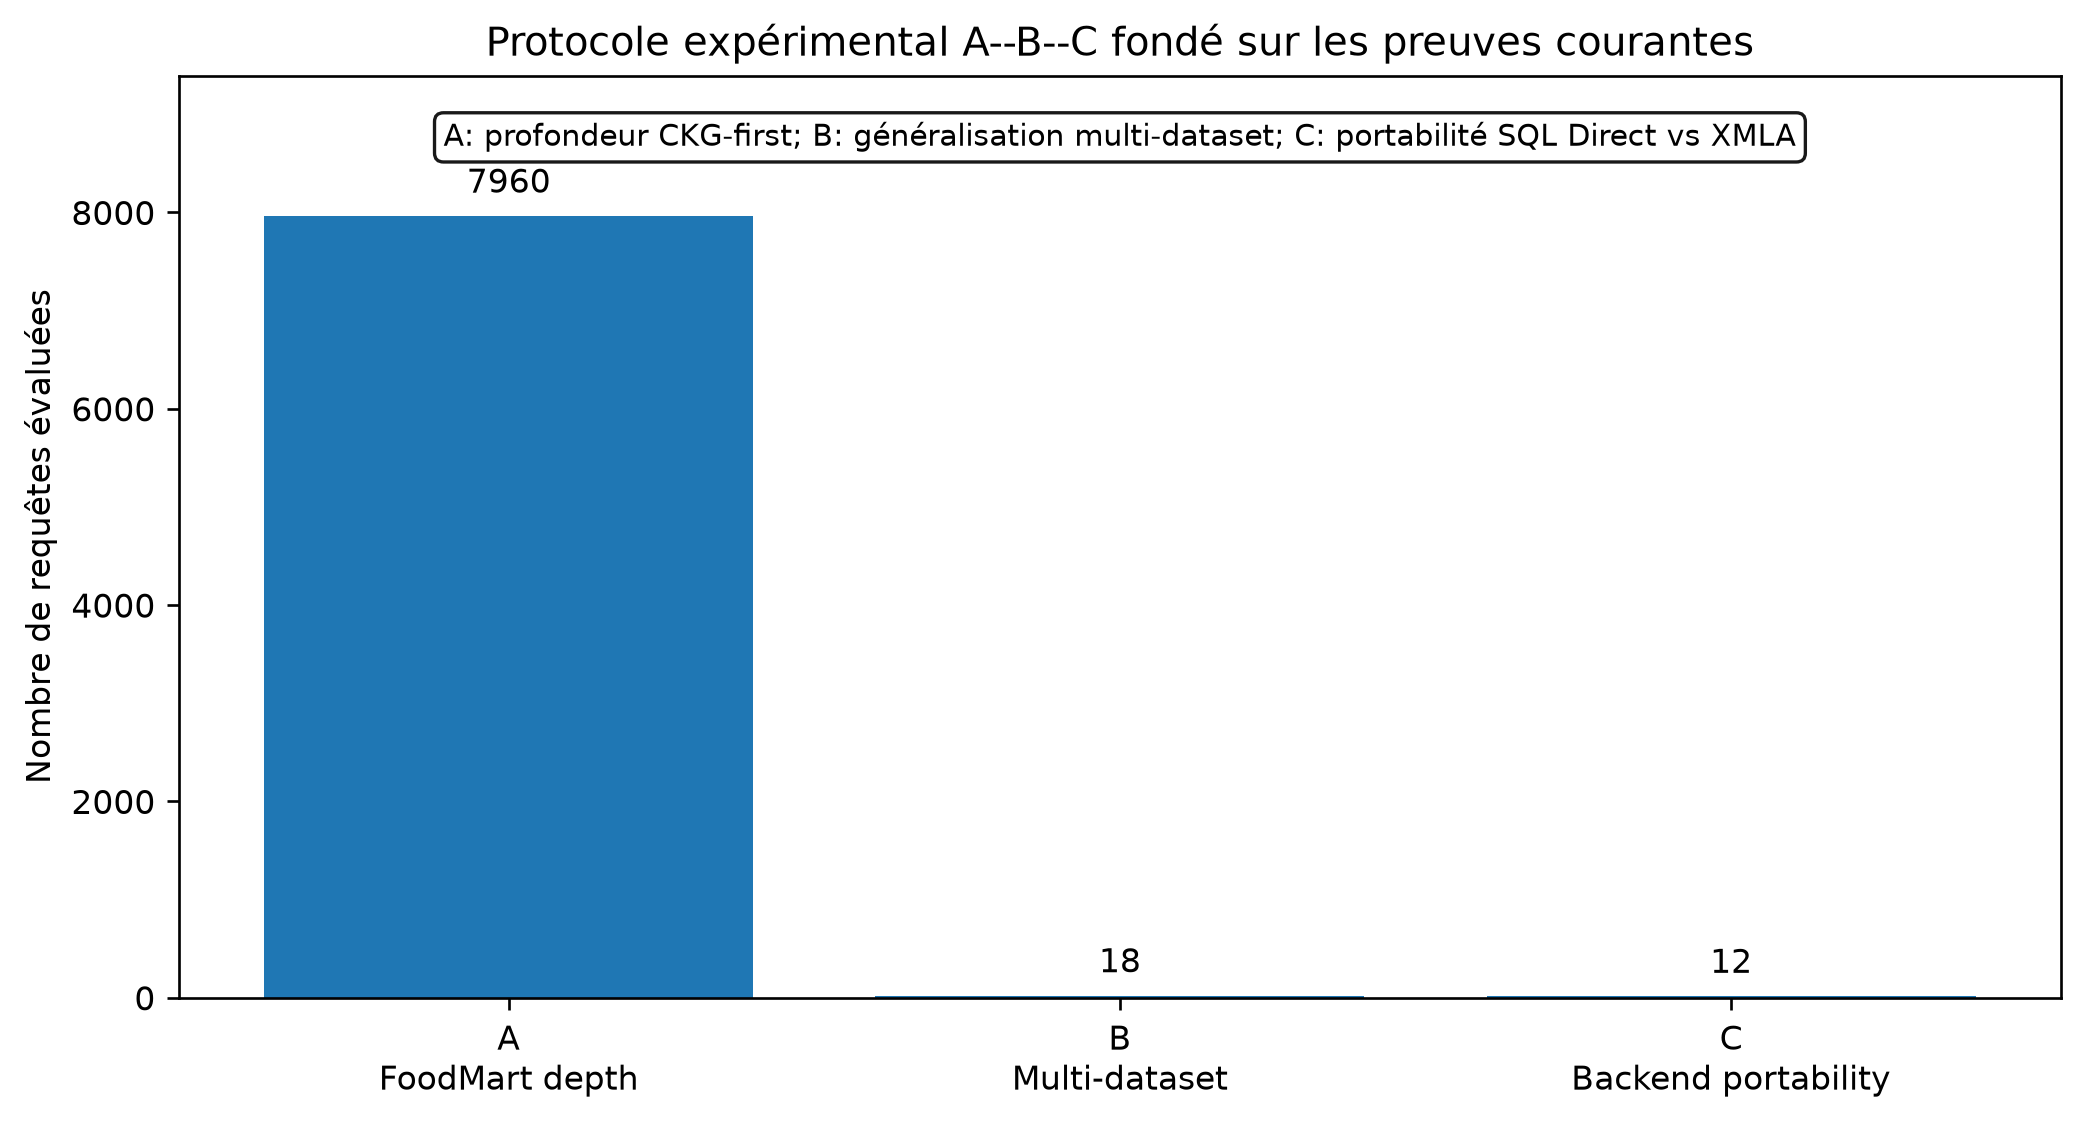
\includegraphics[width=\linewidth]{figures/exp_workflow_diagram.png}
\caption{Chaîne expérimentale reproductible utilisée pour reconstruire les sessions, décisions, preuves CKG, tableaux et figures de l'article.}
\label{fig:abc-workflow}
\end{figure}

\begin{figure}[t]
\centering
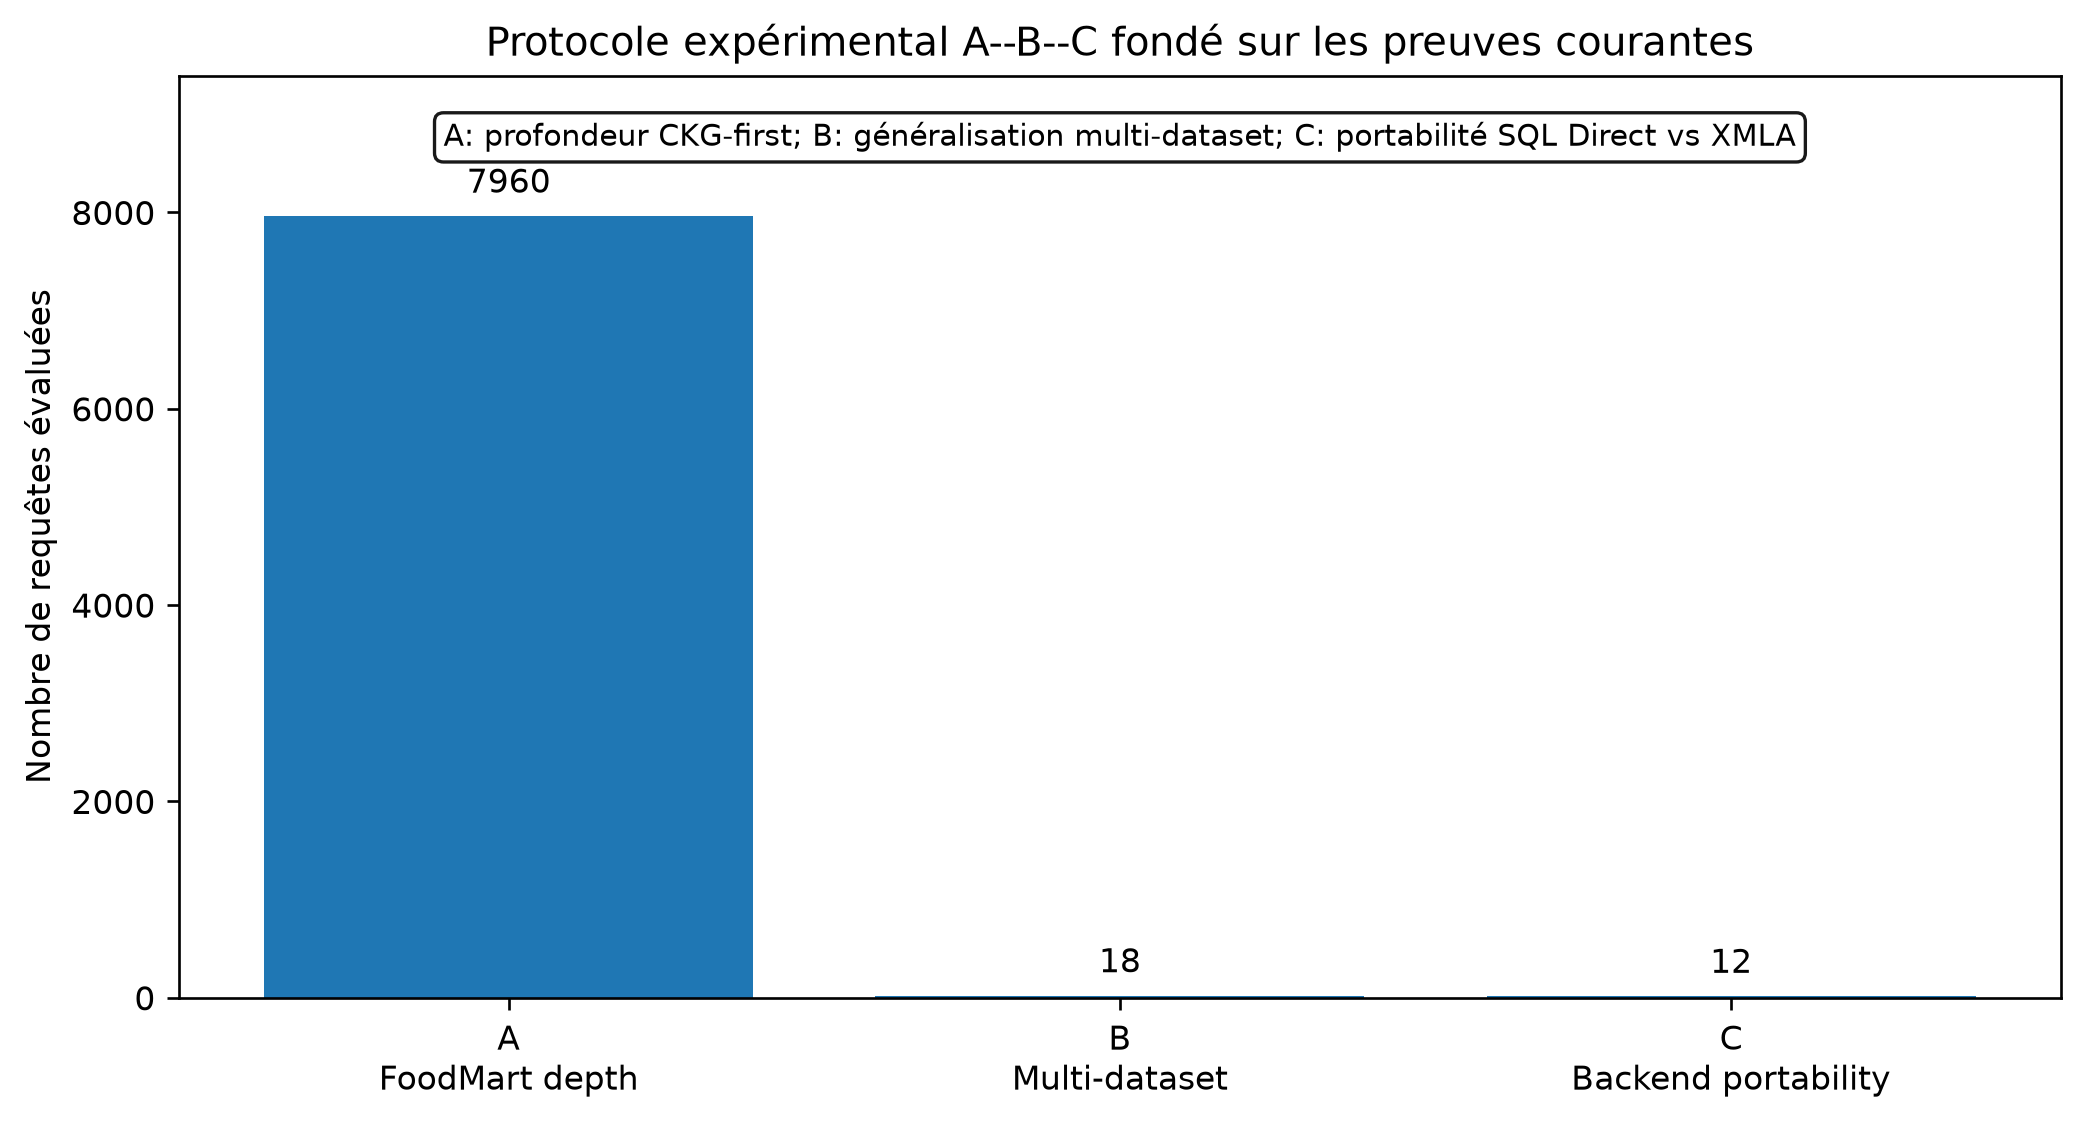
\includegraphics[width=\linewidth]{figures/fig_protocol_adopte.png}
\caption{Protocole adopté pour l'évaluation A--B--C : profondeur FoodMart, validation multi-dataset contrôlée et portabilité backend.}
\label{fig:abc-protocol}
\end{figure}

\subsection{Campagne A : profondeur expérimentale FoodMart}

La Campagne A constitue la campagne de profondeur. Elle exploite le snapshot FoodMart verrouillé afin d'évaluer la stabilité du mécanisme MCAD sur un volume important de sessions analytiques. Le snapshot verrouillé contient 2266 événements CKG utiles, correspondant aux contributions retenues après application du prédicat de validité contextuelle, de la réalisabilité, de la calculabilité et du filtrage par contribution marginale.

\begin{table*}[!t]
\centering
\caption{Résultats par campagne et par politique pour le benchmark article courant.}
\scriptsize
\setlength{\tabcolsep}{4pt}
\begin{tabular}{@{}lrrrrrrrr@{}}
\toprule
Campagne & Politique & Sessions & Requêtes & \$\textbackslash\{\}phi\_\{final\}\$ & False allow & False block & F1 block & p95 ms \\
\midrule
A\_core\_foodmart\_mcad\_gate & MCAD-Gate & 750 & 6000 & 0.9200 & 0.0000 & 0.0000 & 1.0000 & 0.2491 \\
A\_core\_foodmart\_mcad\_gate & Measure-overlap & 750 & 6000 & 0.9200 & 0.9297 & 0.0000 & 0.1314 & 0.1092 \\
A\_core\_foodmart\_mcad\_gate & Naïve & 750 & 6000 & 0.9200 & 1.0000 & 0.0000 & 0.0000 & 0.0788 \\
A\_core\_foodmart\_mcad\_gate & Random matched & 750 & 6000 & 0.2360 & 0.2184 & 0.7435 & 0.7802 & 0.0909 \\
B\_multidataset\_generalization & MCAD-Gate & 300 & 2400 & 0.9200 & 0.0000 & 0.0000 & 1.0000 & 0.2490 \\
B\_multidataset\_generalization & Measure-overlap & 300 & 2400 & 0.9200 & 0.9291 & 0.0000 & 0.1324 & 0.1088 \\
B\_multidataset\_generalization & Naïve & 300 & 2400 & 0.9200 & 1.0000 & 0.0000 & 0.0000 & 0.0791 \\
B\_multidataset\_generalization & Random matched & 300 & 2400 & 0.2467 & 0.2062 & 0.7319 & 0.7889 & 0.0923 \\
C\_backend\_portability & MCAD-Gate & 480 & 3840 & 0.9250 & 0.0000 & 0.0000 & 1.0000 & 0.2488 \\
\bottomrule
\end{tabular}
\normalsize
\label{tab:article-policy-summary}
\end{table*}


\begin{table*}[!t]
\centering
\caption{Résumé par dataset et politique pour le benchmark article courant.}
\scriptsize
\setlength{\tabcolsep}{4pt}
\begin{tabular}{@{}lrrrrrrr@{}}
\toprule
Campagne & Dataset & Politique & Sessions & \$\textbackslash\{\}phi\_\{final\}\$ & False allow & Exec. non contrib. & p95 ms \\
\midrule
A\_core\_foodmart\_mcad\_gate & FoodMart & MCAD-Gate & 750 & 0.9200 & 0.0000 & 0.0000 & 0.2491 \\
A\_core\_foodmart\_mcad\_gate & FoodMart & Measure-overlap & 750 & 0.9200 & 0.9297 & 0.7568 & 0.1092 \\
A\_core\_foodmart\_mcad\_gate & FoodMart & Naïve & 750 & 0.9200 & 1.0000 & 0.7700 & 0.0788 \\
A\_core\_foodmart\_mcad\_gate & FoodMart & Random matched & 750 & 0.2360 & 0.2184 & 0.7403 & 0.0909 \\
B\_multidataset\_generalization & AdventureWorksDW & MCAD-Gate & 100 & 0.9200 & 0.0000 & 0.0000 & 0.2485 \\
B\_multidataset\_generalization & AdventureWorksDW & Measure-overlap & 100 & 0.9200 & 0.9318 & 0.7573 & 0.1083 \\
B\_multidataset\_generalization & AdventureWorksDW & Naïve & 100 & 0.9200 & 1.0000 & 0.7700 & 0.0785 \\
B\_multidataset\_generalization & AdventureWorksDW & Random matched & 100 & 0.2500 & 0.1948 & 0.7059 & 0.0905 \\
B\_multidataset\_generalization & FoodMart & MCAD-Gate & 100 & 0.9200 & 0.0000 & 0.0000 & 0.2490 \\
B\_multidataset\_generalization & FoodMart & Measure-overlap & 100 & 0.9200 & 0.9286 & 0.7566 & 0.1086 \\
B\_multidataset\_generalization & FoodMart & Naïve & 100 & 0.9200 & 1.0000 & 0.7700 & 0.0791 \\
B\_multidataset\_generalization & FoodMart & Random matched & 100 & 0.2600 & 0.2354 & 0.7360 & 0.0908 \\
B\_multidataset\_generalization & SteelWheels & MCAD-Gate & 100 & 0.9200 & 0.0000 & 0.0000 & 0.2491 \\
B\_multidataset\_generalization & SteelWheels & Measure-overlap & 100 & 0.9200 & 0.9269 & 0.7563 & 0.1092 \\
B\_multidataset\_generalization & SteelWheels & Naïve & 100 & 0.9200 & 1.0000 & 0.7700 & 0.0791 \\
B\_multidataset\_generalization & SteelWheels & Random matched & 100 & 0.2300 & 0.1883 & 0.7160 & 0.0966 \\
C\_backend\_portability & AdventureWorksDW & MCAD-Gate & 240 & 0.9250 & 0.0000 & 0.0000 & 0.2486 \\
C\_backend\_portability & SteelWheels & MCAD-Gate & 240 & 0.9250 & 0.0000 & 0.0000 & 0.2491 \\
\bottomrule
\end{tabular}
\normalsize
\label{tab:dataset-results}
\end{table*}


\begin{table}[!t]
\centering
\caption{Distribution des raisons de décision dans la Campagne A FoodMart.}
\scriptsize
\setlength{\tabcolsep}{4pt}
\begin{tabular}{@{}lr@{}}
\toprule
Raison & Occurrences \\
\midrule
ALLOW\_NEW\_TOTAL & 2266 \\
BLOCK\_EMPTY\_SUBSPACE & 576 \\
BLOCK\_GRAIN\_MISMATCH & 770 \\
BLOCK\_MEASURE\_NOT\_TARGETED & 110 \\
BLOCK\_OUT\_OF\_OBJECTIVE\_SCOPE & 300 \\
BLOCK\_REDUNDANT\_DPHI\_ZERO & 3372 \\
BLOCK\_SLICER\_MISMATCH & 566 \\
\bottomrule
\end{tabular}
\normalsize
\label{tab:campaign-a-reasons}
\end{table}


\begin{figure}[t]
\centering
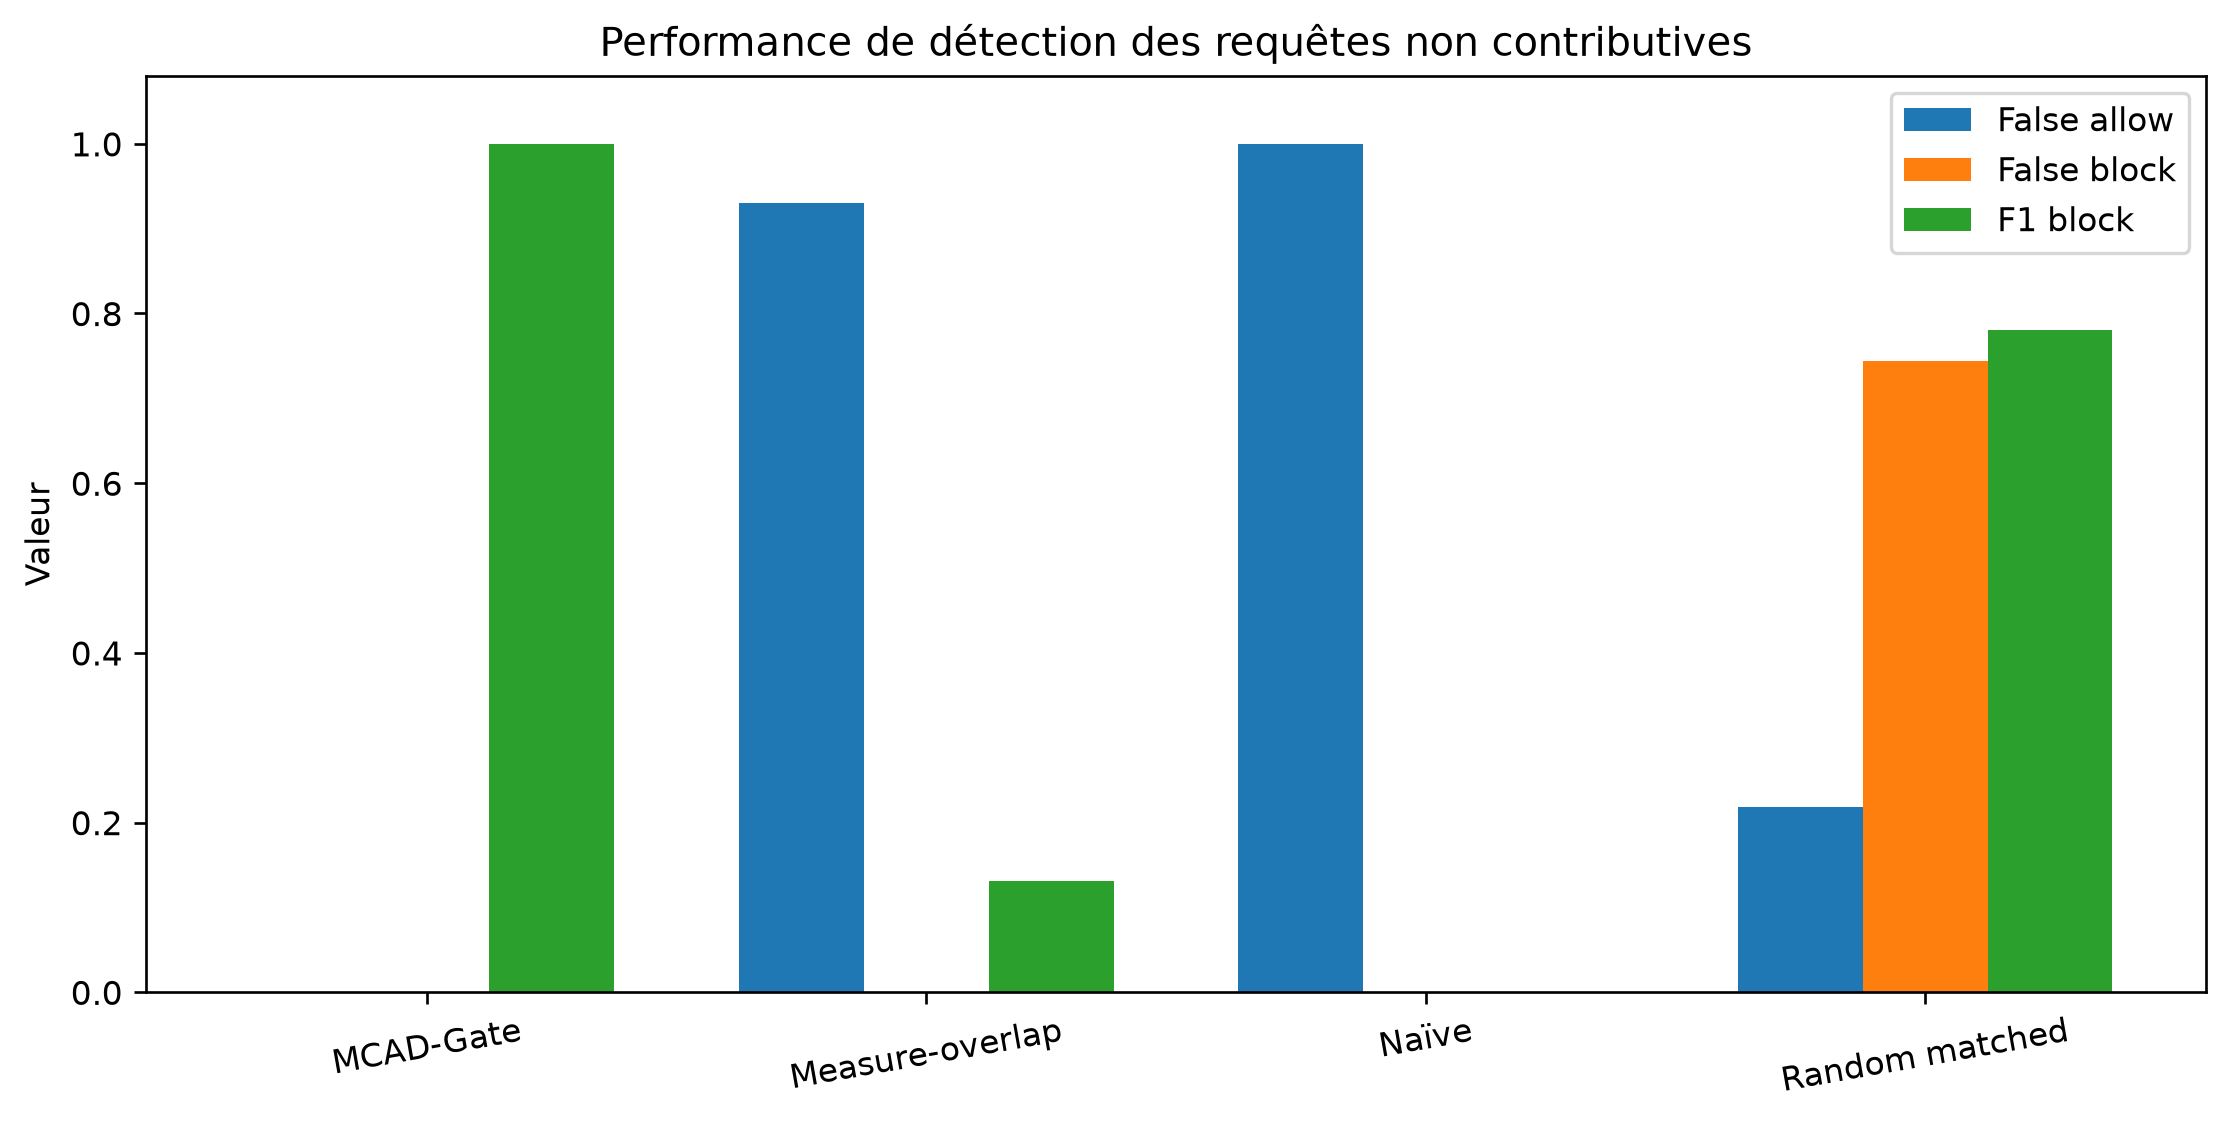
\includegraphics[width=\linewidth]{figures/fig_detection_performance.png}
\caption{Performance de détection : MCAD conserve les requêtes contributives tout en supprimant les exécutions non contributives et les false allows.}
\label{fig:detection-performance}
\end{figure}

\begin{figure}[t]
\centering
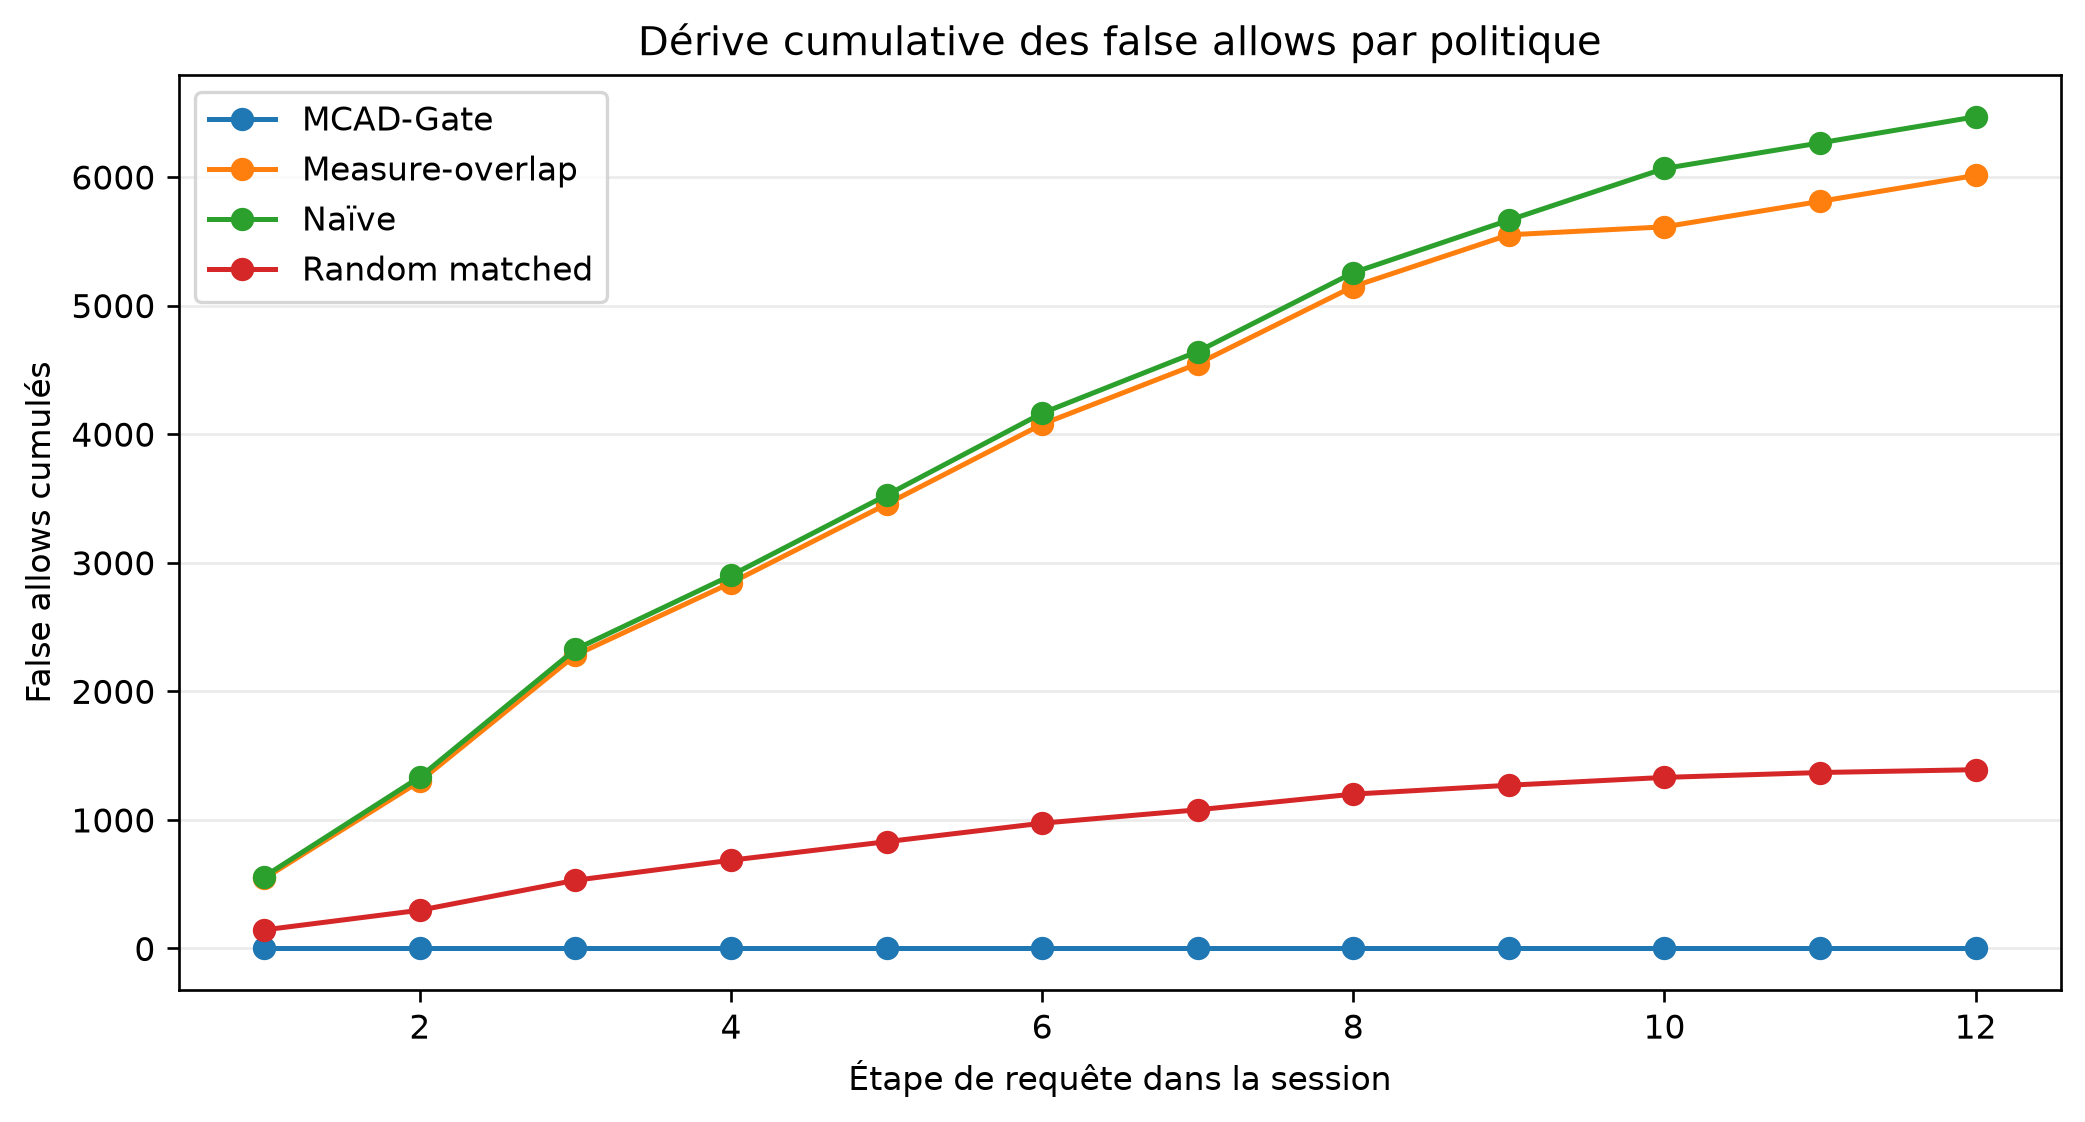
\includegraphics[width=\linewidth]{figures/false_allow_curve_by_step.png}
\caption{Évolution cumulée des false allows par étape de session. Les politiques permissives dérivent rapidement, tandis que MCAD maintient une sélectivité stricte.}
\label{fig:false-allow-curve}
\end{figure}

\begin{figure}[t]
\centering
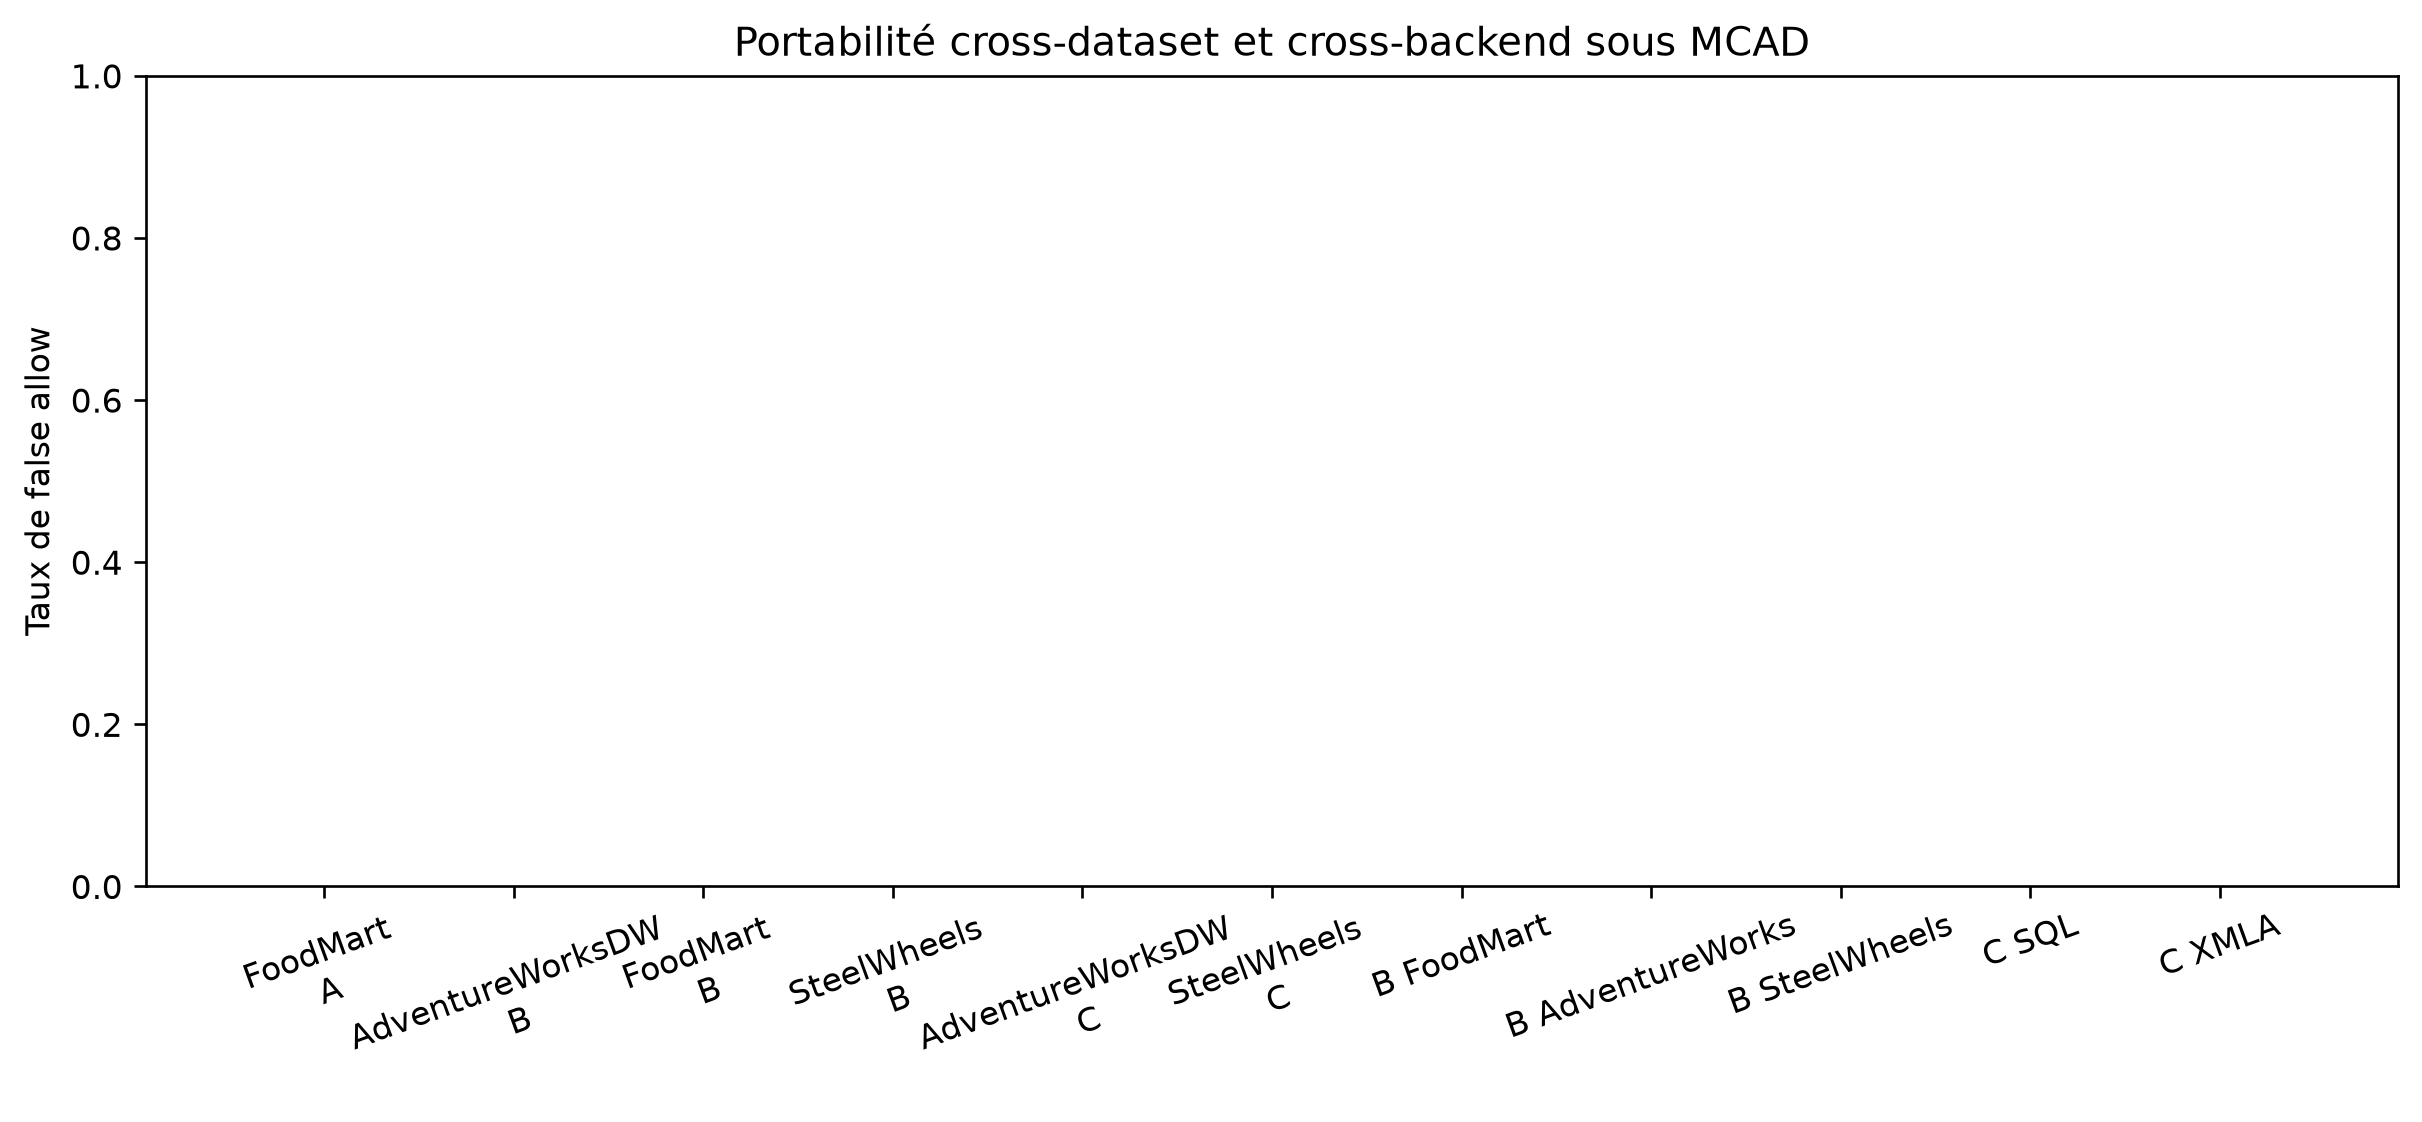
\includegraphics[width=\linewidth]{figures/dataset_false_allow_portability.png}
\caption{Taux de false allow par dataset et signal de portabilité de la politique MCAD.}
\label{fig:dataset-false-allow-portability}
\end{figure}

\subsection{Robustesse, ablations et explicabilité des blocages}

La robustesse est évaluée au moyen de charges analytiques incluant des requêtes contributives, des requêtes bruitées, des violations de grain, des incompatibilités de slicers, des mesures non ciblées et des requêtes redondantes. L'objectif est de vérifier que MCAD ne bloque pas arbitrairement, mais qu'il produit des décisions explicables par des raisons liées au CKG et à la chaîne QP $\rightarrow$ SAT $\rightarrow$ Real $\rightarrow$ Ceval $\rightarrow$ $\phi$.

\begin{figure}[t]
\centering
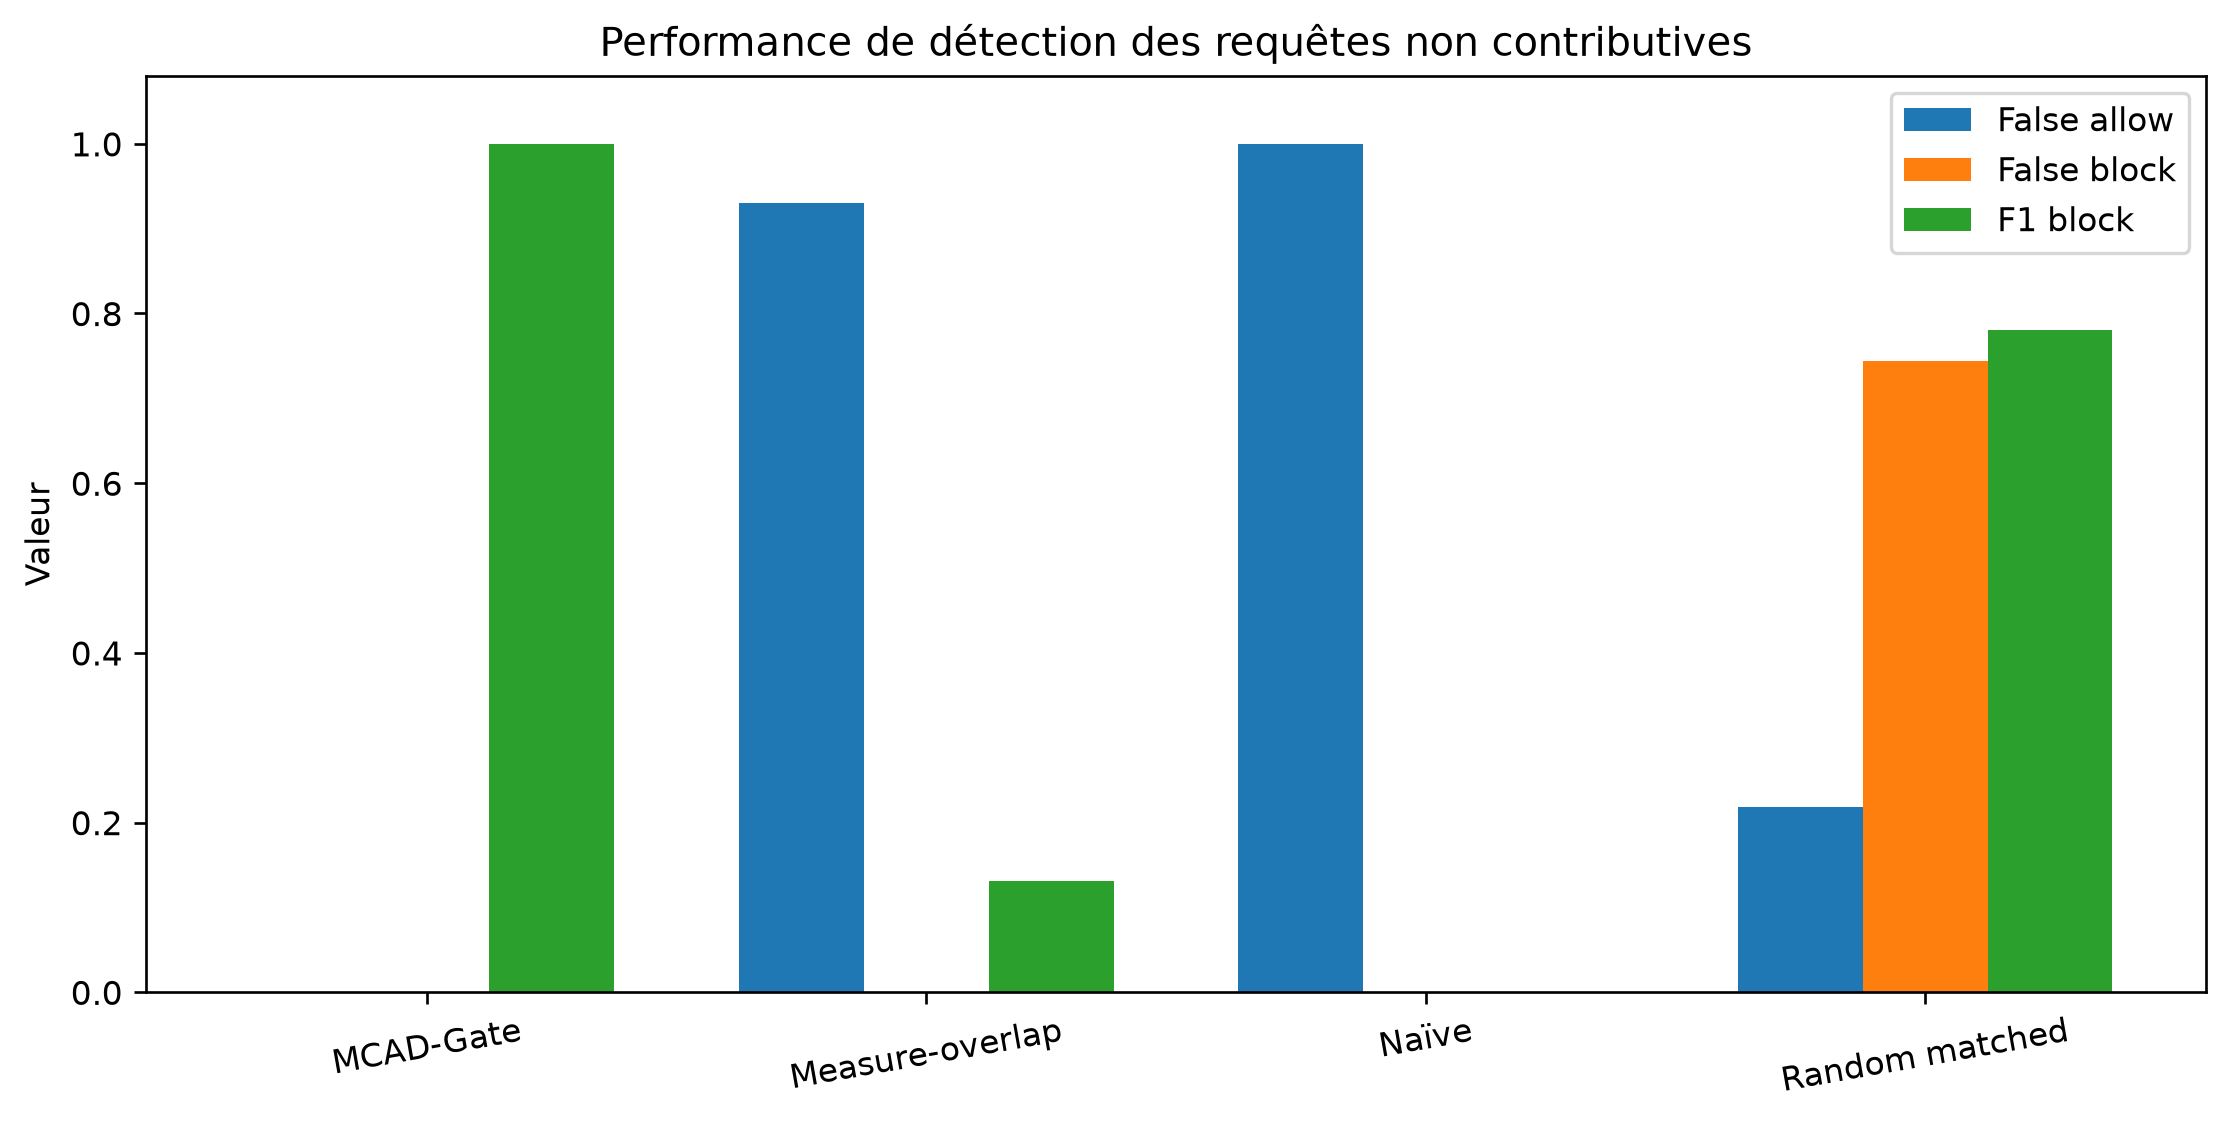
\includegraphics[width=\linewidth]{figures/robustness_false_allow_by_policy.png}
\caption{Robustesse face aux charges bruitées et adversariales : comparaison du taux de false allow par politique.}
\label{fig:robustness-false-allow}
\end{figure}

\begin{figure}[t]
\centering
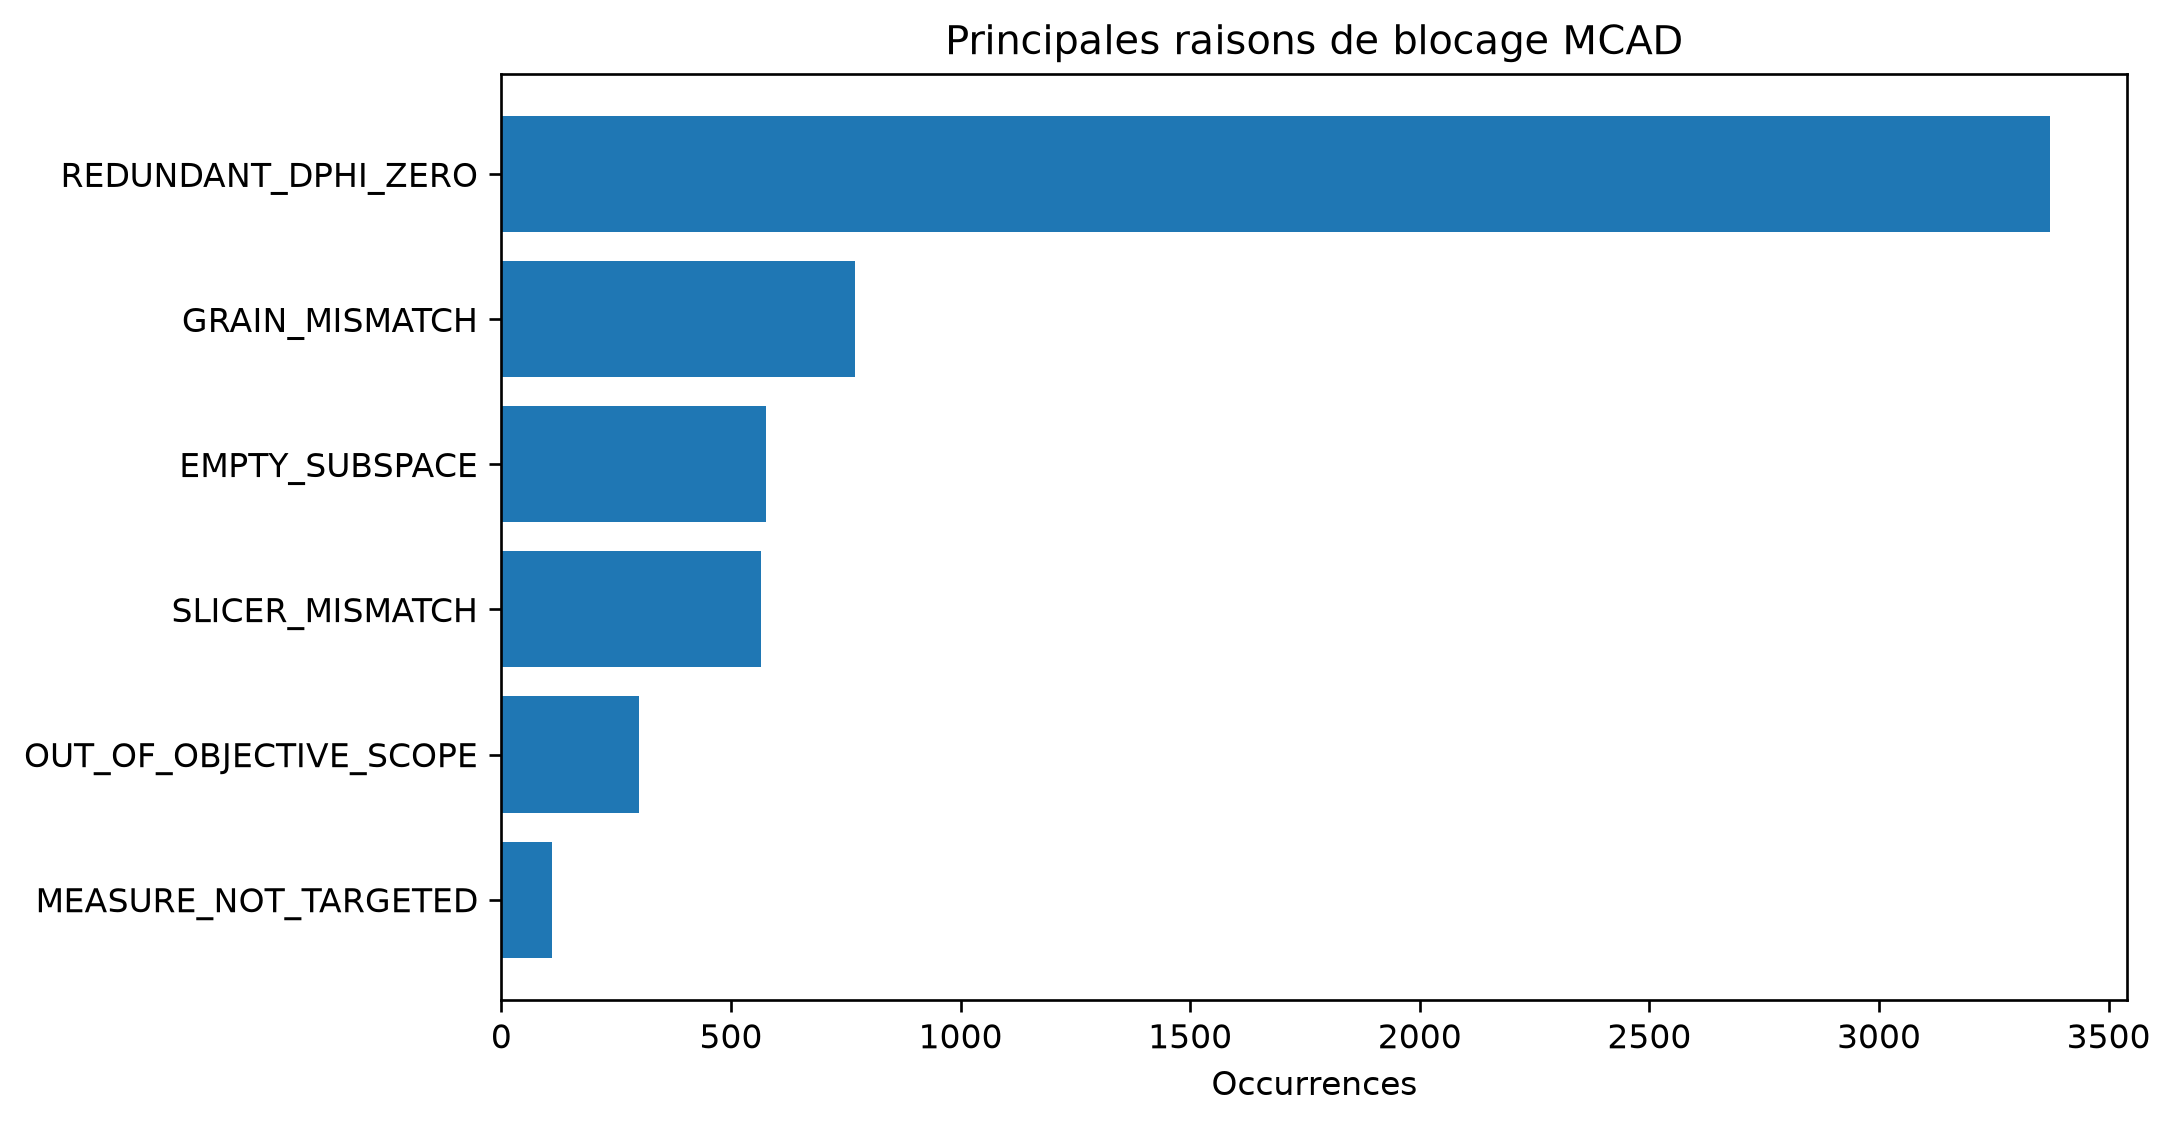
\includegraphics[width=\linewidth]{figures/robustness_block_reason_distribution_mcad.png}
\caption{Distribution des principales raisons de blocage sous MCAD. Les blocages sont rattachés à des violations ou insuffisances interprétables.}
\label{fig:block-reason-distribution}
\end{figure}

\begin{figure}[t]
\centering
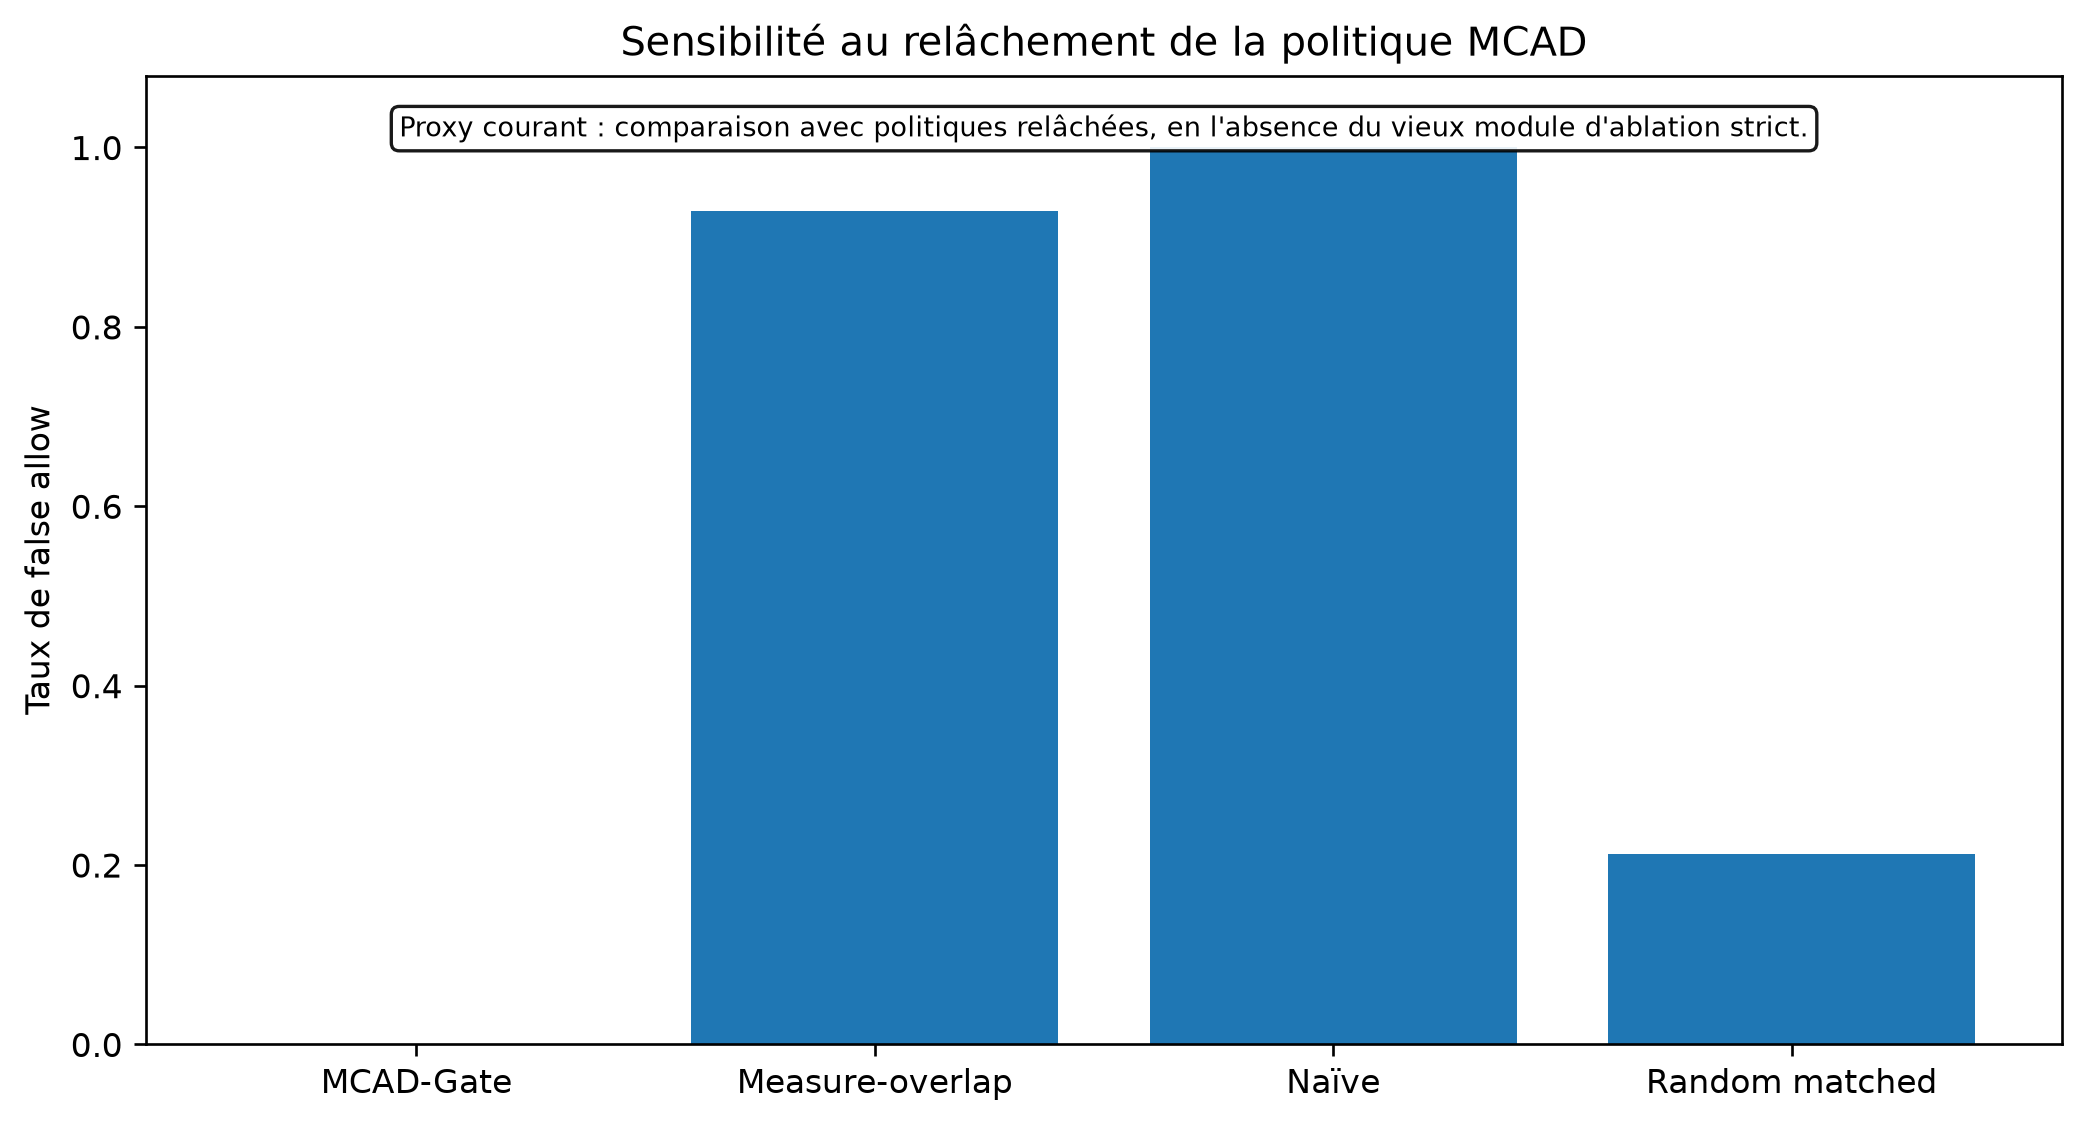
\includegraphics[width=\linewidth]{figures/ablation_sensitivity_false_allow.png}
\caption{Analyse d'ablation : sensibilité du taux de false allow lorsque certains composants de la chaîne formelle sont affaiblis.}
\label{fig:ablation-sensitivity}
\end{figure}

\subsection{Scalabilité et contrôle de croissance du CKG}

La scalabilité est évaluée en faisant croître le nombre d'objectifs, de contraintes, de nœuds virtuels et d'événements de session. Les résultats visent à distinguer le coût du chemin de décision en ligne du coût de persistance et d'archivage du graphe. Cette distinction est importante, car MCAD doit rester compatible avec un usage interactif, même si le CKG croît au fil des sessions.

\begin{figure}[t]
\centering
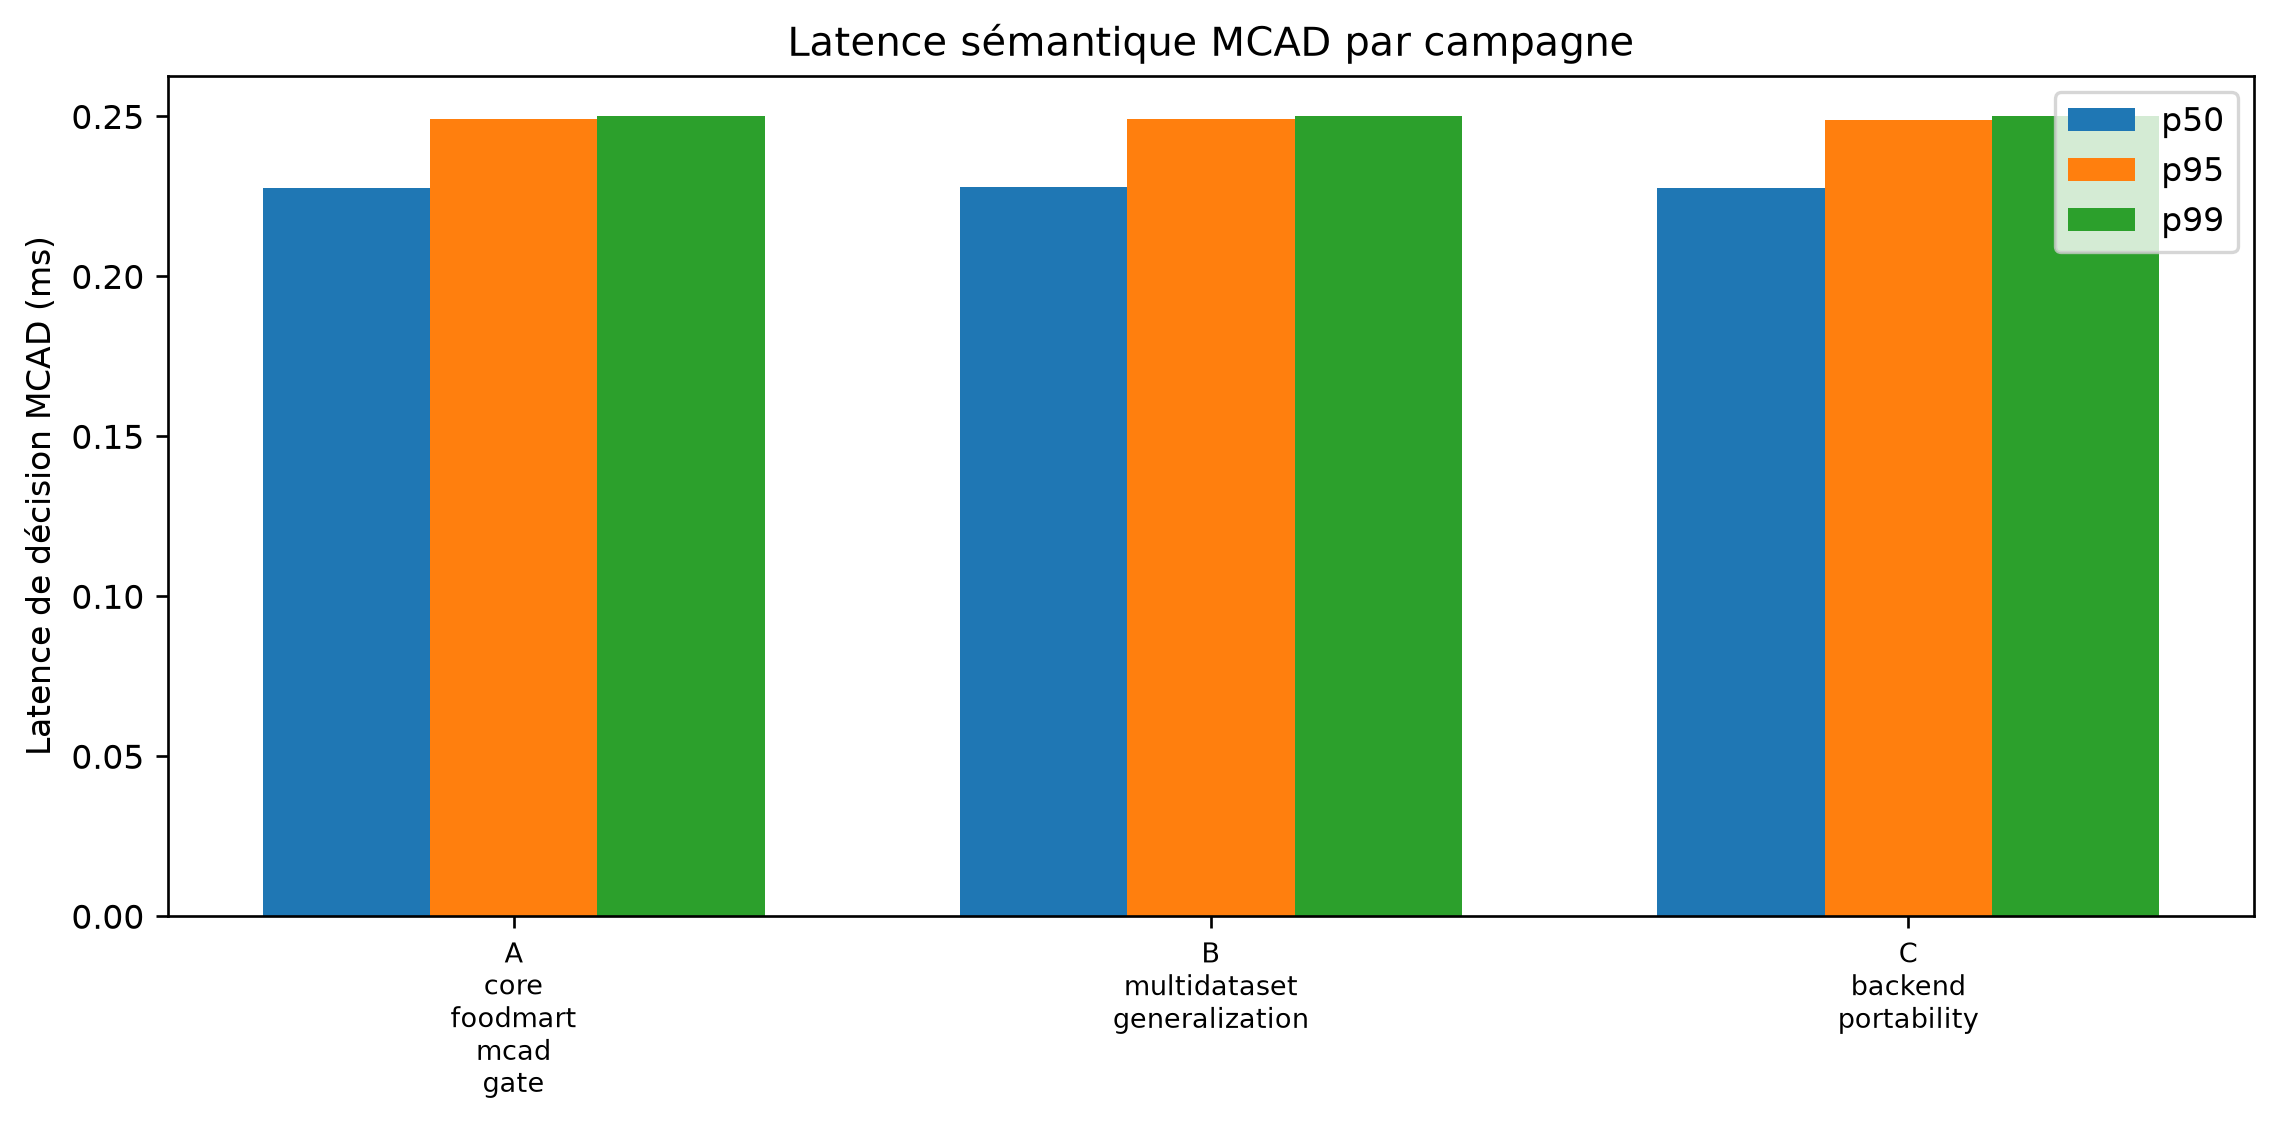
\includegraphics[width=\linewidth]{figures/scalability_latency_vs_nvs.png}
\caption{Latence d'évaluation en fonction de la taille du modèle d'objectif et du nombre de nœuds virtuels.}
\label{fig:scalability-latency}
\end{figure}

\begin{figure}[t]
\centering
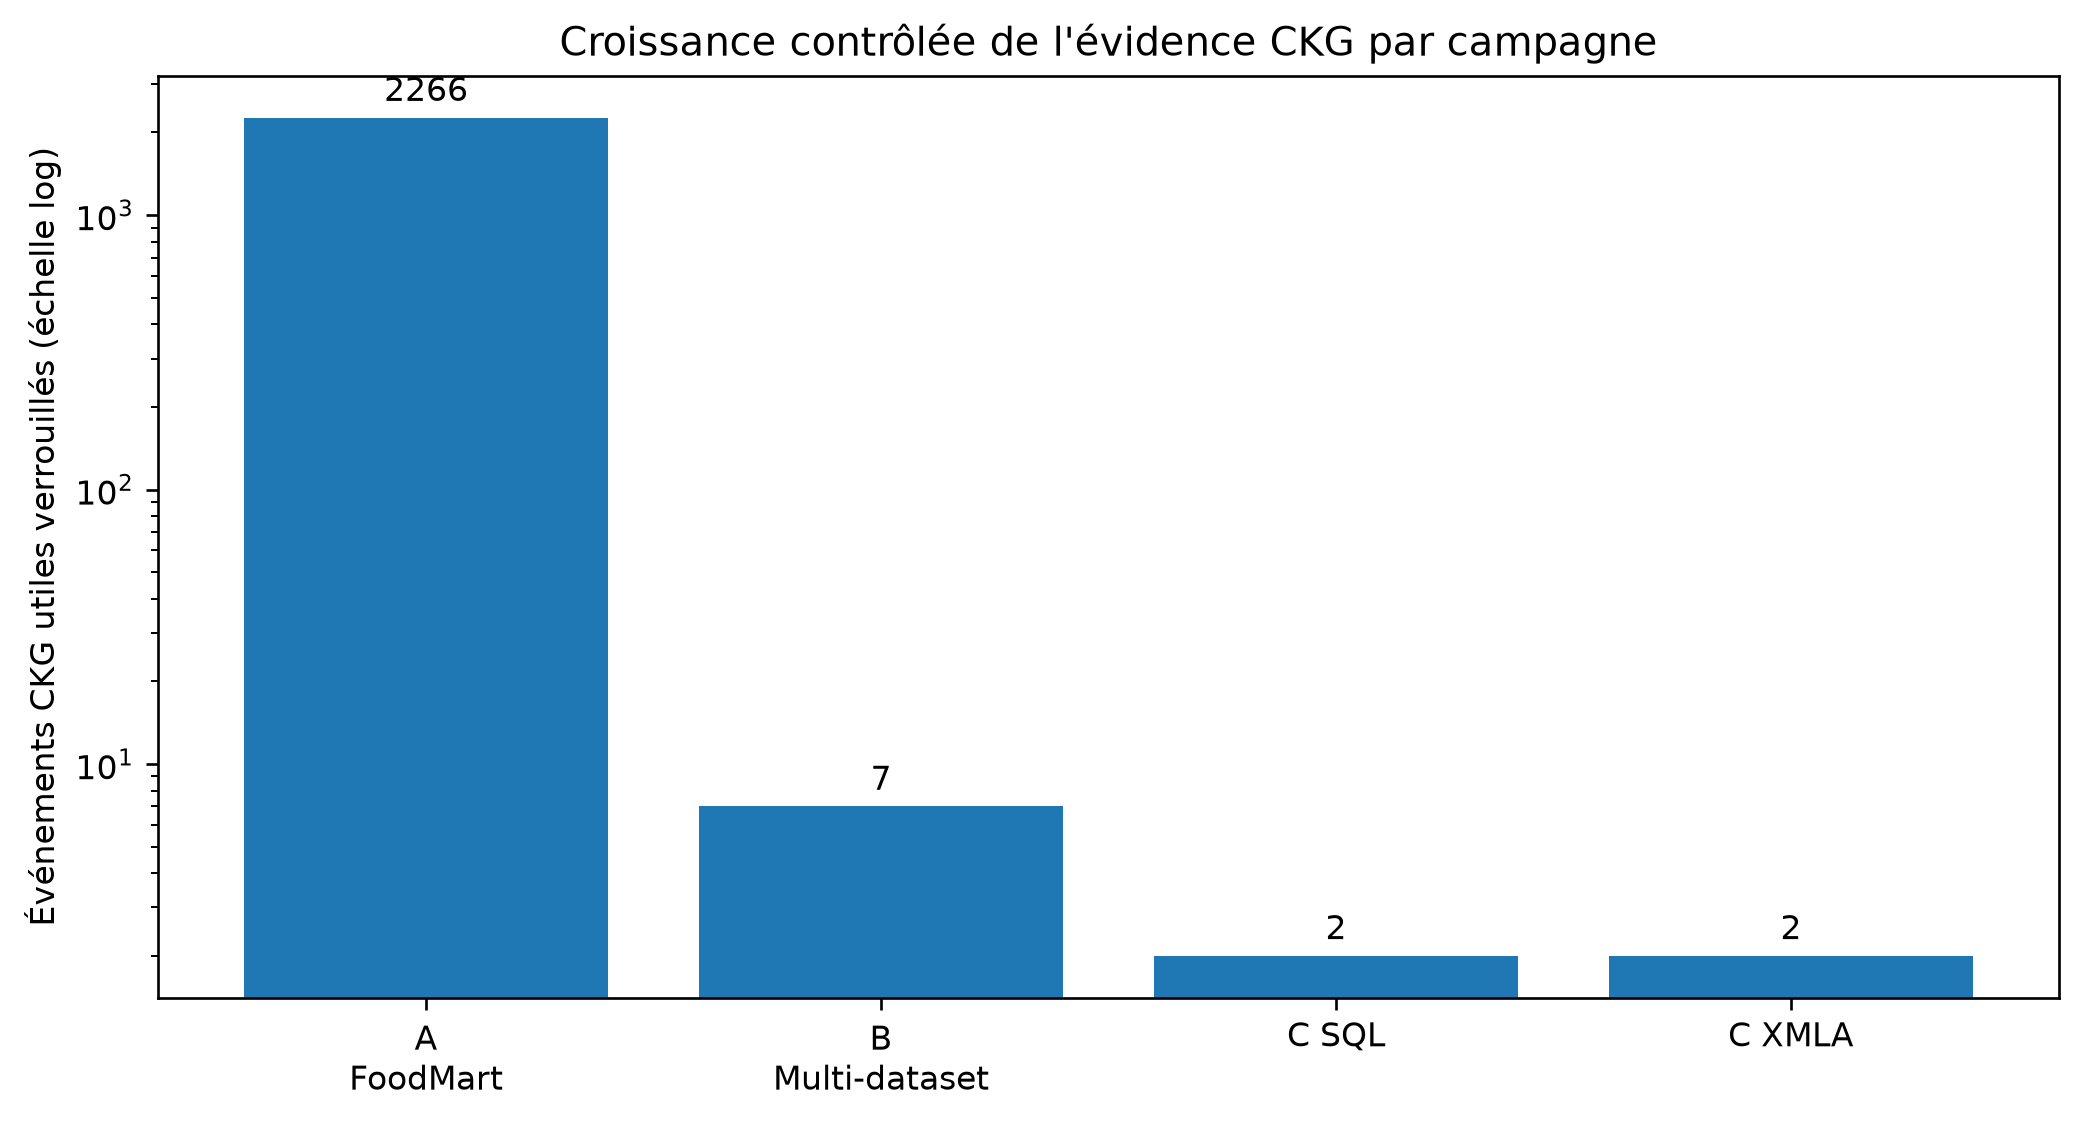
\includegraphics[width=\linewidth]{figures/ckg_growth_control_nodes.png}
\caption{Contrôle de croissance du CKG runtime : comparaison entre accumulation brute et compaction session-locale.}
\label{fig:ckg-growth-control}
\end{figure}

\begin{figure}[t]
\centering
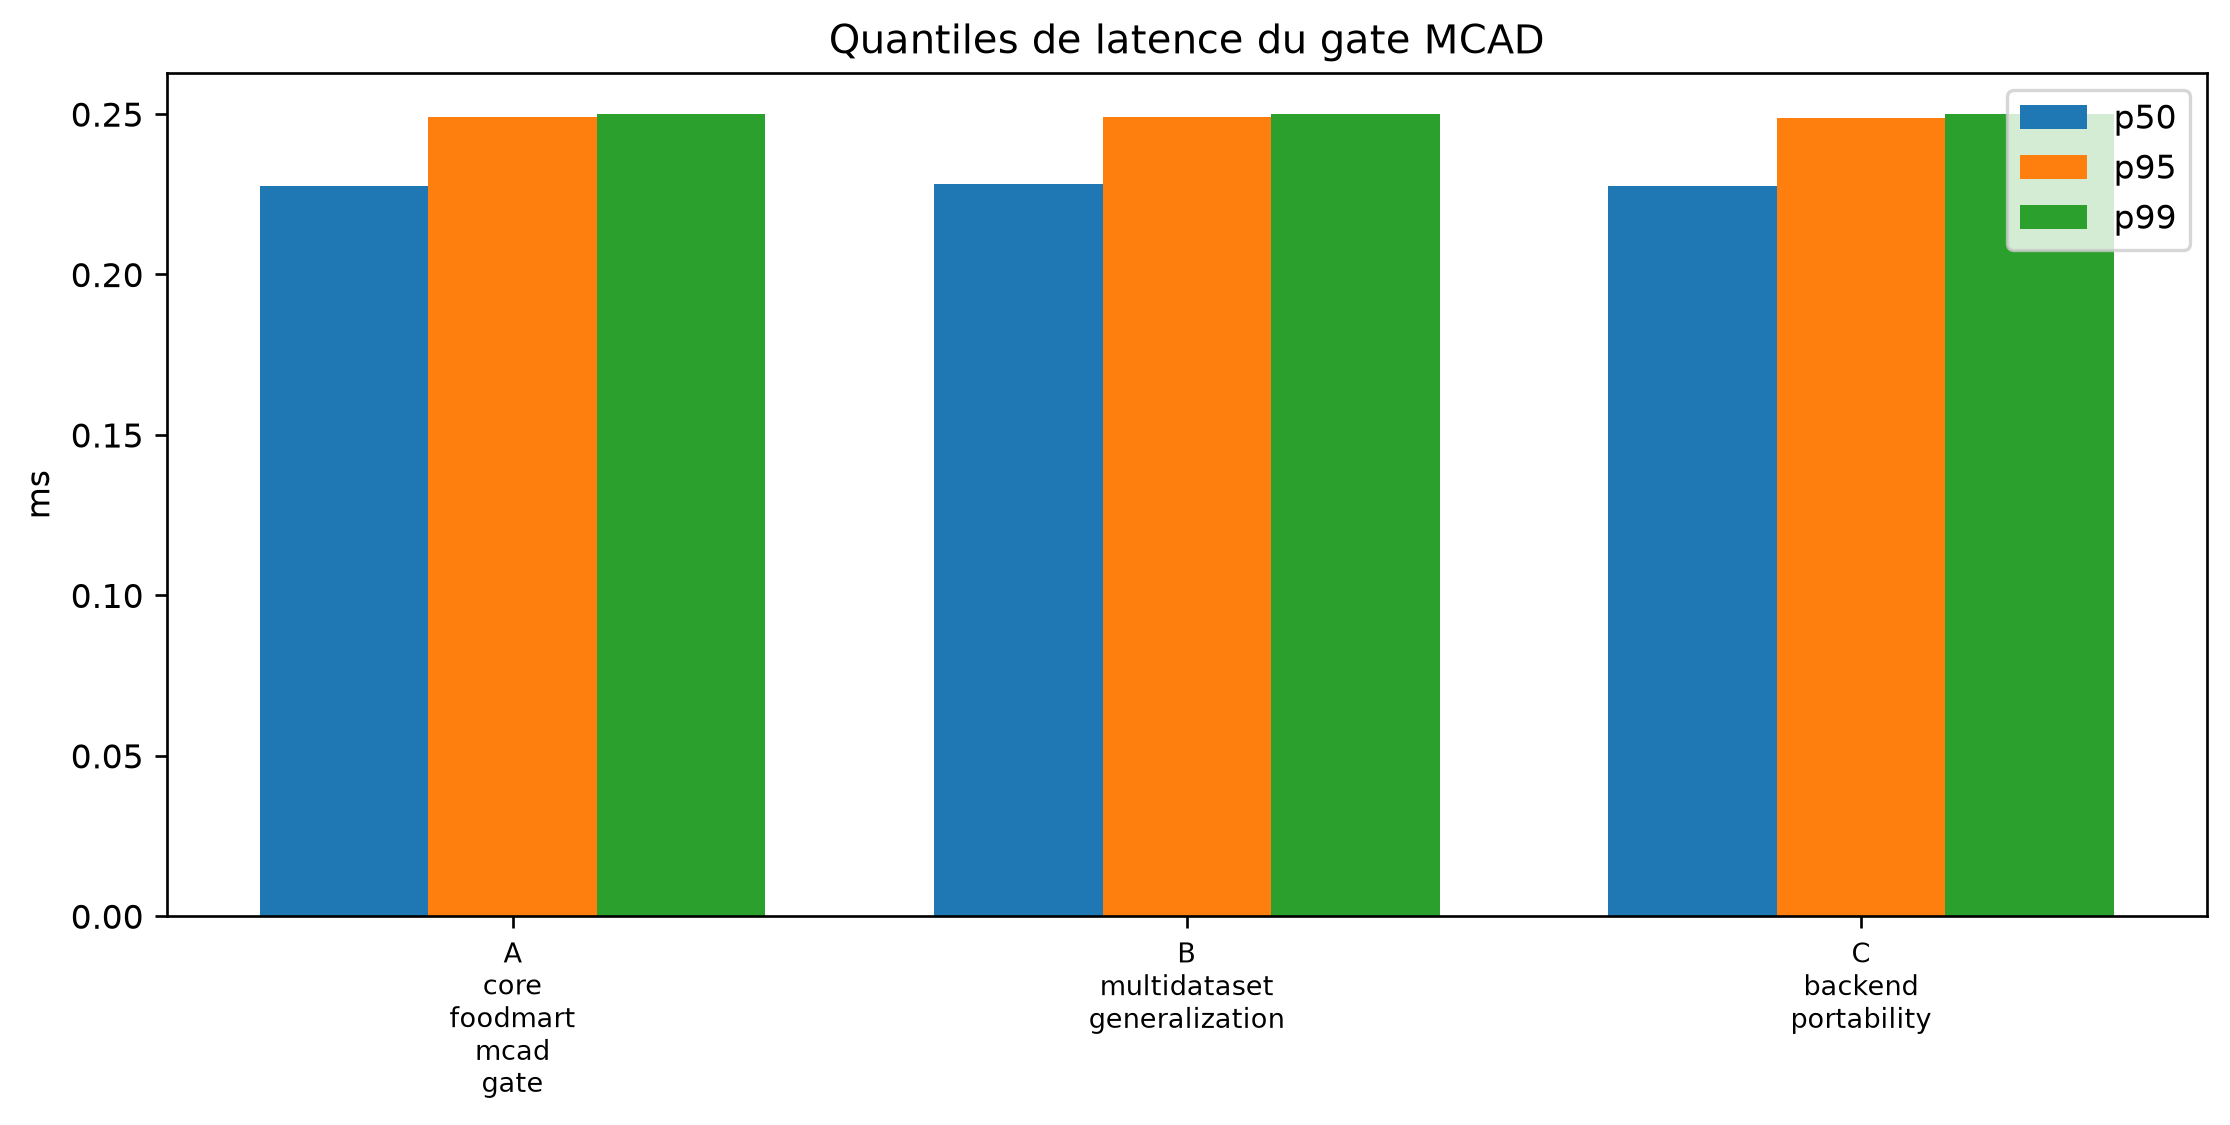
\includegraphics[width=\linewidth]{figures/runtime_latency_quantiles.png}
\caption{Quantiles de latence runtime observés pendant l'évaluation.}
\label{fig:runtime-latency}
\end{figure}

\subsection{Utilité de l'évidence et validation humaine}

La couche d'évidence CKG est évaluée comme une mémoire utile, persistée et réutilisable. Une requête autorisée ne produit pas seulement un résultat analytique : elle crée une trace utile de contribution, liée à la session, à l'objectif, au backend et à la partie de l'objectif rendue calculable. Cette propriété permet d'amorcer des sessions ultérieures et de réduire le nombre d'étapes nécessaires pour retrouver une couverture complète.

\begin{figure}[t]
\centering
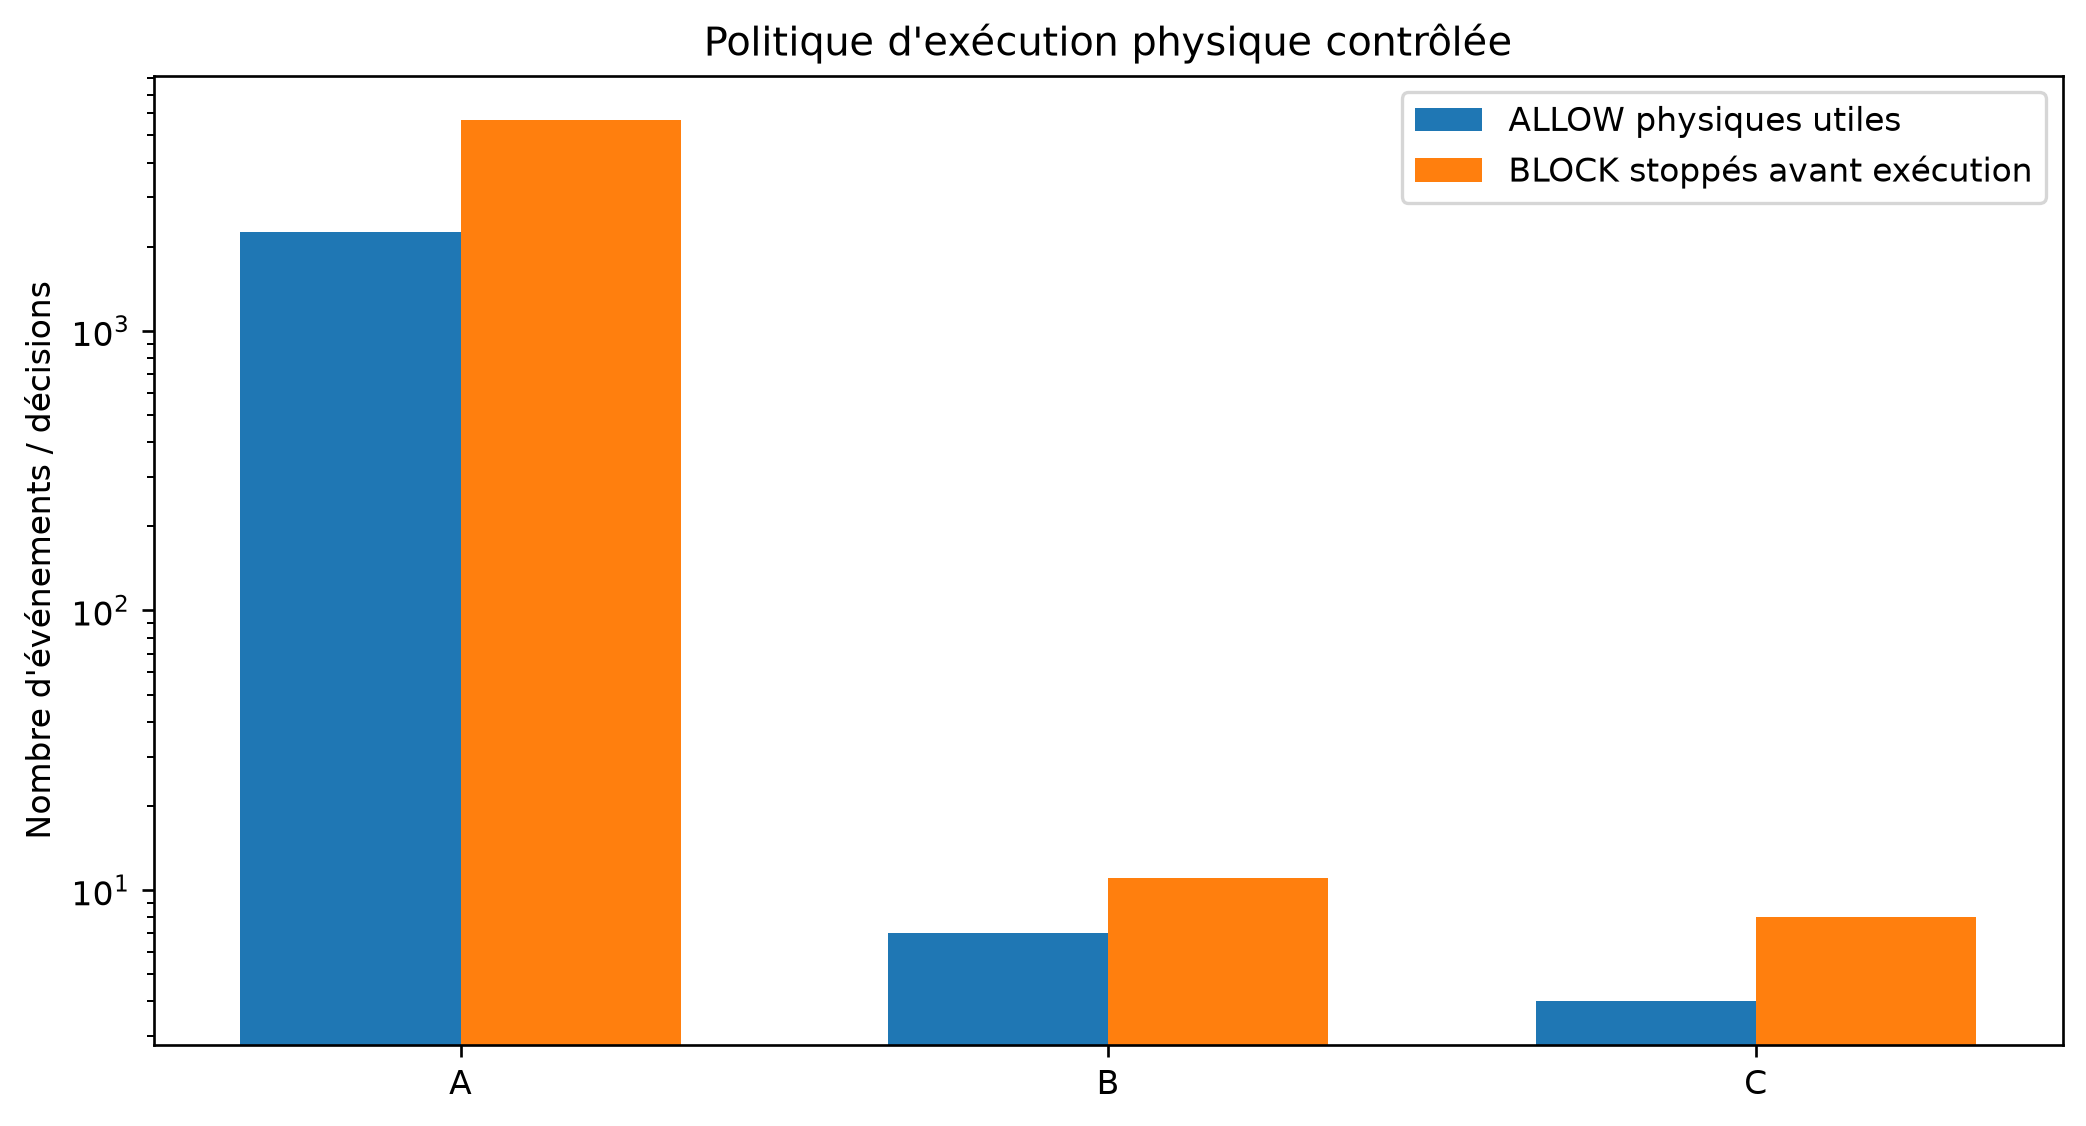
\includegraphics[width=\linewidth]{figures/evidence_usefulness_summary.png}
\caption{Utilité pratique de l'évidence CKG retenue : couverture initiale, réutilisation et réduction des étapes nécessaires.}
\label{fig:evidence-usefulness}
\end{figure}

\begin{figure}[t]
\centering
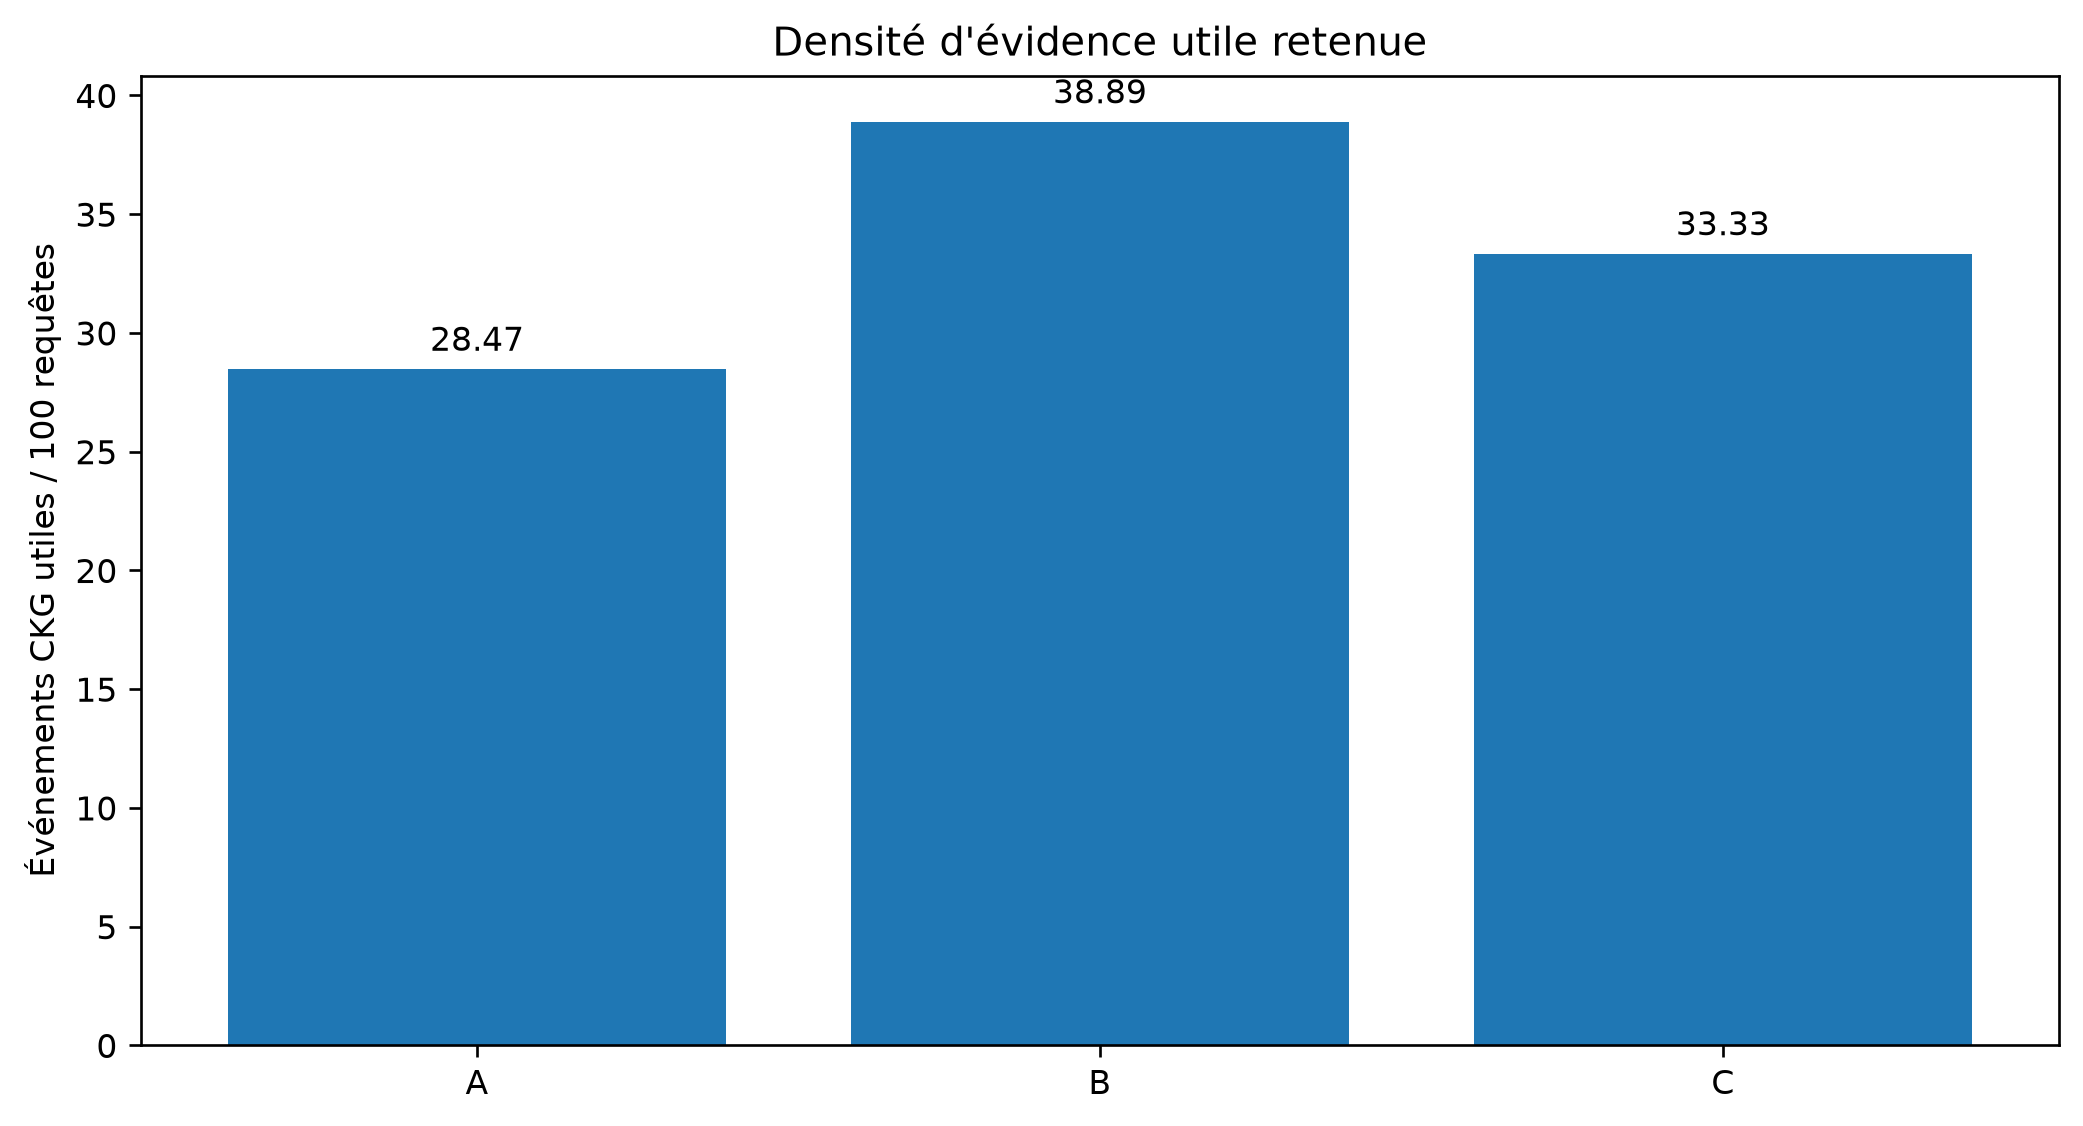
\includegraphics[width=\linewidth]{figures/evidence_bootstrap_steps_to_full.png}
\caption{Analyse bootstrap du nombre d'étapes nécessaires pour atteindre une couverture complète avec et sans évidence réutilisée.}
\label{fig:evidence-bootstrap}
\end{figure}

\begin{figure}[t]
\centering
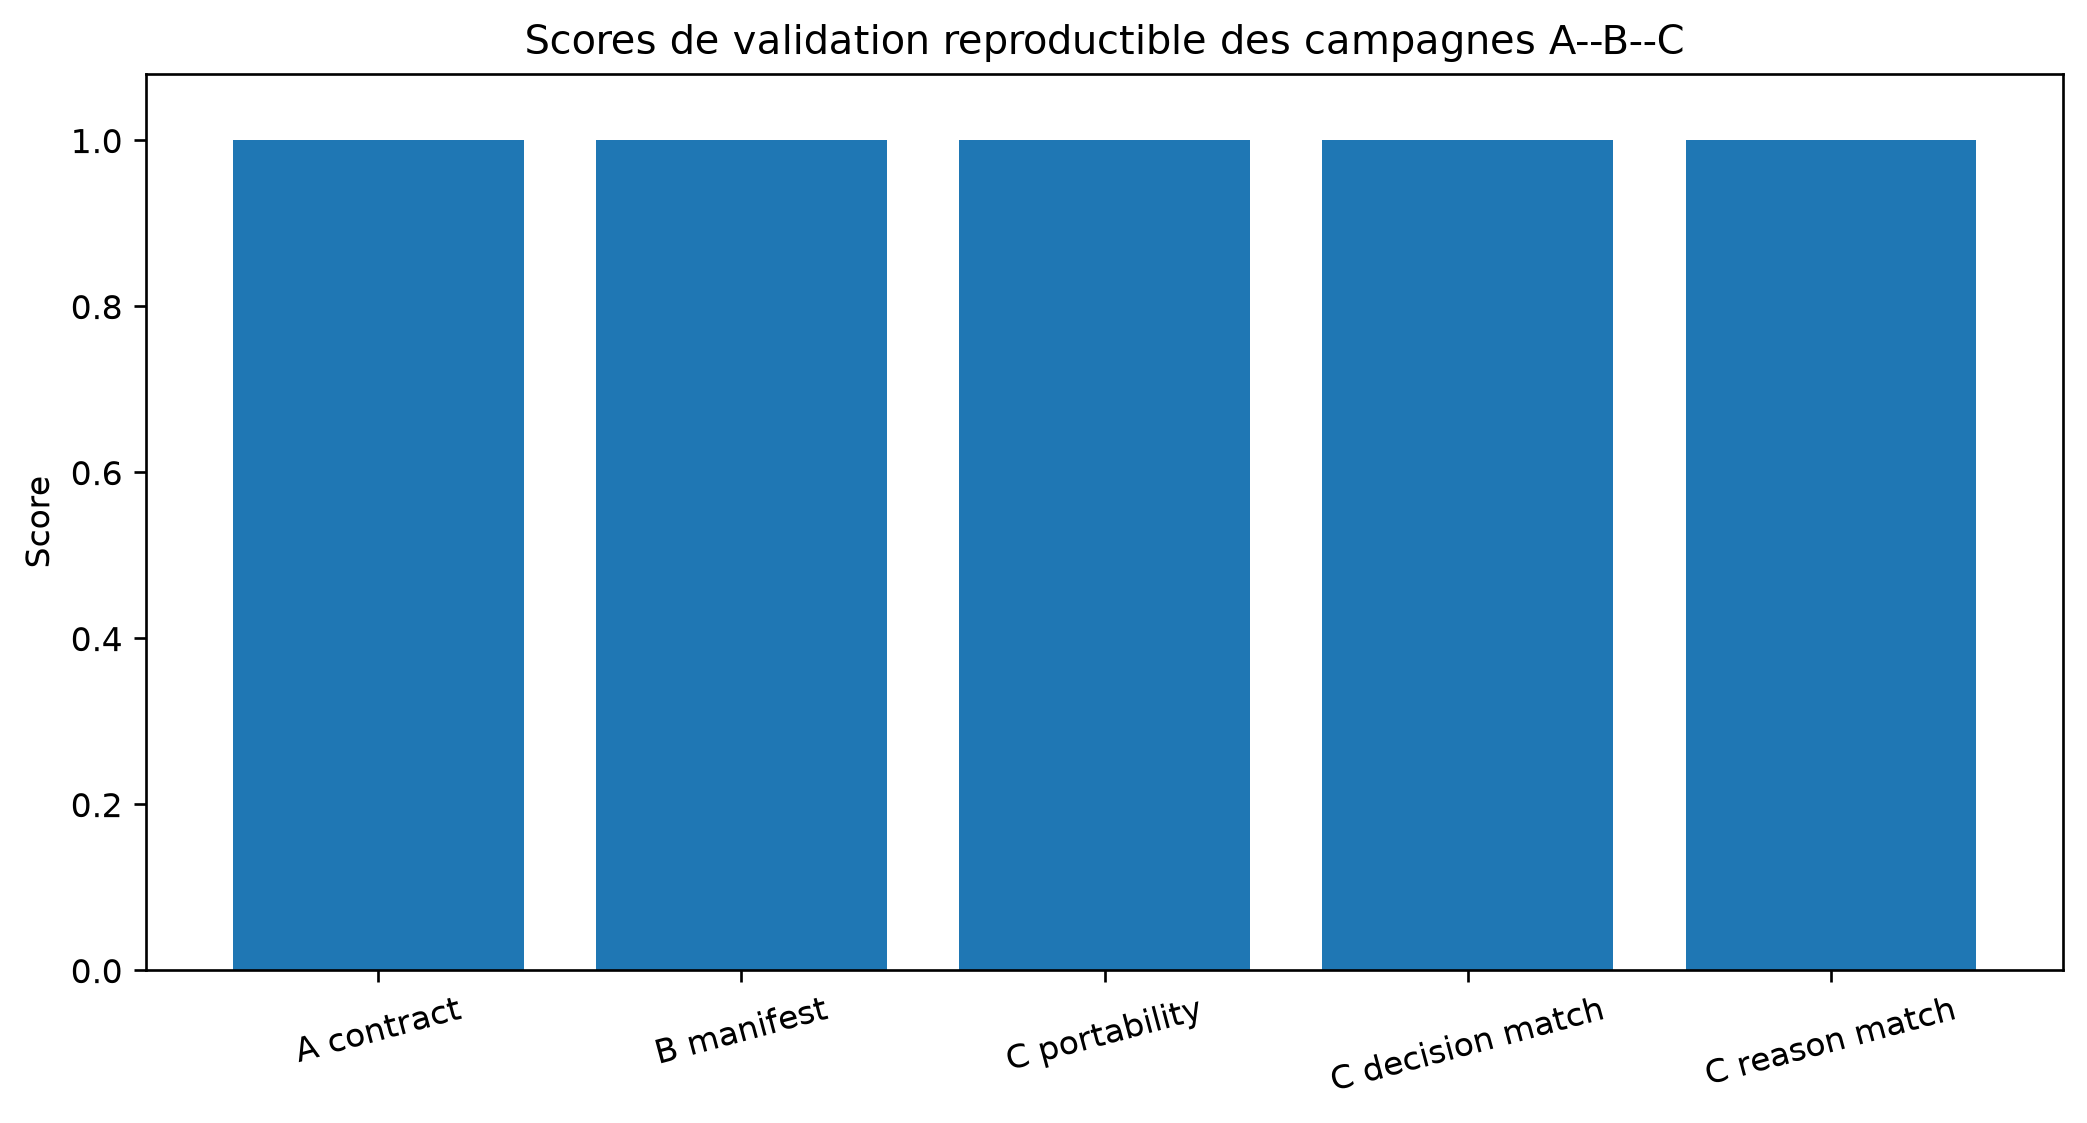
\includegraphics[width=\linewidth]{figures/human_validation_scores.png}
\caption{Validation humaine externe : comparaison entre décisions MCAD et annotations expertes.}
\label{fig:human-validation}
\end{figure}

\begin{figure}[t]
\centering
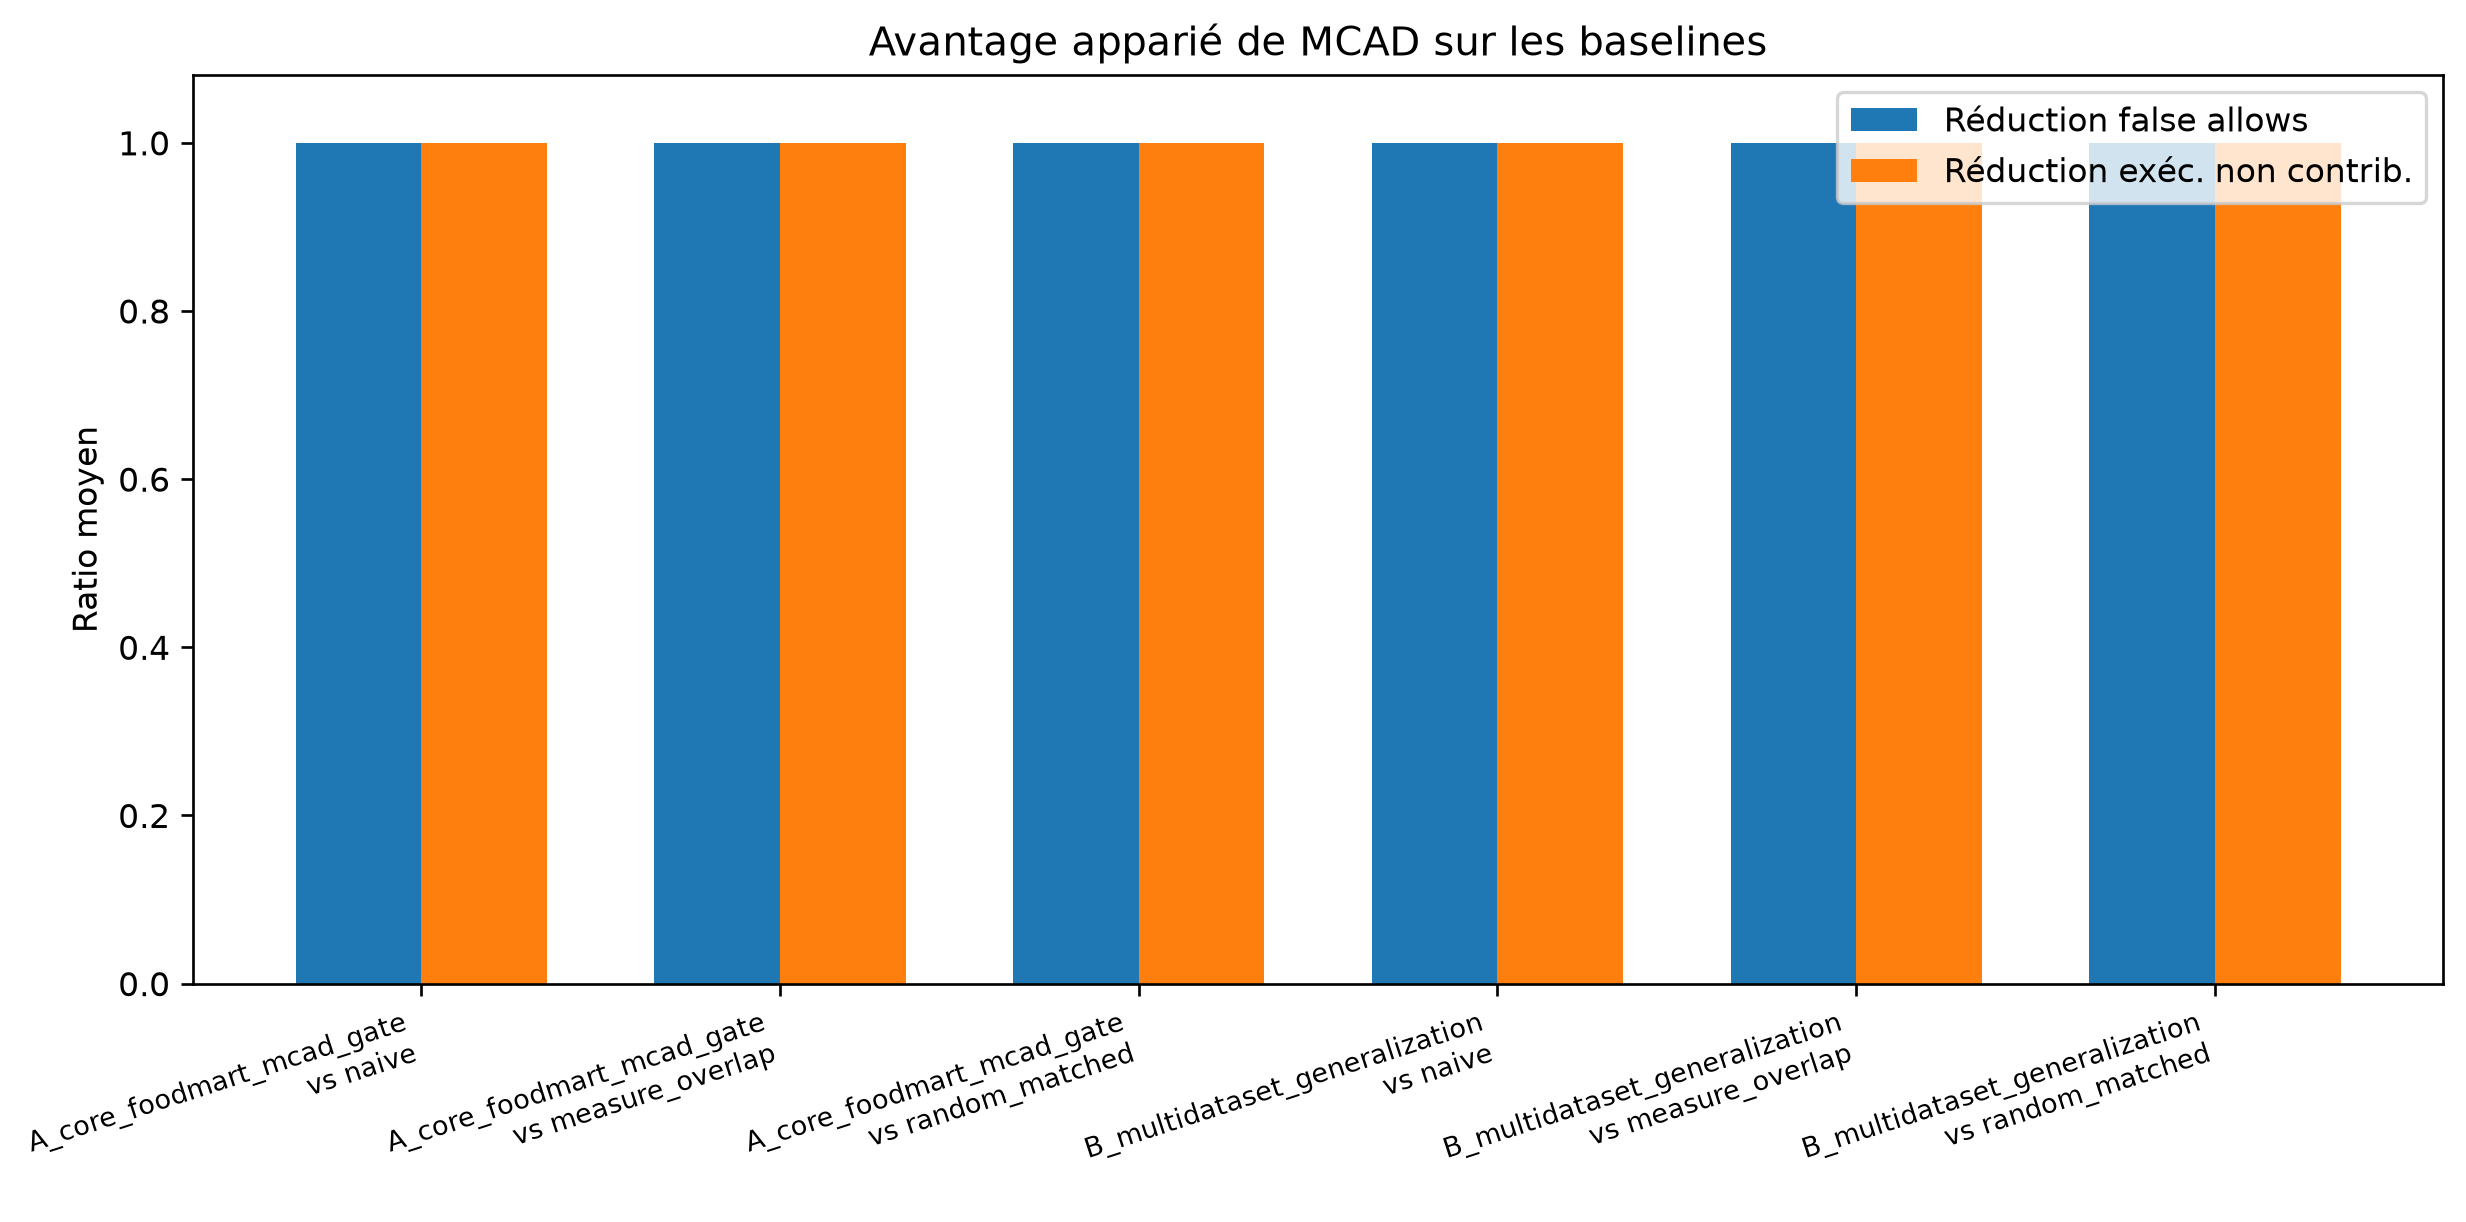
\includegraphics[width=\linewidth]{figures/mcad_advantage_false_allow.png}
\caption{Avantage apparié de MCAD sur la réduction des false allows et des exécutions non contributives.}
\label{fig:paired-advantage}
\end{figure}

\begin{figure}[t]
\centering
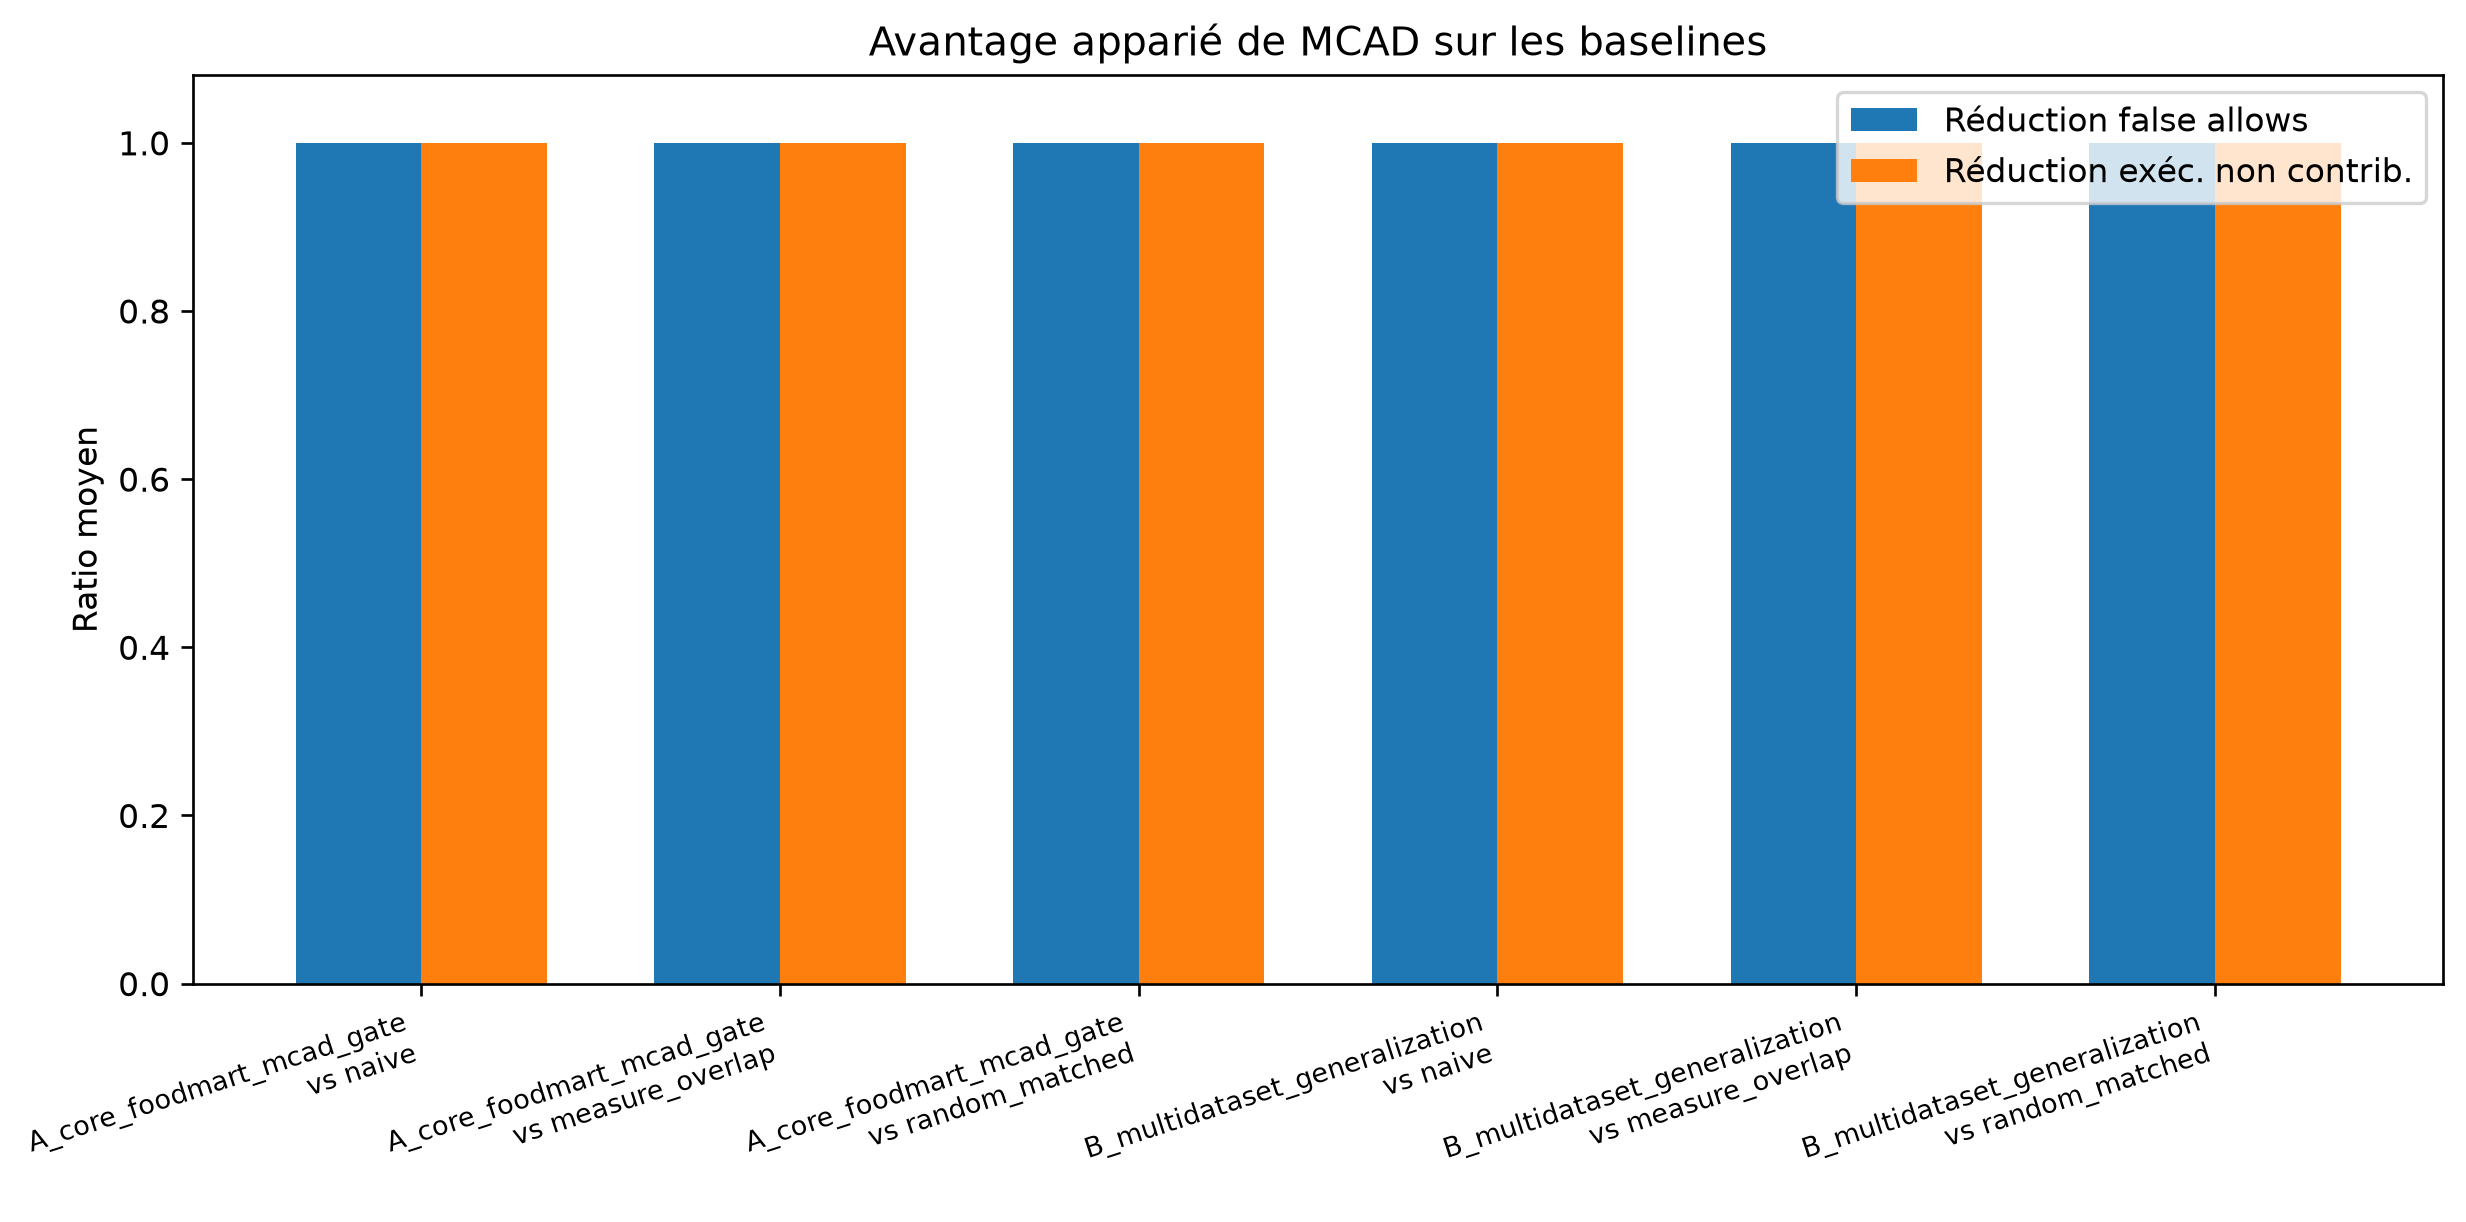
\includegraphics[width=\linewidth]{figures/fig_paired_comparative_analysis.png}
\caption{Analyse comparative appariée entre MCAD et les politiques de référence.}
\label{fig:paired-comparative-analysis}
\end{figure}

\begin{figure}[t]
\centering
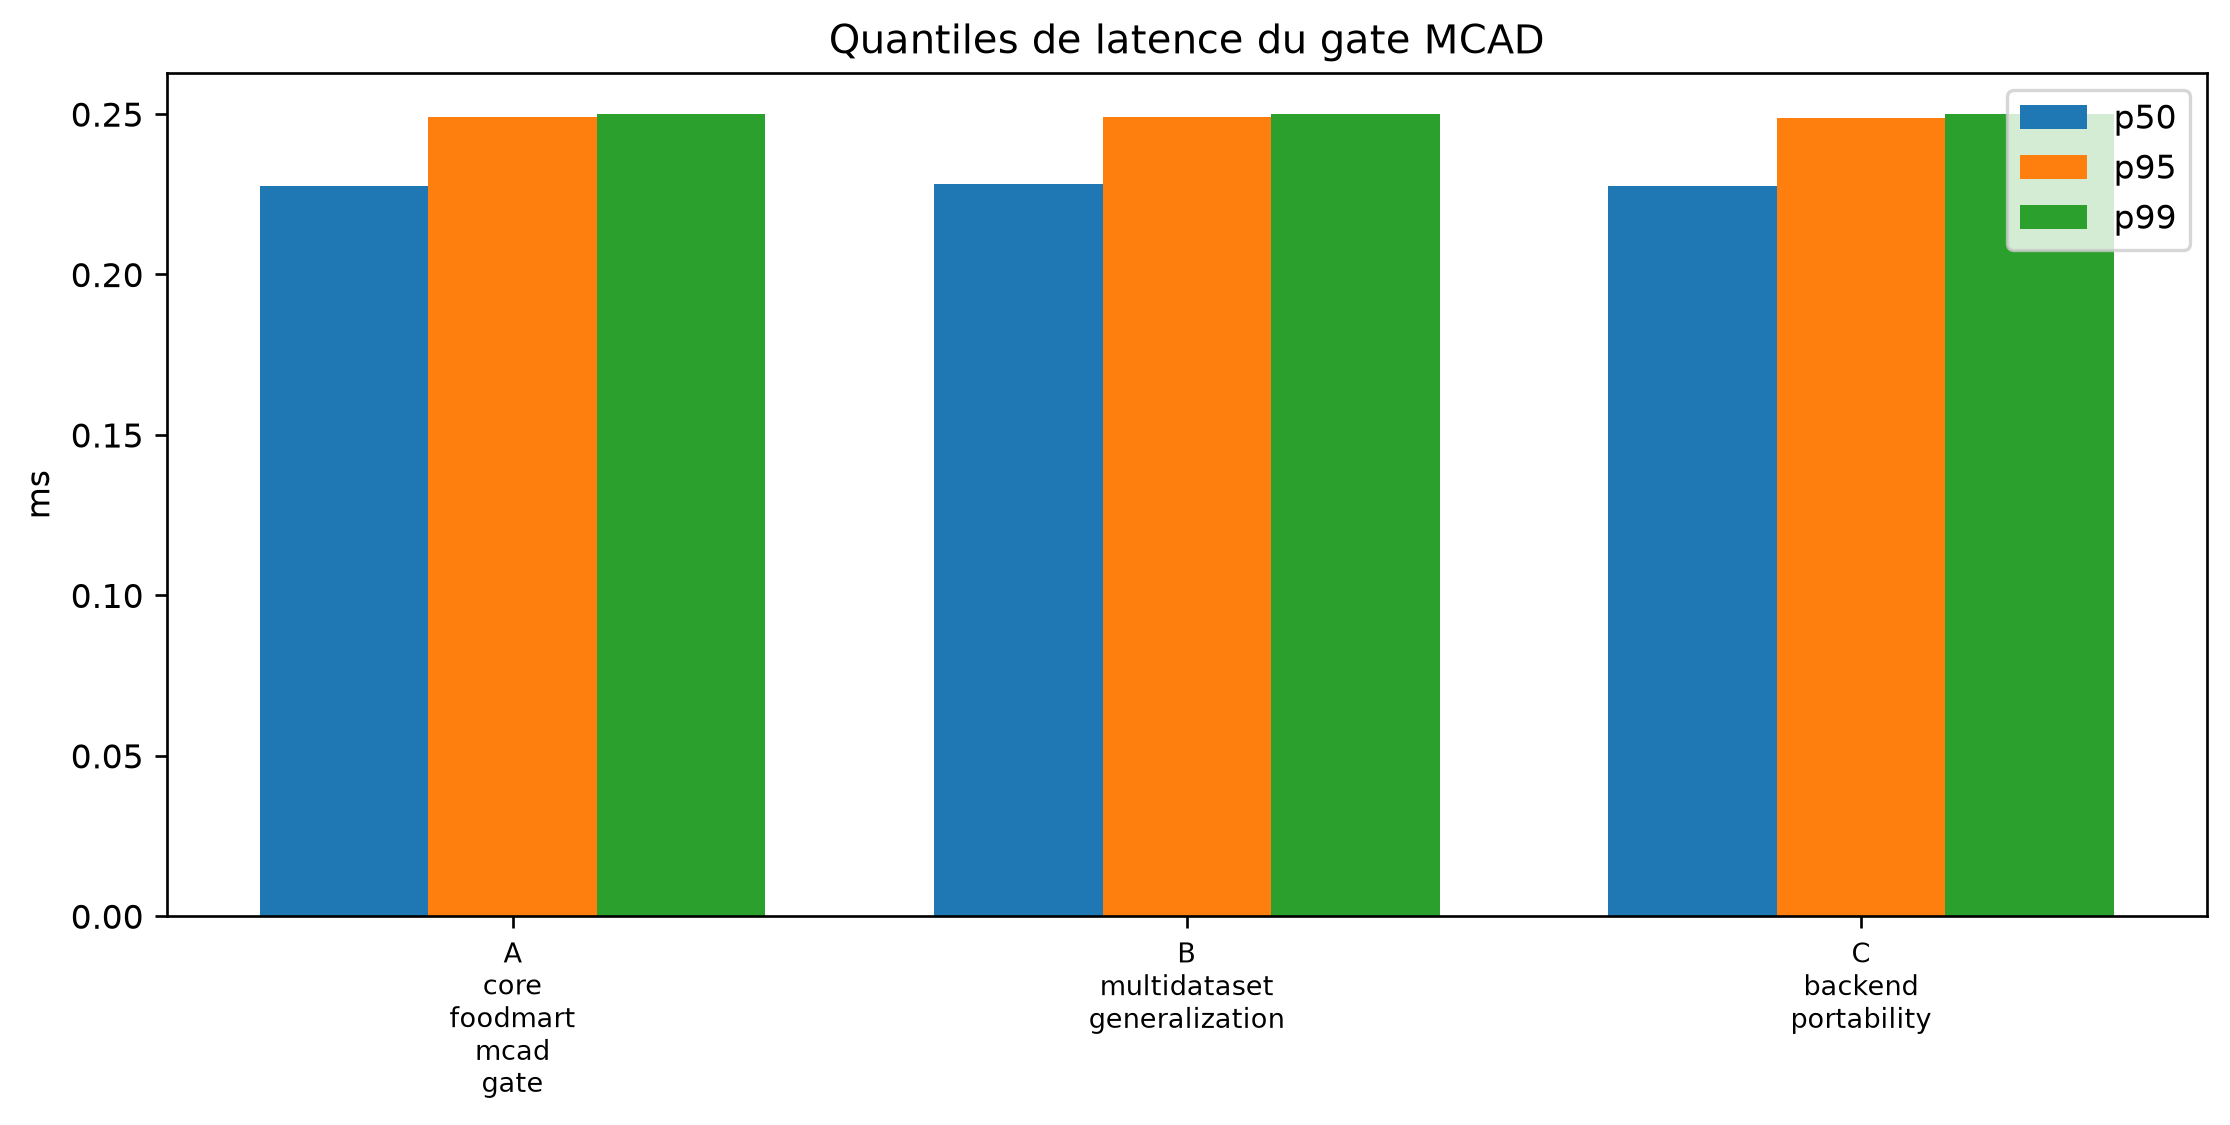
\includegraphics[width=\linewidth]{figures/fig_efficiency_explainability.png}
\caption{Synthèse efficacité--explicabilité : compromis entre filtrage stratégique, coût d'évaluation et justification des décisions.}
\label{fig:efficiency-explainability}
\end{figure}

\subsection{Campagne B : validation multi-dataset contrôlée}

La Campagne B vérifie que MCAD conserve son comportement sur plusieurs entrepôts et plusieurs backends. Elle couvre trois scénarios contrôlés : FoodMart via XMLA/Mondrian, AdventureWorksDW via SQL Server Direct et SteelWheels via SQL Server Direct. Sur 18 requêtes, MCAD produit les 18 décisions attendues. Les 7 décisions ALLOW sont exécutées physiquement, tandis que les 11 décisions BLOCK sont arrêtées avant toute exécution physique. Le CKG verrouillé de la Campagne B contient exactement 7 événements utiles, et le snapshot A reste inchangé à 2266 événements.

\begin{table}[!t]
\centering
\caption{Campagne B contrôlée : validation multi-dataset avec exécution physique.}
\scriptsize
\setlength{\tabcolsep}{4pt}
\begin{tabular}{@{}lrrrrrrr@{}}
\toprule
Scénarios & Requêtes & ALLOW & BLOCK & ALLOW physiques & BLOCK sans exéc. & Événements CKG & A verrouillé \\
\midrule
3 & 18 & 7 & 11 & 7 & 11 & 7 & 2266 \\
\bottomrule
\end{tabular}
\normalsize
\label{tab:campaign-b-controlled}
\end{table}


\subsection{Campagne C : portabilité backend AdventureWorksDW}

La Campagne C évalue une propriété différente de la Campagne B : la portabilité backend. Le même objectif AdventureWorksDW et la même séquence analytique sont exécutés dans deux sous-runs isolés, l'un via SQL Server Direct et l'autre via XMLA/eMondrian. Chaque sous-run démarre avec un CKG vide afin d'éviter qu'un backend ne bénéficie des événements créés par l'autre. Les deux chemins produisent la même séquence de décisions, les mêmes raisons de décision, la même politique d'exécution physique et deux événements CKG utiles chacun.

\begin{table*}[!t]
\centering
\caption{Campagne C : portabilité backend AdventureWorksDW SQL Direct vs XMLA/eMondrian.}
\scriptsize
\setlength{\tabcolsep}{4pt}
\begin{tabular}{@{}lrrrrrrrr@{}}
\toprule
Sous-runs & Requêtes & ALLOW & BLOCK & ALLOW physiques & BLOCK sans exéc. & Décisions identiques & Raisons identiques & CKG isolé \\
\midrule
2 & 12 & 4 & 8 & 4 & 8 & True & True & True \\
\bottomrule
\end{tabular}
\normalsize
\label{tab:campaign-c-portability}
\end{table*}


\begin{figure}[t]
\centering
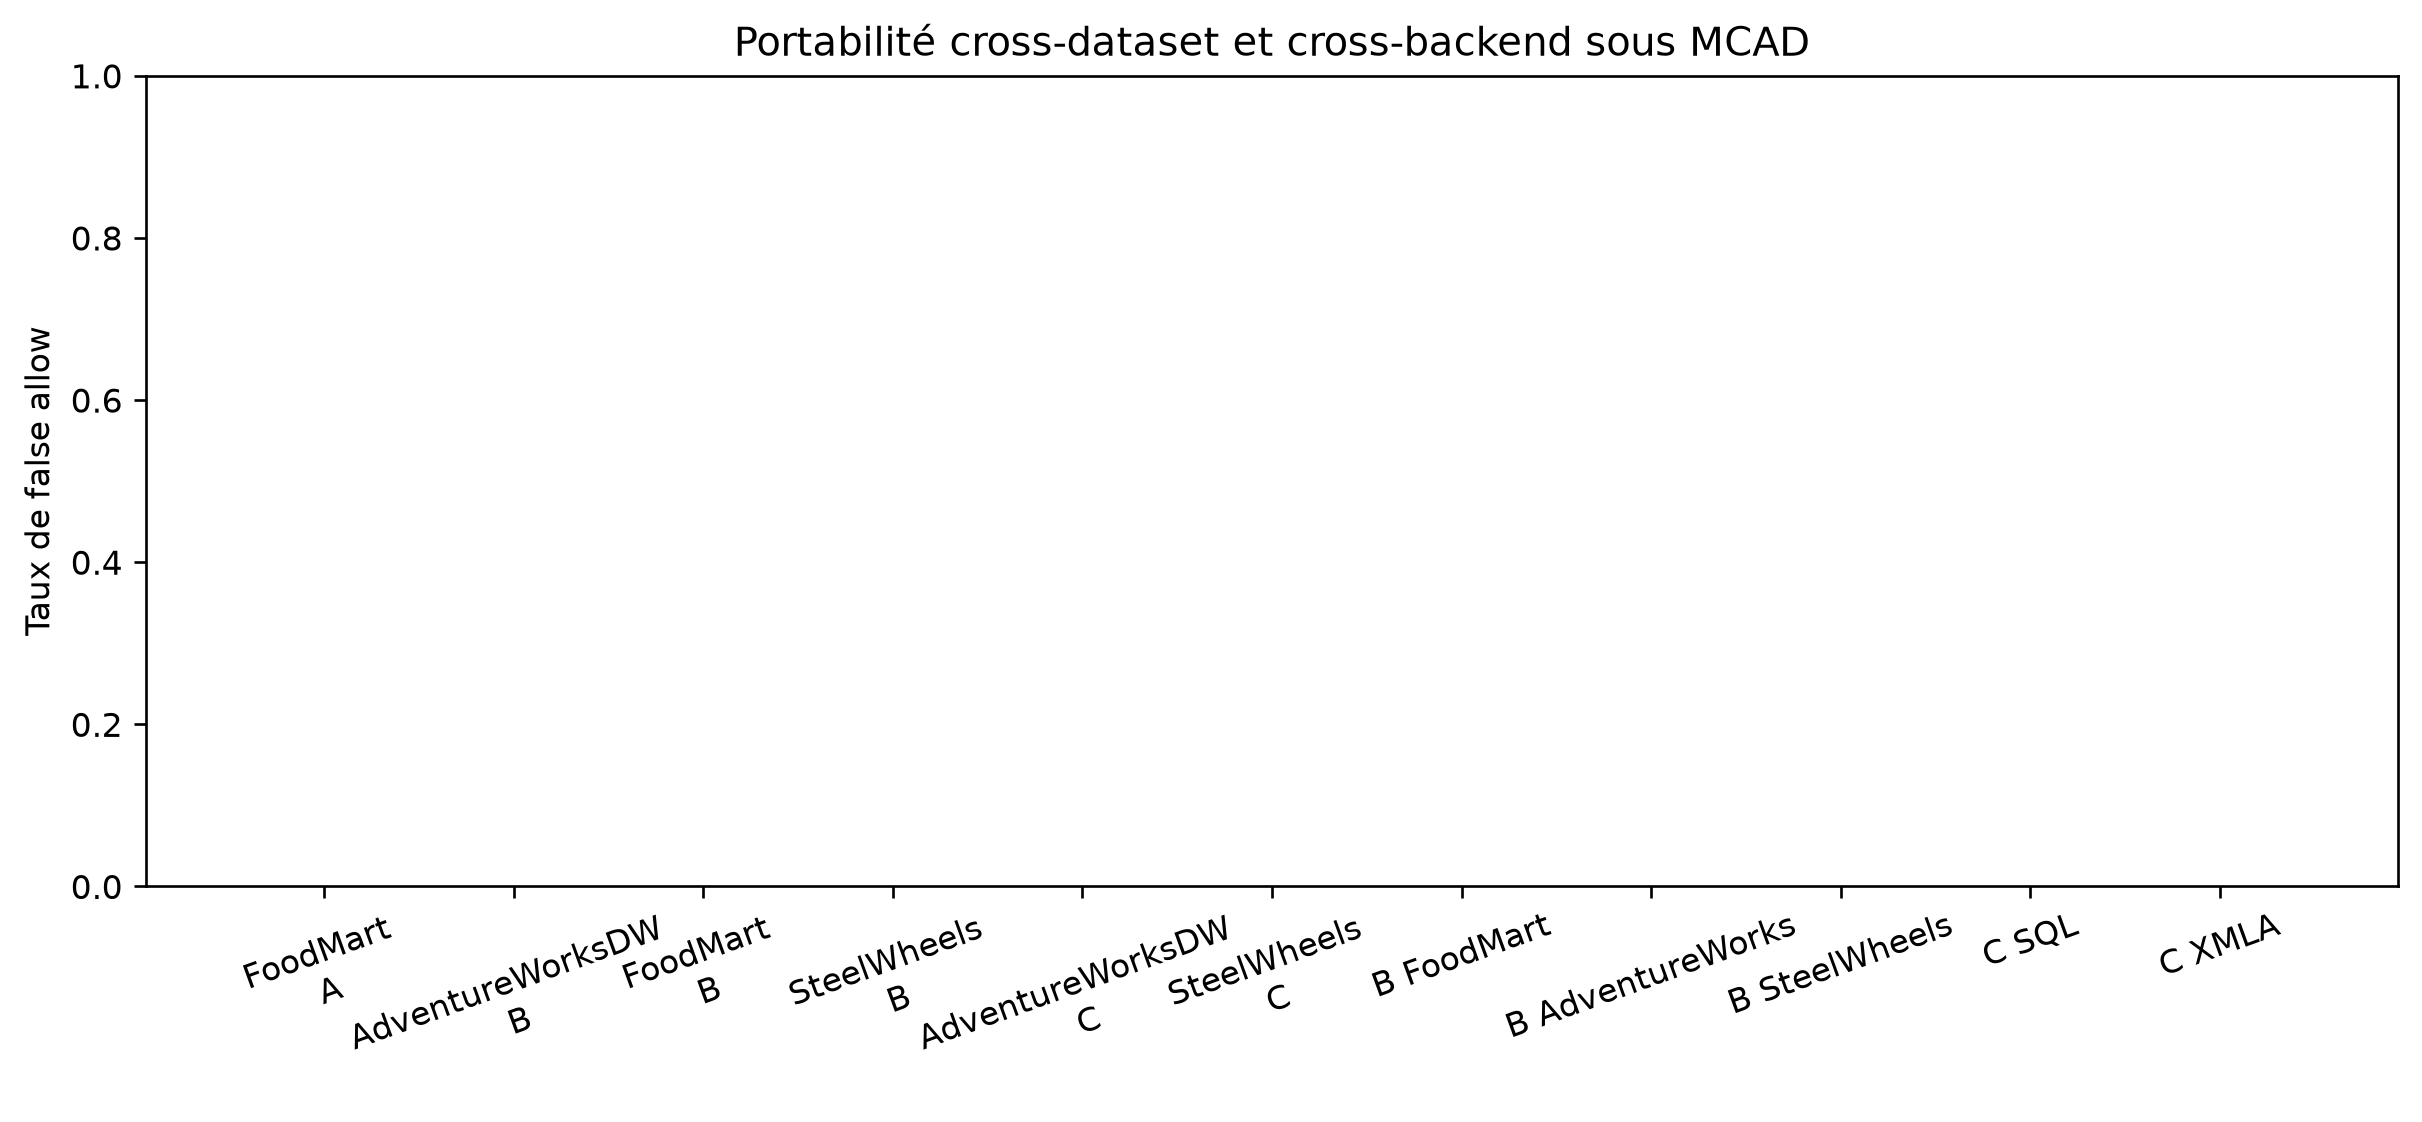
\includegraphics[width=\linewidth]{figures/fig_backend_portability.png}
\caption{Campagne C : portabilité backend AdventureWorksDW entre SQL Server Direct et XMLA/eMondrian.}
\label{fig:backend-portability}
\end{figure}

\subsection{Synthèse transversale}

Les trois campagnes ne mesurent pas la même propriété. La Campagne A établit la profondeur et la stabilité du raisonnement CKG-first sur un grand nombre de sessions. La Campagne B établit que MCAD peut être appliqué de manière contrôlée à plusieurs datasets et backends tout en préservant la séparation entre requêtes contributives et non contributives. La Campagne C établit que, pour un même objectif et une même séquence analytique, le comportement décisionnel est conservé lorsque le backend physique change.

La portée de ces résultats reste celle d'un prototype de recherche. Les expériences ne démontrent pas une supériorité universelle sur tout moteur OLAP ou toute politique analytique possible. Elles établissent cependant que la chaîne formelle proposée est exécutable, reproductible, auditable, multi-dataset et portable sur les scénarios étudiés.

% MCAD-FINAL-EXPERIMENTAL-SECTION-BEGIN
\section{Évaluation expérimentale}
\label{sec:evaluation-experimentale}

\subsection{Protocole et classes de preuve}

L'évaluation distingue strictement trois classes de preuves.
Premièrement, la trace instrumentée end-to-end canonique Q1--Q6 et
les campagnes A, B et C établissent le comportement opérationnel du
prototype et, lorsque cela est explicitement observé, le contrat
d'exécution physique. Deuxièmement, les campagnes contrôlées de
sensibilité évaluent des facteurs déclarés sur des charges communes
et selon des protocoles préenregistrés. Troisièmement, les analyses de
précision portent sur la latence de décision sémantique et ne doivent
pas être interprétées comme des mesures de latence du backend.

Aucune métrique fondée sur des annotations humaines ou expertes
(precision, recall, F1 ou $\kappa$) n'est rapportée ici, faute de
provenance canonique d'annotation permettant de soutenir ce type
d'inférence. Les requêtes Q1--Q6 constituent une seule trace
séquentielle de six étapes et ne sont donc pas traitées comme six
observations indépendantes.

\subsection{Trace canonique Q1--Q6}

La trace Q1--Q6 est exécutée sur AdventureWorksDW via l'adaptateur
SQL Server Direct. Les trois premières requêtes apportent
successivement les exigences SalesAmount, TotalProductCost et
GrossMargin. La progression cumulative de l'objectif vaut donc
$1/3$, $2/3$ puis $1$. Ces trois requêtes sont autorisées et atteignent
l'exécution physique.

Les trois étapes suivantes illustrent le fait que la satisfaisabilité
formelle ne suffit pas à autoriser une requête. Q4 est satisfaisable
mais hors du périmètre de l'objectif et est bloquée avant backend. Q5
est bloquée pour incompatibilité de granularité. Q6 est satisfaisable
et réalise intrinsèquement une exigence déjà présente, mais sa
contribution marginale est nulle; elle est donc bloquée comme
redondante. Au total, la trace contient trois ALLOW et trois BLOCK,
avec trois exécutions physiques et trois arrêts avant backend.

\subsection{Campagnes opérationnelles A, B et C}

La Campagne A constitue l'évaluation de profondeur sur FoodMart. Le
bloc consolidé comprend 1000 sessions et 7960 décisions: 2266 ALLOW
et 5694 BLOCK. Toutes les décisions ALLOW ont donné lieu à une
exécution physique, alors que tous les BLOCK ont été stoppés avant
backend. Les 2266 ALLOW ont également produit 2266 mises à jour CKG
utiles. Aucune violation du contrat d'exécution physique n'a été
observée dans ce périmètre.

La Campagne B étend ce contrat à trois scénarios contrôlés couvrant
FoodMart via XMLA/Mondrian, AdventureWorks via SQL Direct et
SteelWheels via SQL Direct. Les 18 requêtes donnent 7 ALLOW et
11 BLOCK, soit 7 exécutions physiques et 11 arrêts avant backend.
Cette campagne documente donc la portabilité observée du contrat
d'exécution physique sur les entrepôts et adaptateurs testés, sans
revendiquer une invariance universelle.

La Campagne C compare, pour AdventureWorks, les mêmes six requêtes
logiques sous SQL Direct et XMLA/eMondrian. Il s'agit de douze
évaluations mais de six requêtes logiques appariées. Les deux
conditions conservent les mêmes identifiants, le même ordre, les
mêmes décisions, les mêmes raisons et la même politique d'exécution
physique. Cette observation soutient la préservation du contrat de
décision sur ce scénario contrôlé; elle ne constitue ni une preuve
d'invariance globale entre backends ni une comparaison de leurs
performances.

\begin{table*}[t]
\centering
\caption{Synthèse des preuves expérimentales canoniques retenues pour l'article.}
\label{tab:experimental-evidence-final}
\small
\begin{tabular}{p{0.18\textwidth}p{0.18\textwidth}p{0.19\textwidth}p{0.35\textwidth}}
\hline
Bloc & Volume & Exécution physique & Résultat principal \\
\hline
Trace Q1--Q6
& 6 requêtes, une trace instrumentée
& 3 ALLOW exécutées, 3 BLOCK stoppées avant backend
& Progression cumulative de l'objectif de $1/3$ à $1$; Q4 hors périmètre, Q5 granularité incompatible, Q6 redondante. \\

Campagne A
& 1000 sessions, 7960 décisions
& 2266 exécutions physiques; 5694 BLOCK avant backend
& 2266 ALLOW, 5694 BLOCK, zéro violation du contrat d'exécution physique et 2266 mises à jour CKG utiles. \\

Campagne B
& 3 scénarios, 18 requêtes
& 7 exécutions physiques; 11 arrêts avant backend
& Validation du contrat d'exécution physique sur FoodMart/XMLA, AdventureWorks/SQL Direct et SteelWheels/SQL Direct dans le périmètre testé. \\

Campagne C
& 6 requêtes logiques appariées, 12 évaluations
& 4 exécutions physiques; 8 BLOCK
& Même ordre, mêmes décisions, mêmes raisons et même politique physique entre SQL Direct et XMLA/eMondrian sur le scénario AdventureWorks contrôlé. \\
\hline
\end{tabular}
\end{table*}

% R3E14-D17-XMLA-CLAIM-INTEGRATION-BEGIN
\subsection{Confirmation secondaire end-to-end sur XMLA/eMondrian}
\label{subsec:r3e14-xmla-resource-confirmation}

Un bloc confirmatoire secondaire complète les campagnes opérationnelles précédentes sur le
chemin AdventureWorks via XMLA/eMondrian. L'analyse préenregistrée porte sur 300 sessions
sémantiques et 900 \emph{arm-runs}; l'intégrité de mesure satisfait les 11 exigences gelées
du protocole. La comparaison primaire est \texttt{SAFE\_PRUNING} $-$
\texttt{PERMISSIVE\_GATED}. Chaque métrique repose sur 300 paires, avec correction de Holm
sur une famille de huit métriques et un niveau familial $\alpha=0.05$.

Les huit décisions primaires sont confirmées au niveau métrique. Le Tableau~\ref{tab:r3e14-xmla-primary}
reporte les valeurs déjà interprétées puis gelées avant intégration dans l'article; aucun effet,
aucune valeur de $p$ et aucun intervalle de confiance n'est recalculé ici. Le décompte 8/8
décrit les décisions métrique-spécifiques préenregistrées et ne constitue pas une nouvelle
revendication globale de bénéfice système.

\begin{table*}[t]
\centering
\caption{Confirmation métrique-spécifique sur XMLA/eMondrian:
\texttt{SAFE\_PRUNING} $-$ \texttt{PERMISSIVE\_GATED}. Les différences et variations
négatives indiquent une moyenne plus faible pour \texttt{SAFE\_PRUNING}; $p_{\mathrm{Holm}}$
est la valeur unilatérale ajustée dans la famille préenregistrée de huit métriques.}
\label{tab:r3e14-xmla-primary}
\scriptsize
\setlength{\tabcolsep}{2.4pt}
\begin{tabular}{p{0.245\textwidth}rrrrp{0.205\textwidth}r}
\toprule
Métrique & Moy. safe & Moy. permissive & $\Delta$ & Var. (\%) & IC95\% de $\Delta$ & $p_{\mathrm{Holm}}$ \\
\midrule
Exécutions backend complètes
& 5.4 & 21.6 & -16.2 & -75.0000 & $[-16.3066667,-16.0933333]$ & $7.99992{\times}10^{-5}$ \\
Requêtes backend, probes incluses
& 11.4966667 & 27.6966667 & -16.2 & -58.4908 & $[-16.3066667,-16.09]$ & $7.99992{\times}10^{-5}$ \\
Temps client (ms)
& 2991.13954 & 5484.80663 & -2493.66709 & -45.4650 & $[-2519.14638,-2469.57544]$ & $7.99992{\times}10^{-5}$ \\
CPU SQL Server ($\mu$s)
& 1054876.4 & 3112025.16 & -2057148.76 & -66.1032 & $[-2073075.16,-2041404.65]$ & $7.99992{\times}10^{-5}$ \\
I/O lecture SQL Server (octets)
& 179200 & 416358.4 & -237158.4 & -56.9602 & $[-276957.867,-193754.112]$ & $7.99992{\times}10^{-5}$ \\
I/O écriture SQL Server (octets)
& 693186.56 & 1223191.89 & -530005.333 & -43.3297 & $[-841742.037,-23389.0133]$ & $7.99992{\times}10^{-5}$ \\
Taille de réponse (octets)
& 225339.547 & 810012.513 & -584672.967 & -72.1807 & $[-588492.829,-580817.672]$ & $7.99992{\times}10^{-5}$ \\
Temps jusqu'à complétion de l'objectif (ms)
& 1577.87608 & 2098.16438 & -520.288297 & -24.7973 & $[-563.934414,-477.241028]$ & $7.99992{\times}10^{-5}$ \\
\bottomrule
\end{tabular}
\end{table*}

Le contraste secondaire \texttt{SAFE\_PRUNING} $-$
\texttt{UNGATED\_EXECUTE\_ADMISSIBLE} reste strictement descriptif et ne reçoit ni
valeur de $p$ confirmatoire ni revendication confirmatoire. Dans les valeurs gelées, le temps
client présente une différence moyenne de $-188.97934$~ms ($-5.94252\%$,
IC95\% $[-211.41263,-165.738574]$), l'I/O d'écriture SQL Server une différence moyenne
de $-188474.027$ octets avec un IC95\% incluant zéro
($[-420224.043,264453.248]$), tandis que le temps jusqu'à complétion de l'objectif est
plus élevé de $384.504904$~ms sous \texttt{SAFE\_PRUNING} ($+32.2201\%$,
IC95\% $[362.649556,406.244273]$). Ces éléments sont rapportés uniquement comme
diagnostic de \emph{break-even}.

Les diagnostics de ressources propres à eMondrian restent eux aussi descriptifs: aucun
$p$ confirmatoire ni revendication confirmatoire de réduction de ressources n'est attribué.
En particulier, les intervalles de lecture I/O eMondrian incluent zéro pour les deux
comparateurs, et l'intervalle d'écriture I/O inclut zéro face à
\texttt{PERMISSIVE\_GATED}. Aucune équivalence de backend, aucune homogénéité d'effet,
aucun test de différence d'effet entre backends et aucune synthèse cross-backend ne sont
déduits de ce bloc.
% R3E14-D17-XMLA-CLAIM-INTEGRATION-END

\begin{table*}[t]
\centering
\caption{Bilan terminal des facteurs de sensibilité contrôlée.}
\label{tab:sensitivity-final}
\small
\begin{tabular}{p{0.21\textwidth}p{0.14\textwidth}p{0.55\textwidth}}
\hline
Facteur & Stade terminal retenu & Statut de publication \\
\hline
Nombre de contraintes
& Stage 20
& Campagne canonique Stage-20 gelée; les conclusions sont bornées au protocole et au freeze associés. \\

Nombre de noeuds virtuels
& Stage 10
& Cibles de précision préenregistrées atteintes au Stage-10; aucune extension Stage-20 requise. \\

Densité d'appartenance
& Stage 10
& Décision de précision Stage-10 PASS, selon l'artefact canonique sélectionné dans le source-map final. \\

Nombre d'objectifs
& Stage 30
& Limite terminale de précision: 17/192 cellules hors cibles préenregistrées après 30 clusters et 576000 mesures; aucun rerun, aucun bootstrap supplémentaire et aucun Stage-40. \\
\hline
\end{tabular}
\end{table*}


\subsection{Sensibilité et précision de la décision sémantique}

Les facteurs contrôlés retenus pour la publication sont le nombre de
contraintes, le nombre de noeuds virtuels, la densité d'appartenance
et le nombre d'objectifs. Leur source scientifique primaire est
figée par le source-map de publication associé au présent état du
dépôt.

Pour le nombre de noeuds virtuels, les cibles de précision
préenregistrées sont atteintes au Stage-10 et aucune extension
Stage-20 n'est requise. Pour la densité d'appartenance, la décision
canonique de précision au Stage-10 est PASS. Le nombre de contraintes
est rapporté depuis la campagne canonique Stage-20 gelée.

Le nombre d'objectifs requiert l'extension préenregistrée jusqu'au
Stage-30, stade maximal du protocole. L'analyse terminale porte sur
30 clusters structurels, 576000 mesures et 192 cellules
niveau--étape. Dix-sept cellules ne satisfont pas simultanément les
cibles de précision préenregistrées. Le statut terminal est donc
\texttt{stage30\_precision\_targets\_not\_met} et
\texttt{stage30\_sufficient=false}. Ce résultat n'est pas un échec
d'exécution: l'analyse canonique s'est terminée correctement et
constitue la limite de précision terminale prévue par le protocole.
Aucune réplication supplémentaire, aucun nouveau bootstrap et aucun
Stage-40 ne sont autorisés.

\subsection{Portée des conclusions}

Les résultats soutiennent, dans les scénarios étudiés, la distinction
entre satisfaisabilité, contribution à l'objectif et décision
d'autorisation, ainsi que l'application cohérente du gate physique:
un BLOCK est arrêté avant exécution backend alors qu'un ALLOW peut
atteindre l'adaptateur d'exécution. Les résultats de sensibilité
documentent la stabilité ou les limites de précision observées pour
les facteurs contrôlés.

Ces conclusions restent bornées au prototype, aux jeux de données,
aux scénarios, aux facteurs et aux protocoles expérimentaux
considérés. Elles ne démontrent ni supériorité universelle, ni
invariance générale vis-à-vis des backends, ni robustesse
industrielle hors du périmètre évalué.

% MCAD-FINAL-EXPERIMENTAL-SECTION-END


\section{Discussion, limites et perspectives}
\label{sec:disc}

MCAD introduit une nouvelle manière d'aborder l'analyse décisionnelle : au lieu de traiter les requêtes comme des actions isolées, il les situe à l'intérieur d'un espace contextuel explicite (le CKG) et à l'intérieur d'un programme d'analyse défini par des objectifs et des contraintes. Les résultats consolidés montrent que sa force principale, à ce stade, réside dans la \emph{sélectivité stratégique} : sur les charges évaluées, MCAD élimine les exécutions non contributives et les \emph{false allows} sans dégrader la couverture finale atteinte par des politiques plus permissives.

Cette propriété rend le modèle particulièrement intéressant pour trois usages complémentaires : (i) \textbf{gouverner les usages analytiques}, en objectivant la part des requêtes réellement utiles pour un objectif donné ; (ii) \textbf{compléter la personnalisation}, en fournissant aux moteurs de recommandation une métrique stratégique explicable qui va au-delà des seules préférences utilisateur ; et (iii) \textbf{faire le lien avec l'optimisation contextuelle}, puisque les quantités $\varphi(QP,O)$ et $\Delta\varphi_t$ peuvent être interprétées comme des récompenses explicables pour des politiques séquentielles.

\subsection{Affirmations soutenues, limites et menaces à la validité}

La version courante de l'article soutient les affirmations suivantes : (i) MCAD fournit une chaîne formelle et exécutable pour relier les requêtes analytiques à des contraintes stratégiques explicites ; (ii) le cœur mathématique complet de cette chaîne est implémenté dans le prototype de recherche courant, y compris l'extraction canonique multi-langage, le $\mathrm{SAT}$ clause par clause, $\mathrm{Real}$, $C_{\mathrm{eval}}$, les masques induits $S^*$ et les sorties de contribution cumulative ; (iii) cette chaîne peut être exercée de bout en bout sur deux entrepôts de type benchmark et sur des charges dédiées de robustesse ; (iv) sur les charges étudiées, MCAD préserve la couverture utile tout en éliminant les exécutions non contributives et les \emph{false allows}, avec des décisions qui restent explicables au moyen de prédicats échoués, d'ensembles d'exigences manquantes et de masques induits renvoyés à l'exécution ; (v) la partie utile retenue des requêtes contributives est désormais persistée avec une provenance explicite et peut être réutilisée pour accélérer des sessions ultérieures sous une politique de bootstrap contrôlée et sensible à l'évidence ; et (vi) le prototype de recherche courant expose désormais un contrat de décision stable, un journal persistant d'audit de décision et un \emph{replay} déterministe sur snapshots d'évidence retenue, ce qui rend la chaîne de raisonnement plus facile à inspecter et à régresser entre versions.

À l'inverse, l'article ne prétend pas que MCAD améliore universellement la couverture finale par rapport à toutes les baselines permissives, que le prototype courant constitue déjà un middleware BI de niveau industriel, ni que l'évaluation présente épuise toutes les menaces à la généralisation. L'objectif de cette version est d'établir un résultat fort au niveau \emph{prototype de recherche}, et non de surévaluer le niveau de maturité de l'implémentation.

\paragraph*{Menaces à la validité.}

\textbf{Validité de construit.} La mesure de contribution proposée est définie par la chaîne $QP \rightarrow \mathrm{SAT} \rightarrow \mathrm{Real} \rightarrow C_{\mathrm{eval}} \rightarrow \varphi$. Une première menace est donc de savoir si cette opérationnalisation capte bien l'intuition d'utilité analytique. Nous réduisons ce risque en modélisant explicitement les objectifs comme des ensembles de contraintes et en définissant la calculabilité à partir de supports suffisants, plutôt qu'au moyen d'un simple recouvrement non vide.

\textbf{Validité interne.} Le prototype dépend d'un parseur de requêtes et de règles de matching vis-à-vis du CKG. Des erreurs dans l'extraction MDX $\rightarrow QP$, dans la normalisation temporelle ou dans la compatibilité de grain peuvent biaiser l'évaluation. Nous atténuons ce risque au moyen d'une représentation canonique de $QP$, de tests dédiés de non-régression et de scénarios couvrant spécifiquement les contraintes de croissance multi-périodes.

\textbf{Validité externe.} Une validation sur un seul entrepôt fournirait une preuve faible de généralité. Nous avons donc étendu l'évaluation au-delà de FoodMart vers un second dataset de type AdventureWorks. Malgré cela, la validité externe reste partielle : les deux schémas appartiennent à la famille des entrepôts décisionnels en étoile et les scénarios demeurent semi-synthétiques.

\textbf{Validité de conclusion.} Les résultats de benchmark peuvent dépendre du design des scénarios, des graines aléatoires ou de la difficulté relative des requêtes candidates. C'est pourquoi nous rapportons non seulement la couverture finale, mais aussi $\mathrm{AUC}(\varphi)$, les taux de \emph{false allow} / \emph{false block}, les taux d'exécutions non contributives, les latences et des comparaisons à plusieurs baselines et ablations.

\subsection{Perspectives}

Les limitations actuelles résident principalement dans l'effort initial de modélisation (construction du CKG, définition des contraintes et des nœuds virtuels), dans la dépendance à la qualité des métadonnées, et dans l'échelle encore bornée de la présente étude par annotations expertes. Bien que trois fichiers d'annotation externes aient été intégrés et scorés avec succès, la couche de validation humaine actuelle repose encore sur un pack compact de 30 items ; des panels experts plus larges, des rounds d'adjudication explicites et une couverture métier plus étendue renforceraient encore la validité externe de cette composante. Les nouveaux résultats de scalabilité indiquent que la couche de décision sémantique reste stable lorsque le CKG croît, mais ils montrent également que les coûts de persistance et d'archivage augmentent plus sensiblement que la latence de décision en ligne ; des stratégies de stockage plus riches, une persistance asynchrone et une gestion plus avancée du cycle de vie du CKG demeurent donc des directions d'ingénierie importantes. L'agrégation de plusieurs objectifs et la gestion de conflits entre contraintes restent aussi des axes de recherche majeurs.

Les travaux futurs incluent : (i) l'automatisation partielle de la construction du CKG et des nœuds virtuels à partir des schémas, journaux de requêtes et documentations ; (ii) l'intégration de politiques de recommandation et d'optimisation guidées par la contribution marginale ; (iii) l'extension aux contextes multi-objectifs ; (iv) le passage de la couche actuelle d'évidence retenue avec provenance vers des politiques de gouvernance de plus long terme pour la détection des conflits, la gestion des contradictions et la mémoire partagée multi-utilisateur ; et (v) l'étude de l'adoption de MCAD dans des plateformes BI industrielles.

\section{Conclusion}
\label{sec:conclusion}

Cet article a introduit le \emph{Masque Contextuel de l'Analyse Décisionnelle} (MCAD), un cadre visant à rendre explicite et mesurable le lien entre les requêtes OLAP et les objectifs stratégiques de l'organisation. En modélisant le contexte de l'analyse décisionnelle sous la forme d'un graphe de connaissances contextuel, en représentant les objectifs comme des ensembles de contraintes ancrées dans ce graphe par des nœuds virtuels, en abstrahant les requêtes en plans canoniques vérifiés par un prédicat explicable de validité contextuelle, et en définissant des mesures de contribution, MCAD fournit un pont opérationnel entre analyse et pilotage.

L'étude de cas FoodMart, la généralisation à un second dataset de type AdventureWorks, les campagnes de benchmark avec baselines et ablations, le benchmark d'utilité de l'évidence, et l'évaluation reproduite par annotations expertes convergent vers un même constat : la contribution la plus forte de MCAD est de rendre l'exécution analytique \emph{sélective}, \emph{explicable} et \emph{alignée} avec un objectif stratégique formalisé. Sur les charges évaluées, MCAD préserve la couverture finale atteinte par des politiques plus permissives tout en supprimant les exécutions non contributives et les \emph{false allows}, avec un faible surcoût compatible avec un usage interactif ; de plus, la partie utile retenue des requêtes contributives est déjà suffisamment opérationnelle pour soutenir une réutilisation sensible à la provenance et une récupération plus rapide de la couverture dans des sessions ultérieures, sous des conditions de bootstrap contrôlées. Le présent article doit donc être lu comme une démonstration forte, au niveau prototype, d'un filtrage stratégique des requêtes et d'une mise à jour significative du graphe, renforcée par une comparaison experte externe sur un pack borné, et non comme l'affirmation qu'une généralisation large à tout contexte d'usage serait déjà acquise.

\appendices

\section{Preuves formelles des propriétés de la Section~\ref{sec:formal}}
\label{app:proofs}

\subsection*{Preuve de la Proposition~\ref{prop:borne}}

Par définition, $C_{\mathrm{eval}}(QP,O)\subseteq C^*(O)$, d'où
\[
0\le |C_{\mathrm{eval}}(QP,O)|\le |C^*(O)|.
\]
En divisant par $|C^*(O)|>0$, on obtient $0\le \varphi(QP,O)\le 1$, ce qui prouve que $\varphi(QP,O)\in[0,1]$.

Si $C_{\mathrm{eval}}(QP,O)=\emptyset$, alors $|C_{\mathrm{eval}}(QP,O)|=0$, et donc $\varphi(QP,O)=0$. Réciproquement, si $\varphi(QP,O)=0$, alors $|C_{\mathrm{eval}}(QP,O)|=0$, d'où $C_{\mathrm{eval}}(QP,O)=\emptyset$.

Si $C_{\mathrm{eval}}(QP,O)=C^*(O)$, alors $|C_{\mathrm{eval}}(QP,O)|=|C^*(O)|$, et donc $\varphi(QP,O)=1$. Réciproquement, si $\varphi(QP,O)=1$, alors $|C_{\mathrm{eval}}(QP,O)|=|C^*(O)|$ et, comme $C_{\mathrm{eval}}(QP,O)\subseteq C^*(O)$, on conclut que $C_{\mathrm{eval}}(QP,O)=C^*(O)$. \hfill$\square$

\subsection*{Preuve de la Proposition~\ref{prop:mono-real}}

Supposons $\mathrm{Real}(QP_a)\subseteq \mathrm{Real}(QP_b)$. Soit $c\in C_{\mathrm{eval}}(QP_a,O)$. Par définition, il existe $R\in\mathcal{R}(c)$ tel que $R\subseteq \mathrm{Real}(QP_a)$. Comme $\mathrm{Real}(QP_a)\subseteq \mathrm{Real}(QP_b)$, on a aussi $R\subseteq \mathrm{Real}(QP_b)$, et donc $c\in C_{\mathrm{eval}}(QP_b,O)$. Ainsi,
\[
C_{\mathrm{eval}}(QP_a,O)\subseteq C_{\mathrm{eval}}(QP_b,O),
\]
ce qui implique $|C_{\mathrm{eval}}(QP_a,O)|\le |C_{\mathrm{eval}}(QP_b,O)|$ et donc $\varphi(QP_a,O)\le \varphi(QP_b,O)$. \hfill$\square$

\subsection*{Preuve de la Proposition~\ref{prop:session}}

Par définition,
\[
C_{\mathrm{eval}}^{\le t}(O)=\bigcup_{i=1}^{t} C_{\mathrm{eval}}(QP_i,O).
\]
Par conséquent, pour tout $t\ge 2$,
\[
C_{\mathrm{eval}}^{\le t-1}(O)\subseteq C_{\mathrm{eval}}^{\le t}(O),
\]
ce qui implique
\[
|C_{\mathrm{eval}}^{\le t-1}(O)|\le |C_{\mathrm{eval}}^{\le t}(O)|.
\]
En divisant par $|C^*(O)|>0$, on obtient
\[
\varphi^{\le t-1}(O)\le \varphi^{\le t}(O),
\]
de sorte que la suite $(\varphi^{\le t}(O))$ est monotone non décroissante. Comme $C_{\mathrm{eval}}^{\le t}(O)\subseteq C^*(O)$ pour tout $t$, elle est également bornée dans $[0,1]$. Enfin, $\Delta\varphi_t=\varphi^{\le t}(O)-\varphi^{\le t-1}(O)\ge 0$ découle directement de cette monotonie. \hfill$\square$

\section{Formalisation détaillée de l'exemple FoodMart HF/North}
\label{app:foodmart}

Nous revenons à l'exemple de la Section~\ref{sec:case}. Le cube \textit{Sales} est défini par :
\begin{itemize}
  \item $F=\{\textit{Sales}\}$,
  \item trois dimensions $D=\{\textit{Time},\textit{Product},\textit{Store}\}$, et
  \item des mesures $M=\{\mathrm{Store\ Sales},\mathrm{Store\ Cost},\mathrm{Units\ Sold}\}$ ainsi qu'un KPI dérivé $\mathrm{Margin\%}$.
\end{itemize}

Les hiérarchies de dimensions sont :
\begin{itemize}
  \item Time : Day $\rightarrow$ Month $\rightarrow$ Year,
  \item Product : Product $\rightarrow$ Subcategory $\rightarrow$ Category,
  \item Store : Store $\rightarrow$ City $\rightarrow$ Region.
\end{itemize}

L'objectif $O_{\mathrm{HF\_NORD}}$ est défini comme en Section~\ref{sec:case}, avec $C^*(O_{\mathrm{HF\_NORD}})=\{c_1,c_2,c_3\}$. Chaque contrainte est associée à un ensemble de nœuds virtuels :
\begin{itemize}
  \item $N(c_1)$ contient des nœuds de la forme
  \[
  nv_{1,m}=(\textit{Sales},g_m,\mathrm{Margin\%},\mathrm{avg},\%,S_{\mathrm{HF,North}},w_{1998}),
  \]
  où $g_m$ est un grain \{Month, Category=Health Food, Region=North\}, où $S_{\mathrm{HF,North}}$ restreint la catégorie à Health Food et la région à North, et où $w_{1998}$ est la fenêtre temporelle correspondant à l'année 1998.
  \item $N(c_2)$ contient des nœuds de la forme
  \[
  nv_{2,r}=(\textit{Sales},g_r,\mathrm{StockoutRate},\mathrm{ratio},\%,S_{\mathrm{HF,North}},w_{1998}),
  \]
  où $g_r$ est un grain \{Store, Category=Health Food, Region=North\} et où $\mathrm{StockoutRate}$ est un KPI dérivé de \textit{Units Sold} et d'informations de stock.
  \item $N(c_3)$ contient des nœuds de la forme
  \[
  nv_{3,m}=(\textit{Sales},g_m,\mathrm{Sales},\mathrm{sum},\text{USD},S_{\mathrm{HF,North}},w_{1997\_1998}),
  \]
  où $\mathrm{Sales}=\mathrm{Store\ Sales}$ et $w_{1997\_1998}$ couvre les années 1997 et 1998.
\end{itemize}

Considérons par exemple la requête guidée $QP'_1$ :
\[
QP'_1=(\textit{Sales},g_m,\{\mathrm{Margin\%}\},\{\mathrm{avg}\},\{\%\},S_{\mathrm{HF,North}},w_{1998}).
\]
Sous des hypothèses raisonnables de compatibilité dans le CKG, on obtient
\[
\mathrm{Real}(QP'_1)\supseteq \{nv_{1,m}\mid m\in \text{mois de 1998}\},
\]
et donc $c_1\in C_{\mathrm{eval}}(QP'_1,O_{\mathrm{HF\_NORD}})$. Si aucune cellule de $N(c_2)$ ou $N(c_3)$ n'est réalisable par $QP'_1$, alors
\[
C_{\mathrm{eval}}(QP'_1,O_{\mathrm{HF\_NORD}})=\{c_1\}
\quad\text{et}\quad
\varphi(QP'_1,O_{\mathrm{HF\_NORD}})=\frac{1}{3}.
\]
De même, les requêtes $QP'_2$ et $QP'_3$ sont construites de manière à réaliser respectivement des nœuds de $N(c_2)$ et $N(c_3)$, ce qui permet à la session $(QP'_1,QP'_2,QP'_3)$ d'atteindre rapidement une couverture complète des contraintes de l'objectif.

\begin{thebibliography}{23}

\bibitem{ChaudhuriDayal97}
S.~Chaudhuri and U.~Dayal, ``An overview of data warehousing and OLAP technology,'' \emph{ACM SIGMOD Record}, vol.~26, no.~1, pp.~65--74, 1997.

\bibitem{KimballRoss2013}
R.~Kimball and M.~Ross, \emph{The Data Warehouse Toolkit: The Definitive Guide to Dimensional Modeling}, 3rd~ed. Hoboken, NJ, USA: Wiley, 2013.

\bibitem{ChenBI2012}
H.~Chen, R.~H.~L. Chiang, and V.~C. Storey, ``Business intelligence and analytics: from big data to big impact,'' \emph{MIS Quarterly}, vol.~36, no.~4, pp.~1165--1188, 2012.

\bibitem{AissiGouider2012}
S.~Aissi and M.~S. Gouider, ``Towards the next generation of data warehouse personalization system: a survey and a comparative study,'' \emph{CoRR}, abs/1208.0203, 2012.

\bibitem{GarrigosER2009}
I.~Garrig\'os, J.~Pardillo, J.~N. Maz\'on, and J.~Trujillo, ``A conceptual modeling approach for OLAP personalization,'' in \emph{Conceptual Modeling -- ER 2009}, LNCS~5829. Berlin, Germany: Springer, 2009, pp.~401--414.

\bibitem{AligonDSS2015}
J.~Aligon, E.~Gallinucci, M.~Golfarelli, P.~Marcel, and S.~Rizzi, ``A collaborative filtering approach for recommending OLAP sessions,'' \emph{Decision Support Systems}, vol.~69, pp.~20--30, 2015.

\bibitem{HoganKGSurvey2021}
A.~Hogan \emph{et al.}, ``Knowledge graphs,'' \emph{ACM Computing Surveys}, vol.~54, no.~4, art.~71, 2021.

\bibitem{DiamantiniKPISurvey2025}
C.~Diamantini, T.~Khan, D.~Potena, and E.~Storti, ``Semantic models of performance indicators: A systematic survey,'' \emph{ACM Computing Surveys}, vol.~57, no.~8, Art.~202, 2025.

\bibitem{Niedritis2011}
A.~Niedritis, L.~Niedrite, and N.~Kozmina, ``Performance measurement framework with formal indicator definitions,'' in \emph{Perspectives in Business Informatics Research (BIR 2011)}, LNBIP~90. Berlin, Germany: Springer, 2011, pp.~44--58.

\bibitem{RomeroAbello2010}
O.~Romero and A.~Abell\'o, ``Automatic validation of requirements to support multidimensional design,'' \emph{Data \& Knowledge Engineering}, vol.~69, no.~9, pp.~917--942, 2010.

\bibitem{SadanaEJOR2025}
U.~Sadana, A.~Chenreddy, E.~Delage, A.~Forel, E.~Frejinger, and T.~Vidal, ``A survey of contextual optimization methods for decision-making under uncertainty,'' \emph{European Journal of Operational Research}, vol.~320, no.~2, pp.~271--289, 2025.

\bibitem{RoyContextOLAP2022}
S.~Roy, A.~Cortesi, and S.~Sen, ``Context-aware OLAP for textual data warehouses,'' \emph{International Journal of Information Management Data Insights}, vol.~2, no.~2, art.~100129, 2022.

\bibitem{AdomaviciusTuzhilin2011}
G.~Adomavicius, B.~Mobasher, F.~Ricci, and A.~Tuzhilin, ``Context-aware recommender systems,'' \emph{AI Magazine}, vol.~32, no.~3, pp.~67--80, 2011.

\bibitem{KeeneyRaiffa1976}
R.~L. Keeney and H.~Raiffa, \emph{Decisions with Multiple Objectives: Preferences and Value Tradeoffs}. New York, NY, USA: Wiley, 1976.

\bibitem{AuerBandit2002}
P.~Auer, N.~Cesa-Bianchi, and P.~Fischer, ``Finite-time analysis of the multiarmed bandit problem,'' \emph{Machine Learning}, vol.~47, nos.~2--3, pp.~235--256, 2002.

\bibitem{ZhouBanditSurvey2015}
L.~Zhou, ``A survey on contextual multi-armed bandits,'' \emph{CoRR}, abs/1508.03326, 2015.

\bibitem{Pourshahid2014}
A.~Pourshahid, I.~Johari, G.~Richards, D.~Amyot, and O.~Akhigbe, ``A goal-oriented, business intelligence-supported decision-making methodology,'' \emph{Decision Analytics}, vol.~1, art.~9, 2014.

\bibitem{Etcheverry2014}
L.~Etcheverry, A.~Vaisman, and E.~Zim\'anyi, ``Modeling and querying data warehouses on the Semantic Web using QB4OLAP,'' in \emph{Data Warehousing and Knowledge Discovery}, LNCS~8646. Cham, Switzerland: Springer, 2014, pp.~45--56.

\bibitem{W3CDataCube2014}
W3C, ``The RDF Data Cube Vocabulary,'' W3C Recommendation, Jan.~2014.

\bibitem{W3CSHACL2017}
W3C, ``Shapes Constraint Language (SHACL),'' W3C Recommendation, Jul.~2017.

\bibitem{W3CPROVO2013}
W3C, ``PROV-O: The PROV Ontology,'' W3C Recommendation, Apr.~2013.

\bibitem{FarihaMeliou2019}
A.~Fariha and A.~Meliou, ``Example-driven query intent discovery: abductive reasoning using semantic similarity,'' \emph{Proceedings of the VLDB Endowment}, vol.~12, no.~11, pp.~1262--1275, 2019.

\bibitem{NebotBerlanga2012}
V.~Nebot and R.~Berlanga, ``Building data warehouses with semantic Web data,'' \emph{Decision Support Systems}, vol.~52, no.~4, pp.~853--868, 2012.


\bibitem{JacobGunklachMaedche2025}
K.~Jacob, J.~Gunklach, and A.~M\"adche, ``Personalization in business intelligence and analytics systems: A state-of-the-art review and conceptualization,'' in \emph{ECIS 2025 Proceedings}, 2025.

\bibitem{GunklachNadj2023}
J.~Gunklach and M.~Nadj, ``Guidance in business intelligence \& analytics systems: A review and research agenda,'' in \emph{ECIS 2023 Research Papers}, 2023.

\bibitem{ArenasExploratory2025}
M.~Arenas \emph{et al.}, ``Exploring exploratory querying,'' \emph{Proceedings of the VLDB Endowment}, vol.~18, no.~13, pp.~5731--5739, 2025.

\bibitem{SchuetzSerafiniBozzato2021}
C.~G. Schuetz, L.~Bozzato, M.~Serafini, and G.~A. Atemezing, ``Knowledge graph OLAP: A multidimensional model and query operations for contextualized knowledge graphs,'' \emph{Semantic Web}, vol.~12, no.~6, pp.~973--1009, 2021.

\bibitem{StaudingerSchuetzSchrefl2025}
S.~Staudinger, C.~G. Schuetz, and M.~Schrefl, ``Knowledge graph support for descriptive business analytics,'' \emph{DECISION}, vol.~52, no.~3, pp.~1--31, 2025.

\bibitem{KostopoulosXAIDSS2024}
G.~Kostopoulos, K.~Al-Hayani, H.~Ali, and N.~Kumar, ``Explainable artificial intelligence-based decision support systems: A recent review,'' \emph{Electronics}, vol.~13, no.~14, art.~2842, 2024.

\end{thebibliography}

\end{document}
